\documentclass[twoside]{book}

% Packages required by doxygen
\usepackage{fixltx2e}
\usepackage{calc}
\usepackage{doxygen}
\usepackage[export]{adjustbox} % also loads graphicx
\usepackage{graphicx}
\usepackage[utf8]{inputenc}
\usepackage{makeidx}
\usepackage{multicol}
\usepackage{multirow}
\PassOptionsToPackage{warn}{textcomp}
\usepackage{textcomp}
\usepackage[nointegrals]{wasysym}
\usepackage[table]{xcolor}

% Font selection
\usepackage[T1]{fontenc}
\usepackage[scaled=.90]{helvet}
\usepackage{courier}
\usepackage{amssymb}
\usepackage{sectsty}
\renewcommand{\familydefault}{\sfdefault}
\allsectionsfont{%
  \fontseries{bc}\selectfont%
  \color{darkgray}%
}
\renewcommand{\DoxyLabelFont}{%
  \fontseries{bc}\selectfont%
  \color{darkgray}%
}
\newcommand{\+}{\discretionary{\mbox{\scriptsize$\hookleftarrow$}}{}{}}

% Page & text layout
\usepackage{geometry}
\geometry{%
  a4paper,%
  top=2.5cm,%
  bottom=2.5cm,%
  left=2.5cm,%
  right=2.5cm%
}
\tolerance=750
\hfuzz=15pt
\hbadness=750
\setlength{\emergencystretch}{15pt}
\setlength{\parindent}{0cm}
\setlength{\parskip}{3ex plus 2ex minus 2ex}
\makeatletter
\renewcommand{\paragraph}{%
  \@startsection{paragraph}{4}{0ex}{-1.0ex}{1.0ex}{%
    \normalfont\normalsize\bfseries\SS@parafont%
  }%
}
\renewcommand{\subparagraph}{%
  \@startsection{subparagraph}{5}{0ex}{-1.0ex}{1.0ex}{%
    \normalfont\normalsize\bfseries\SS@subparafont%
  }%
}
\makeatother

% Headers & footers
\usepackage{fancyhdr}
\pagestyle{fancyplain}
\fancyhead[LE]{\fancyplain{}{\bfseries\thepage}}
\fancyhead[CE]{\fancyplain{}{}}
\fancyhead[RE]{\fancyplain{}{\bfseries\leftmark}}
\fancyhead[LO]{\fancyplain{}{\bfseries\rightmark}}
\fancyhead[CO]{\fancyplain{}{}}
\fancyhead[RO]{\fancyplain{}{\bfseries\thepage}}
\fancyfoot[LE]{\fancyplain{}{}}
\fancyfoot[CE]{\fancyplain{}{}}
\fancyfoot[RE]{\fancyplain{}{\bfseries\scriptsize Generated by Doxygen }}
\fancyfoot[LO]{\fancyplain{}{\bfseries\scriptsize Generated by Doxygen }}
\fancyfoot[CO]{\fancyplain{}{}}
\fancyfoot[RO]{\fancyplain{}{}}
\renewcommand{\footrulewidth}{0.4pt}
\renewcommand{\chaptermark}[1]{%
  \markboth{#1}{}%
}
\renewcommand{\sectionmark}[1]{%
  \markright{\thesection\ #1}%
}

% Indices & bibliography
\usepackage{natbib}
\usepackage[titles]{tocloft}
\setcounter{tocdepth}{3}
\setcounter{secnumdepth}{5}
\makeindex

% Hyperlinks (required, but should be loaded last)
\usepackage{ifpdf}
\ifpdf
  \usepackage[pdftex,pagebackref=true]{hyperref}
\else
  \usepackage[ps2pdf,pagebackref=true]{hyperref}
\fi
\hypersetup{%
  colorlinks=true,%
  linkcolor=blue,%
  citecolor=blue,%
  unicode%
}

% Custom commands
\newcommand{\clearemptydoublepage}{%
  \newpage{\pagestyle{empty}\cleardoublepage}%
}

\usepackage{caption}
\captionsetup{labelsep=space,justification=centering,font={bf},singlelinecheck=off,skip=4pt,position=top}

%===== C O N T E N T S =====

\begin{document}

% Titlepage & ToC
\hypersetup{pageanchor=false,
             bookmarksnumbered=true,
             pdfencoding=unicode
            }
\pagenumbering{alph}
\begin{titlepage}
\vspace*{7cm}
\begin{center}%
{\Large pse20 }\\
\vspace*{1cm}
{\large Generated by Doxygen 1.8.13}\\
\end{center}
\end{titlepage}
\clearemptydoublepage
\pagenumbering{roman}
\tableofcontents
\clearemptydoublepage
\pagenumbering{arabic}
\hypersetup{pageanchor=true}

%--- Begin generated contents ---
\chapter{Namespace Index}
\section{Namespace List}
Here is a list of all namespaces with brief descriptions\+:\begin{DoxyCompactList}
\item\contentsline{section}{\hyperlink{namespacepewpewlaz0rt4nk}{pewpewlaz0rt4nk} }{\pageref{namespacepewpewlaz0rt4nk}}{}
\item\contentsline{section}{\hyperlink{namespacetest}{test} }{\pageref{namespacetest}}{}
\item\contentsline{section}{\hyperlink{namespacetester}{tester} }{\pageref{namespacetester}}{}
\end{DoxyCompactList}

\chapter{Hierarchical Index}
\section{Class Hierarchy}
This inheritance list is sorted roughly, but not completely, alphabetically\+:\begin{DoxyCompactList}
\item Exception\begin{DoxyCompactList}
\item \contentsline{section}{Beam\+Error}{\pageref{classpewpewlaz0rt4nk_1_1_beam_error}}{}
\begin{DoxyCompactList}
\item \contentsline{section}{Beam\+Request\+Error}{\pageref{classpewpewlaz0rt4nk_1_1_beam_request_error}}{}
\item \contentsline{section}{Beam\+Response\+Error}{\pageref{classpewpewlaz0rt4nk_1_1_beam_response_error}}{}
\end{DoxyCompactList}
\end{DoxyCompactList}
\item \contentsline{section}{http\+\_\+request\+\_\+struct}{\pageref{structhttp__request__struct}}{}
\item object\begin{DoxyCompactList}
\item \contentsline{section}{Beam}{\pageref{classpewpewlaz0rt4nk_1_1_beam}}{}
\item \contentsline{section}{Laz0r\+Cannon}{\pageref{classpewpewlaz0rt4nk_1_1_laz0r_cannon}}{}
\item \contentsline{section}{Response}{\pageref{classpewpewlaz0rt4nk_1_1_response}}{}
\end{DoxyCompactList}
\item \contentsline{section}{string\+\_\+struct}{\pageref{structstring__struct}}{}
\item \contentsline{section}{String\+Hash\+List}{\pageref{struct_string_hash_list}}{}
\item \contentsline{section}{String\+Hash\+Struct}{\pageref{struct_string_hash_struct}}{}
\end{DoxyCompactList}

\chapter{Data Structure Index}
\section{Data Structures}
Here are the data structures with brief descriptions\+:\begin{DoxyCompactList}
\item\contentsline{section}{\hyperlink{classpewpewlaz0rt4nk_1_1_beam}{Beam} }{\pageref{classpewpewlaz0rt4nk_1_1_beam}}{}
\item\contentsline{section}{\hyperlink{classpewpewlaz0rt4nk_1_1_beam_error}{Beam\+Error} }{\pageref{classpewpewlaz0rt4nk_1_1_beam_error}}{}
\item\contentsline{section}{\hyperlink{classpewpewlaz0rt4nk_1_1_beam_request_error}{Beam\+Request\+Error} }{\pageref{classpewpewlaz0rt4nk_1_1_beam_request_error}}{}
\item\contentsline{section}{\hyperlink{classpewpewlaz0rt4nk_1_1_beam_response_error}{Beam\+Response\+Error} }{\pageref{classpewpewlaz0rt4nk_1_1_beam_response_error}}{}
\item\contentsline{section}{\hyperlink{structhttp__request__struct}{http\+\_\+request\+\_\+struct} }{\pageref{structhttp__request__struct}}{}
\item\contentsline{section}{\hyperlink{classpewpewlaz0rt4nk_1_1_laz0r_cannon}{Laz0r\+Cannon} }{\pageref{classpewpewlaz0rt4nk_1_1_laz0r_cannon}}{}
\item\contentsline{section}{\hyperlink{classpewpewlaz0rt4nk_1_1_response}{Response} }{\pageref{classpewpewlaz0rt4nk_1_1_response}}{}
\item\contentsline{section}{\hyperlink{structstring__struct}{string\+\_\+struct} }{\pageref{structstring__struct}}{}
\item\contentsline{section}{\hyperlink{struct_string_hash_list}{String\+Hash\+List} \\*Structure defining a list\+Element }{\pageref{struct_string_hash_list}}{}
\item\contentsline{section}{\hyperlink{struct_string_hash_struct}{String\+Hash\+Struct} \\*Hash element }{\pageref{struct_string_hash_struct}}{}
\end{DoxyCompactList}

\chapter{File Index}
\section{File List}
Here is a list of all files with brief descriptions\+:\begin{DoxyCompactList}
\item\contentsline{section}{\hyperlink{authorization_8c}{authorization.\+c} }{\pageref{authorization_8c}}{}
\item\contentsline{section}{\hyperlink{authorization_8h}{authorization.\+h} }{\pageref{authorization_8h}}{}
\item\contentsline{section}{\hyperlink{base64_8c}{base64.\+c} }{\pageref{base64_8c}}{}
\item\contentsline{section}{\hyperlink{base64_8h}{base64.\+h} }{\pageref{base64_8h}}{}
\item\contentsline{section}{\hyperlink{echo__server_8c}{echo\+\_\+server.\+c} }{\pageref{echo__server_8c}}{}
\item\contentsline{section}{\hyperlink{hash_8c}{hash.\+c} }{\pageref{hash_8c}}{}
\item\contentsline{section}{\hyperlink{hash_8h}{hash.\+h} \\*If you find spelling mistakes, keep them as trophy }{\pageref{hash_8h}}{}
\item\contentsline{section}{\hyperlink{helpers_8c}{helpers.\+c} }{\pageref{helpers_8c}}{}
\item\contentsline{section}{\hyperlink{helpers_8h}{helpers.\+h} }{\pageref{helpers_8h}}{}
\item\contentsline{section}{\hyperlink{pewpewlaz0rt4nk_8py}{pewpewlaz0rt4nk.\+py} }{\pageref{pewpewlaz0rt4nk_8py}}{}
\item\contentsline{section}{\hyperlink{request_8c}{request.\+c} }{\pageref{request_8c}}{}
\item\contentsline{section}{\hyperlink{request_8h}{request.\+h} }{\pageref{request_8h}}{}
\item\contentsline{section}{\hyperlink{response_8c}{response.\+c} }{\pageref{response_8c}}{}
\item\contentsline{section}{\hyperlink{response_8h}{response.\+h} }{\pageref{response_8h}}{}
\item\contentsline{section}{\hyperlink{string_8c}{string.\+c} }{\pageref{string_8c}}{}
\item\contentsline{section}{\hyperlink{string_8h}{string.\+h} }{\pageref{string_8h}}{}
\item\contentsline{section}{\hyperlink{test_8py}{test.\+py} }{\pageref{test_8py}}{}
\item\contentsline{section}{\hyperlink{tester_8py}{tester.\+py} }{\pageref{tester_8py}}{}
\item\contentsline{section}{\hyperlink{tests_8c}{tests.\+c} }{\pageref{tests_8c}}{}
\item\contentsline{section}{\hyperlink{tests_8h}{tests.\+h} }{\pageref{tests_8h}}{}
\end{DoxyCompactList}

\chapter{Namespace Documentation}
\hypertarget{namespacepewpewlaz0rt4nk}{}\section{pewpewlaz0rt4nk Namespace Reference}
\label{namespacepewpewlaz0rt4nk}\index{pewpewlaz0rt4nk@{pewpewlaz0rt4nk}}
\subsection*{Data Structures}
\begin{DoxyCompactItemize}
\item 
class \hyperlink{classpewpewlaz0rt4nk_1_1_beam}{Beam}
\item 
class \hyperlink{classpewpewlaz0rt4nk_1_1_beam_error}{Beam\+Error}
\item 
class \hyperlink{classpewpewlaz0rt4nk_1_1_beam_request_error}{Beam\+Request\+Error}
\item 
class \hyperlink{classpewpewlaz0rt4nk_1_1_beam_response_error}{Beam\+Response\+Error}
\item 
class \hyperlink{classpewpewlaz0rt4nk_1_1_laz0r_cannon}{Laz0r\+Cannon}
\item 
class \hyperlink{classpewpewlaz0rt4nk_1_1_response}{Response}
\end{DoxyCompactItemize}


\subsection{Detailed Description}
\begin{DoxyVerb}This module provides an HTTP server testing facility.

.. moduleauthor:: Lennart Grahl <lennart.grahl@gmail.com>
.. moduleauthor:: Yves-Noel Weweler <y.weweler@gmail.com>
.. moduleauthor:: Prof. Sebastian Schinzel <schinzel@fh-muenster.de>
\end{DoxyVerb}
 
\hypertarget{namespacetest}{}\section{test Namespace Reference}
\label{namespacetest}\index{test@{test}}
\subsection*{Variables}
\begin{DoxyCompactItemize}
\item 
\hyperlink{string_8h_a3d2981d9da3e25dd89371059777fdd12}{string} \hyperlink{namespacetest_a832ddc04754e8a43d4f3c6165b1294a7}{host} = \textquotesingle{}localhost\textquotesingle{}
\item 
int \hyperlink{namespacetest_af8fb0f45ee0195c7422a49e6a8d72369}{port} = 31337
\item 
\hyperlink{namespacetest_ae30d93eff9f7abe93b53d216f5b998b0}{cannon} = Laz0r\+Cannon(\hyperlink{namespacetest_a832ddc04754e8a43d4f3c6165b1294a7}{host}=\hyperlink{namespacetest_a832ddc04754e8a43d4f3c6165b1294a7}{host}, \hyperlink{namespacetest_af8fb0f45ee0195c7422a49e6a8d72369}{port}=\hyperlink{namespacetest_af8fb0f45ee0195c7422a49e6a8d72369}{port})
\item 
\hyperlink{namespacetest_a2661f439a4a94ffdcd5e47ae1da0bb1d}{description}
\item 
\hyperlink{namespacetest_a51e6a0d2bcb8531a5e5adcd66a77aa3b}{request}
\item 
\hyperlink{namespacetest_a8ab7bcb35ce5bba05608c72da6b4a0d3}{response}
\end{DoxyCompactItemize}


\subsection{Variable Documentation}
\mbox{\Hypertarget{namespacetest_ae30d93eff9f7abe93b53d216f5b998b0}\label{namespacetest_ae30d93eff9f7abe93b53d216f5b998b0}} 
\index{test@{test}!cannon@{cannon}}
\index{cannon@{cannon}!test@{test}}
\subsubsection{\texorpdfstring{cannon}{cannon}}
{\footnotesize\ttfamily cannon = Laz0r\+Cannon(\hyperlink{namespacetest_a832ddc04754e8a43d4f3c6165b1294a7}{host}=\hyperlink{namespacetest_a832ddc04754e8a43d4f3c6165b1294a7}{host}, \hyperlink{namespacetest_af8fb0f45ee0195c7422a49e6a8d72369}{port}=\hyperlink{namespacetest_af8fb0f45ee0195c7422a49e6a8d72369}{port})}

\mbox{\Hypertarget{namespacetest_a2661f439a4a94ffdcd5e47ae1da0bb1d}\label{namespacetest_a2661f439a4a94ffdcd5e47ae1da0bb1d}} 
\index{test@{test}!description@{description}}
\index{description@{description}!test@{test}}
\subsubsection{\texorpdfstring{description}{description}}
{\footnotesize\ttfamily description}

\mbox{\Hypertarget{namespacetest_a832ddc04754e8a43d4f3c6165b1294a7}\label{namespacetest_a832ddc04754e8a43d4f3c6165b1294a7}} 
\index{test@{test}!host@{host}}
\index{host@{host}!test@{test}}
\subsubsection{\texorpdfstring{host}{host}}
{\footnotesize\ttfamily host = \textquotesingle{}localhost\textquotesingle{}}

\mbox{\Hypertarget{namespacetest_af8fb0f45ee0195c7422a49e6a8d72369}\label{namespacetest_af8fb0f45ee0195c7422a49e6a8d72369}} 
\index{test@{test}!port@{port}}
\index{port@{port}!test@{test}}
\subsubsection{\texorpdfstring{port}{port}}
{\footnotesize\ttfamily port = 31337}

\mbox{\Hypertarget{namespacetest_a51e6a0d2bcb8531a5e5adcd66a77aa3b}\label{namespacetest_a51e6a0d2bcb8531a5e5adcd66a77aa3b}} 
\index{test@{test}!request@{request}}
\index{request@{request}!test@{test}}
\subsubsection{\texorpdfstring{request}{request}}
{\footnotesize\ttfamily request}

\mbox{\Hypertarget{namespacetest_a8ab7bcb35ce5bba05608c72da6b4a0d3}\label{namespacetest_a8ab7bcb35ce5bba05608c72da6b4a0d3}} 
\index{test@{test}!response@{response}}
\index{response@{response}!test@{test}}
\subsubsection{\texorpdfstring{response}{response}}
{\footnotesize\ttfamily response}


\hypertarget{namespacetester}{}\section{tester Namespace Reference}
\label{namespacetester}\index{tester@{tester}}
\subsection*{Variables}
\begin{DoxyCompactItemize}
\item 
\hyperlink{string_8h_a3d2981d9da3e25dd89371059777fdd12}{string} \hyperlink{namespacetester_a4b730861b8c2165bfeabd34968e25e37}{host} = \char`\"{}localhost\char`\"{}
\item 
int \hyperlink{namespacetester_a63c89c04d1feae07ca35558055155ffb}{port} = 31337
\item 
\hyperlink{namespacetester_a3691308f2a4c2f6983f2880d32e29c84}{s} = socket.\+socket(socket.\+A\+F\+\_\+\+I\+N\+ET, socket.\+S\+O\+C\+K\+\_\+\+S\+T\+R\+E\+AM)
\item 
\hyperlink{string_8h_a3d2981d9da3e25dd89371059777fdd12}{string} \hyperlink{namespacetester_afe46e2ba1d74c064ee6ff5021a505d2f}{received} = \char`\"{}\char`\"{}
\item 
\hyperlink{namespacetester_a511ae0b1c13f95e5f08f1a0dd3da3d93}{data} = s.\+recv(1024).decode(\char`\"{}latin-\/1\char`\"{})
\end{DoxyCompactItemize}


\subsection{Variable Documentation}
\mbox{\Hypertarget{namespacetester_a511ae0b1c13f95e5f08f1a0dd3da3d93}\label{namespacetester_a511ae0b1c13f95e5f08f1a0dd3da3d93}} 
\index{tester@{tester}!data@{data}}
\index{data@{data}!tester@{tester}}
\subsubsection{\texorpdfstring{data}{data}}
{\footnotesize\ttfamily data = s.\+recv(1024).decode(\char`\"{}latin-\/1\char`\"{})}

\mbox{\Hypertarget{namespacetester_a4b730861b8c2165bfeabd34968e25e37}\label{namespacetester_a4b730861b8c2165bfeabd34968e25e37}} 
\index{tester@{tester}!host@{host}}
\index{host@{host}!tester@{tester}}
\subsubsection{\texorpdfstring{host}{host}}
{\footnotesize\ttfamily \hyperlink{string_8h_a3d2981d9da3e25dd89371059777fdd12}{string} host = \char`\"{}localhost\char`\"{}}

\mbox{\Hypertarget{namespacetester_a63c89c04d1feae07ca35558055155ffb}\label{namespacetester_a63c89c04d1feae07ca35558055155ffb}} 
\index{tester@{tester}!port@{port}}
\index{port@{port}!tester@{tester}}
\subsubsection{\texorpdfstring{port}{port}}
{\footnotesize\ttfamily int port = 31337}

\mbox{\Hypertarget{namespacetester_afe46e2ba1d74c064ee6ff5021a505d2f}\label{namespacetester_afe46e2ba1d74c064ee6ff5021a505d2f}} 
\index{tester@{tester}!received@{received}}
\index{received@{received}!tester@{tester}}
\subsubsection{\texorpdfstring{received}{received}}
{\footnotesize\ttfamily \hyperlink{string_8h_a3d2981d9da3e25dd89371059777fdd12}{string} received = \char`\"{}\char`\"{}}

\mbox{\Hypertarget{namespacetester_a3691308f2a4c2f6983f2880d32e29c84}\label{namespacetester_a3691308f2a4c2f6983f2880d32e29c84}} 
\index{tester@{tester}!s@{s}}
\index{s@{s}!tester@{tester}}
\subsubsection{\texorpdfstring{s}{s}}
{\footnotesize\ttfamily s = socket.\+socket(socket.\+A\+F\+\_\+\+I\+N\+ET, socket.\+S\+O\+C\+K\+\_\+\+S\+T\+R\+E\+AM)}


\chapter{Data Structure Documentation}
\hypertarget{classpewpewlaz0rt4nk_1_1_beam}{}\section{Beam Class Reference}
\label{classpewpewlaz0rt4nk_1_1_beam}\index{Beam@{Beam}}


Inheritance diagram for Beam\+:
\nopagebreak
\begin{figure}[H]
\begin{center}
\leavevmode
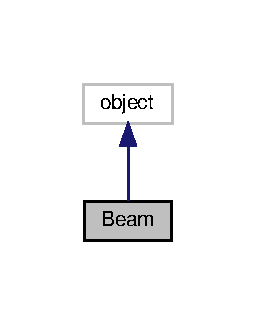
\includegraphics[width=123pt]{classpewpewlaz0rt4nk_1_1_beam__inherit__graph}
\end{center}
\end{figure}


Collaboration diagram for Beam\+:
\nopagebreak
\begin{figure}[H]
\begin{center}
\leavevmode
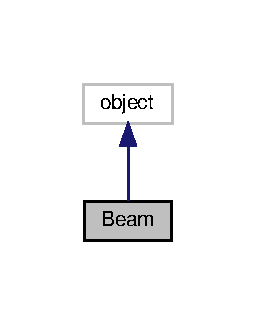
\includegraphics[width=123pt]{classpewpewlaz0rt4nk_1_1_beam__coll__graph}
\end{center}
\end{figure}
\subsection*{Public Member Functions}
\begin{DoxyCompactItemize}
\item 
def \hyperlink{classpewpewlaz0rt4nk_1_1_beam_ab990f1d831d1f24fff891d8726d10300}{\+\_\+\+\_\+init\+\_\+\+\_\+} (self, \hyperlink{classpewpewlaz0rt4nk_1_1_beam_a51e6a0d2bcb8531a5e5adcd66a77aa3b}{request}, \hyperlink{classpewpewlaz0rt4nk_1_1_beam_a8ab7bcb35ce5bba05608c72da6b4a0d3}{response}, \hyperlink{classpewpewlaz0rt4nk_1_1_beam_a2661f439a4a94ffdcd5e47ae1da0bb1d}{description}=None, \hyperlink{classpewpewlaz0rt4nk_1_1_beam_a832ddc04754e8a43d4f3c6165b1294a7}{host}=None, \hyperlink{classpewpewlaz0rt4nk_1_1_beam_af8fb0f45ee0195c7422a49e6a8d72369}{port}=None, \hyperlink{classpewpewlaz0rt4nk_1_1_beam_aee145bfca8e9b2eaf3cd3c47157be9a3}{timeout}=None, buffer\+\_\+=4096, \hyperlink{classpewpewlaz0rt4nk_1_1_beam_aa4a2d3facfe7f685ce8fdb8fdf68ac44}{shutdown}=False)
\item 
def \hyperlink{classpewpewlaz0rt4nk_1_1_beam_a51829b63adb24ac48d350dee60181002}{reset} (self)
\item 
def \hyperlink{classpewpewlaz0rt4nk_1_1_beam_a5505259a51131fe89dbde6fbeab32b52}{connect} (self)
\item 
def \hyperlink{classpewpewlaz0rt4nk_1_1_beam_a0fbdc6c4c08e0f205d671ea3cb6fffdd}{send} (self)
\item 
def \hyperlink{classpewpewlaz0rt4nk_1_1_beam_a06b2ff79fbf32e40f6f846b887ec7245}{receive} (self)
\item 
def \hyperlink{classpewpewlaz0rt4nk_1_1_beam_a00fe8c4d6cb42ed708b01611e4bc70dd}{shutdown\+\_\+socket} (self)
\item 
def \hyperlink{classpewpewlaz0rt4nk_1_1_beam_a7e676bc8e672824cf0719bff524d4067}{validate} (self)
\item 
def \hyperlink{classpewpewlaz0rt4nk_1_1_beam_a2561ec6ff5ec151676f3e0206e635bb8}{terminate} (self)
\end{DoxyCompactItemize}
\subsection*{Data Fields}
\begin{DoxyCompactItemize}
\item 
\hyperlink{classpewpewlaz0rt4nk_1_1_beam_a51e6a0d2bcb8531a5e5adcd66a77aa3b}{request}
\item 
\hyperlink{classpewpewlaz0rt4nk_1_1_beam_a8ab7bcb35ce5bba05608c72da6b4a0d3}{response}
\item 
\hyperlink{classpewpewlaz0rt4nk_1_1_beam_a2661f439a4a94ffdcd5e47ae1da0bb1d}{description}
\item 
\hyperlink{classpewpewlaz0rt4nk_1_1_beam_a832ddc04754e8a43d4f3c6165b1294a7}{host}
\item 
\hyperlink{classpewpewlaz0rt4nk_1_1_beam_af8fb0f45ee0195c7422a49e6a8d72369}{port}
\item 
\hyperlink{classpewpewlaz0rt4nk_1_1_beam_aee145bfca8e9b2eaf3cd3c47157be9a3}{timeout}
\item 
\hyperlink{classpewpewlaz0rt4nk_1_1_beam_a38acb51b2a63fccbafac9c0afca0c1b9}{buffer}
\item 
\hyperlink{classpewpewlaz0rt4nk_1_1_beam_aa4a2d3facfe7f685ce8fdb8fdf68ac44}{shutdown}
\end{DoxyCompactItemize}


\subsection{Detailed Description}
\begin{DoxyVerb}A beam to be shot by the :class:`Laz0rCannon` (e.g. an HTTP test case).

Arguments:
    - `request`: The request string that will be sent.
    - `response`: An iterable of strings containing the expected
      response.
    - `description`: The description of the test case.
    - `host`: The hostname of the HTTP server.
    - `port`: The port number where the HTTP server is reachable.
    - `timeout`: The amount of seconds until a timeout occurs while
       reading from/writing to the socket.
    - `buffer_`: The amount of bytes that will be sent at once. See
      :ref:`this section <buffer_>`.
    - `shutdown`: `False` or one of the constants of module
      :mod:`socket`. See :ref:`this section <shutdown>`.
\end{DoxyVerb}
 

\subsection{Constructor \& Destructor Documentation}
\mbox{\Hypertarget{classpewpewlaz0rt4nk_1_1_beam_ab990f1d831d1f24fff891d8726d10300}\label{classpewpewlaz0rt4nk_1_1_beam_ab990f1d831d1f24fff891d8726d10300}} 
\index{pewpewlaz0rt4nk\+::\+Beam@{pewpewlaz0rt4nk\+::\+Beam}!\+\_\+\+\_\+init\+\_\+\+\_\+@{\+\_\+\+\_\+init\+\_\+\+\_\+}}
\index{\+\_\+\+\_\+init\+\_\+\+\_\+@{\+\_\+\+\_\+init\+\_\+\+\_\+}!pewpewlaz0rt4nk\+::\+Beam@{pewpewlaz0rt4nk\+::\+Beam}}
\subsubsection{\texorpdfstring{\+\_\+\+\_\+init\+\_\+\+\_\+()}{\_\_init\_\_()}}
{\footnotesize\ttfamily def \+\_\+\+\_\+init\+\_\+\+\_\+ (\begin{DoxyParamCaption}\item[{}]{self,  }\item[{}]{request,  }\item[{}]{response,  }\item[{}]{description = {\ttfamily None},  }\item[{}]{host = {\ttfamily None},  }\item[{}]{port = {\ttfamily None},  }\item[{}]{timeout = {\ttfamily None},  }\item[{}]{buffer\+\_\+ = {\ttfamily 4096},  }\item[{}]{shutdown = {\ttfamily False} }\end{DoxyParamCaption})}

\begin{DoxyVerb}Initialize the beam and store the arguments\end{DoxyVerb}
 

\subsection{Member Function Documentation}
\mbox{\Hypertarget{classpewpewlaz0rt4nk_1_1_beam_a5505259a51131fe89dbde6fbeab32b52}\label{classpewpewlaz0rt4nk_1_1_beam_a5505259a51131fe89dbde6fbeab32b52}} 
\index{pewpewlaz0rt4nk\+::\+Beam@{pewpewlaz0rt4nk\+::\+Beam}!connect@{connect}}
\index{connect@{connect}!pewpewlaz0rt4nk\+::\+Beam@{pewpewlaz0rt4nk\+::\+Beam}}
\subsubsection{\texorpdfstring{connect()}{connect()}}
{\footnotesize\ttfamily def connect (\begin{DoxyParamCaption}\item[{}]{self }\end{DoxyParamCaption})}

\begin{DoxyVerb}Create a :mod:`socket` and establish a connection to the host.
\end{DoxyVerb}
 \mbox{\Hypertarget{classpewpewlaz0rt4nk_1_1_beam_a06b2ff79fbf32e40f6f846b887ec7245}\label{classpewpewlaz0rt4nk_1_1_beam_a06b2ff79fbf32e40f6f846b887ec7245}} 
\index{pewpewlaz0rt4nk\+::\+Beam@{pewpewlaz0rt4nk\+::\+Beam}!receive@{receive}}
\index{receive@{receive}!pewpewlaz0rt4nk\+::\+Beam@{pewpewlaz0rt4nk\+::\+Beam}}
\subsubsection{\texorpdfstring{receive()}{receive()}}
{\footnotesize\ttfamily def receive (\begin{DoxyParamCaption}\item[{}]{self }\end{DoxyParamCaption})}

\begin{DoxyVerb}Receive the HTTP response via an established connection.

Return the amount of calls to :meth:`~socket.socket.recv`.

Raises:
    - :class:`BeamRequestError`: The HTTP request has not been
      sent, yet.
    - :class:`BeamResponseError`: The HTTP response has already
      been received.
\end{DoxyVerb}
 \mbox{\Hypertarget{classpewpewlaz0rt4nk_1_1_beam_a51829b63adb24ac48d350dee60181002}\label{classpewpewlaz0rt4nk_1_1_beam_a51829b63adb24ac48d350dee60181002}} 
\index{pewpewlaz0rt4nk\+::\+Beam@{pewpewlaz0rt4nk\+::\+Beam}!reset@{reset}}
\index{reset@{reset}!pewpewlaz0rt4nk\+::\+Beam@{pewpewlaz0rt4nk\+::\+Beam}}
\subsubsection{\texorpdfstring{reset()}{reset()}}
{\footnotesize\ttfamily def reset (\begin{DoxyParamCaption}\item[{}]{self }\end{DoxyParamCaption})}

\begin{DoxyVerb}Reset attributes needed to reuse this beam.\end{DoxyVerb}
 \mbox{\Hypertarget{classpewpewlaz0rt4nk_1_1_beam_a0fbdc6c4c08e0f205d671ea3cb6fffdd}\label{classpewpewlaz0rt4nk_1_1_beam_a0fbdc6c4c08e0f205d671ea3cb6fffdd}} 
\index{pewpewlaz0rt4nk\+::\+Beam@{pewpewlaz0rt4nk\+::\+Beam}!send@{send}}
\index{send@{send}!pewpewlaz0rt4nk\+::\+Beam@{pewpewlaz0rt4nk\+::\+Beam}}
\subsubsection{\texorpdfstring{send()}{send()}}
{\footnotesize\ttfamily def send (\begin{DoxyParamCaption}\item[{}]{self }\end{DoxyParamCaption})}

\begin{DoxyVerb}Send the HTTP request via an established connection.

Return the amount of calls to :meth:`~socket.socket.send`.

Raises a :class:`BeamRequestError` if the request has already
been sent.
\end{DoxyVerb}
 \mbox{\Hypertarget{classpewpewlaz0rt4nk_1_1_beam_a00fe8c4d6cb42ed708b01611e4bc70dd}\label{classpewpewlaz0rt4nk_1_1_beam_a00fe8c4d6cb42ed708b01611e4bc70dd}} 
\index{pewpewlaz0rt4nk\+::\+Beam@{pewpewlaz0rt4nk\+::\+Beam}!shutdown\+\_\+socket@{shutdown\+\_\+socket}}
\index{shutdown\+\_\+socket@{shutdown\+\_\+socket}!pewpewlaz0rt4nk\+::\+Beam@{pewpewlaz0rt4nk\+::\+Beam}}
\subsubsection{\texorpdfstring{shutdown\+\_\+socket()}{shutdown\_socket()}}
{\footnotesize\ttfamily def shutdown\+\_\+socket (\begin{DoxyParamCaption}\item[{}]{self }\end{DoxyParamCaption})}

\begin{DoxyVerb}Shutdown the :mod:`socket` of an established connection.\end{DoxyVerb}
 \mbox{\Hypertarget{classpewpewlaz0rt4nk_1_1_beam_a2561ec6ff5ec151676f3e0206e635bb8}\label{classpewpewlaz0rt4nk_1_1_beam_a2561ec6ff5ec151676f3e0206e635bb8}} 
\index{pewpewlaz0rt4nk\+::\+Beam@{pewpewlaz0rt4nk\+::\+Beam}!terminate@{terminate}}
\index{terminate@{terminate}!pewpewlaz0rt4nk\+::\+Beam@{pewpewlaz0rt4nk\+::\+Beam}}
\subsubsection{\texorpdfstring{terminate()}{terminate()}}
{\footnotesize\ttfamily def terminate (\begin{DoxyParamCaption}\item[{}]{self }\end{DoxyParamCaption})}

\begin{DoxyVerb}Terminate an established connection to the :mod:`socket`.\end{DoxyVerb}
 \mbox{\Hypertarget{classpewpewlaz0rt4nk_1_1_beam_a7e676bc8e672824cf0719bff524d4067}\label{classpewpewlaz0rt4nk_1_1_beam_a7e676bc8e672824cf0719bff524d4067}} 
\index{pewpewlaz0rt4nk\+::\+Beam@{pewpewlaz0rt4nk\+::\+Beam}!validate@{validate}}
\index{validate@{validate}!pewpewlaz0rt4nk\+::\+Beam@{pewpewlaz0rt4nk\+::\+Beam}}
\subsubsection{\texorpdfstring{validate()}{validate()}}
{\footnotesize\ttfamily def validate (\begin{DoxyParamCaption}\item[{}]{self }\end{DoxyParamCaption})}

\begin{DoxyVerb}Validate an HTTP response.

Return a list of :class:`Response` instances.

Raises:
    - :class:`BeamRequestError`: The HTTP request has not been
      sent, yet.
    - :class:`BeamResponseError`: The HTTP response not been
      received, yet.
\end{DoxyVerb}
 

\subsection{Field Documentation}
\mbox{\Hypertarget{classpewpewlaz0rt4nk_1_1_beam_a38acb51b2a63fccbafac9c0afca0c1b9}\label{classpewpewlaz0rt4nk_1_1_beam_a38acb51b2a63fccbafac9c0afca0c1b9}} 
\index{pewpewlaz0rt4nk\+::\+Beam@{pewpewlaz0rt4nk\+::\+Beam}!buffer@{buffer}}
\index{buffer@{buffer}!pewpewlaz0rt4nk\+::\+Beam@{pewpewlaz0rt4nk\+::\+Beam}}
\subsubsection{\texorpdfstring{buffer}{buffer}}
{\footnotesize\ttfamily buffer}

\mbox{\Hypertarget{classpewpewlaz0rt4nk_1_1_beam_a2661f439a4a94ffdcd5e47ae1da0bb1d}\label{classpewpewlaz0rt4nk_1_1_beam_a2661f439a4a94ffdcd5e47ae1da0bb1d}} 
\index{pewpewlaz0rt4nk\+::\+Beam@{pewpewlaz0rt4nk\+::\+Beam}!description@{description}}
\index{description@{description}!pewpewlaz0rt4nk\+::\+Beam@{pewpewlaz0rt4nk\+::\+Beam}}
\subsubsection{\texorpdfstring{description}{description}}
{\footnotesize\ttfamily description}

\mbox{\Hypertarget{classpewpewlaz0rt4nk_1_1_beam_a832ddc04754e8a43d4f3c6165b1294a7}\label{classpewpewlaz0rt4nk_1_1_beam_a832ddc04754e8a43d4f3c6165b1294a7}} 
\index{pewpewlaz0rt4nk\+::\+Beam@{pewpewlaz0rt4nk\+::\+Beam}!host@{host}}
\index{host@{host}!pewpewlaz0rt4nk\+::\+Beam@{pewpewlaz0rt4nk\+::\+Beam}}
\subsubsection{\texorpdfstring{host}{host}}
{\footnotesize\ttfamily host}

\mbox{\Hypertarget{classpewpewlaz0rt4nk_1_1_beam_af8fb0f45ee0195c7422a49e6a8d72369}\label{classpewpewlaz0rt4nk_1_1_beam_af8fb0f45ee0195c7422a49e6a8d72369}} 
\index{pewpewlaz0rt4nk\+::\+Beam@{pewpewlaz0rt4nk\+::\+Beam}!port@{port}}
\index{port@{port}!pewpewlaz0rt4nk\+::\+Beam@{pewpewlaz0rt4nk\+::\+Beam}}
\subsubsection{\texorpdfstring{port}{port}}
{\footnotesize\ttfamily port}

\mbox{\Hypertarget{classpewpewlaz0rt4nk_1_1_beam_a51e6a0d2bcb8531a5e5adcd66a77aa3b}\label{classpewpewlaz0rt4nk_1_1_beam_a51e6a0d2bcb8531a5e5adcd66a77aa3b}} 
\index{pewpewlaz0rt4nk\+::\+Beam@{pewpewlaz0rt4nk\+::\+Beam}!request@{request}}
\index{request@{request}!pewpewlaz0rt4nk\+::\+Beam@{pewpewlaz0rt4nk\+::\+Beam}}
\subsubsection{\texorpdfstring{request}{request}}
{\footnotesize\ttfamily request}

\mbox{\Hypertarget{classpewpewlaz0rt4nk_1_1_beam_a8ab7bcb35ce5bba05608c72da6b4a0d3}\label{classpewpewlaz0rt4nk_1_1_beam_a8ab7bcb35ce5bba05608c72da6b4a0d3}} 
\index{pewpewlaz0rt4nk\+::\+Beam@{pewpewlaz0rt4nk\+::\+Beam}!response@{response}}
\index{response@{response}!pewpewlaz0rt4nk\+::\+Beam@{pewpewlaz0rt4nk\+::\+Beam}}
\subsubsection{\texorpdfstring{response}{response}}
{\footnotesize\ttfamily response}

\mbox{\Hypertarget{classpewpewlaz0rt4nk_1_1_beam_aa4a2d3facfe7f685ce8fdb8fdf68ac44}\label{classpewpewlaz0rt4nk_1_1_beam_aa4a2d3facfe7f685ce8fdb8fdf68ac44}} 
\index{pewpewlaz0rt4nk\+::\+Beam@{pewpewlaz0rt4nk\+::\+Beam}!shutdown@{shutdown}}
\index{shutdown@{shutdown}!pewpewlaz0rt4nk\+::\+Beam@{pewpewlaz0rt4nk\+::\+Beam}}
\subsubsection{\texorpdfstring{shutdown}{shutdown}}
{\footnotesize\ttfamily shutdown}

\mbox{\Hypertarget{classpewpewlaz0rt4nk_1_1_beam_aee145bfca8e9b2eaf3cd3c47157be9a3}\label{classpewpewlaz0rt4nk_1_1_beam_aee145bfca8e9b2eaf3cd3c47157be9a3}} 
\index{pewpewlaz0rt4nk\+::\+Beam@{pewpewlaz0rt4nk\+::\+Beam}!timeout@{timeout}}
\index{timeout@{timeout}!pewpewlaz0rt4nk\+::\+Beam@{pewpewlaz0rt4nk\+::\+Beam}}
\subsubsection{\texorpdfstring{timeout}{timeout}}
{\footnotesize\ttfamily timeout}



The documentation for this class was generated from the following file\+:\begin{DoxyCompactItemize}
\item 
\hyperlink{pewpewlaz0rt4nk_8py}{pewpewlaz0rt4nk.\+py}\end{DoxyCompactItemize}

\hypertarget{classpewpewlaz0rt4nk_1_1_beam_error}{}\section{Beam\+Error Class Reference}
\label{classpewpewlaz0rt4nk_1_1_beam_error}\index{Beam\+Error@{Beam\+Error}}


Inheritance diagram for Beam\+Error\+:
\nopagebreak
\begin{figure}[H]
\begin{center}
\leavevmode
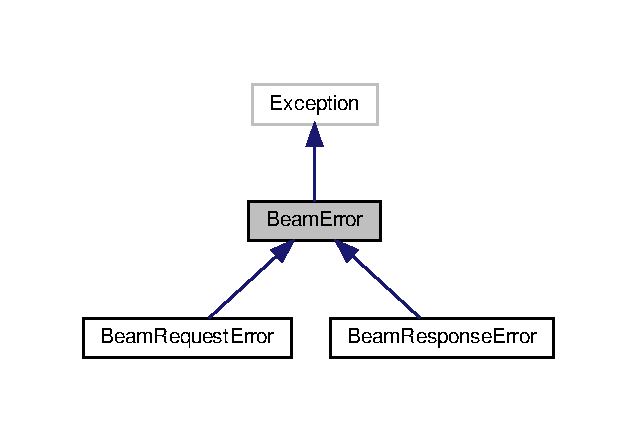
\includegraphics[width=306pt]{classpewpewlaz0rt4nk_1_1_beam_error__inherit__graph}
\end{center}
\end{figure}


Collaboration diagram for Beam\+Error\+:
\nopagebreak
\begin{figure}[H]
\begin{center}
\leavevmode
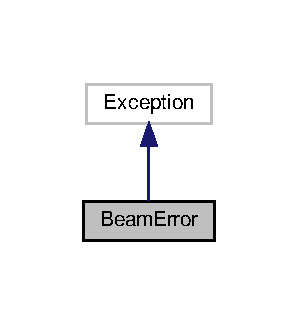
\includegraphics[width=143pt]{classpewpewlaz0rt4nk_1_1_beam_error__coll__graph}
\end{center}
\end{figure}


\subsection{Detailed Description}
\begin{DoxyVerb}This exception is for uncategorised beam errors.\end{DoxyVerb}
 

The documentation for this class was generated from the following file\+:\begin{DoxyCompactItemize}
\item 
\hyperlink{pewpewlaz0rt4nk_8py}{pewpewlaz0rt4nk.\+py}\end{DoxyCompactItemize}

\hypertarget{classpewpewlaz0rt4nk_1_1_beam_request_error}{}\section{Beam\+Request\+Error Class Reference}
\label{classpewpewlaz0rt4nk_1_1_beam_request_error}\index{Beam\+Request\+Error@{Beam\+Request\+Error}}


Inheritance diagram for Beam\+Request\+Error\+:
\nopagebreak
\begin{figure}[H]
\begin{center}
\leavevmode
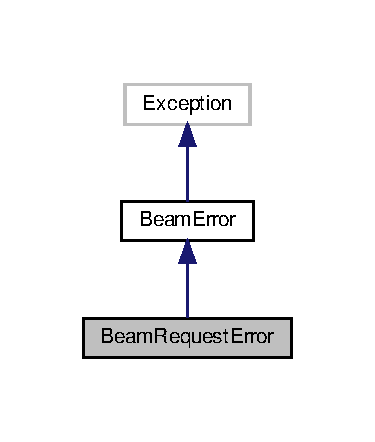
\includegraphics[width=180pt]{classpewpewlaz0rt4nk_1_1_beam_request_error__inherit__graph}
\end{center}
\end{figure}


Collaboration diagram for Beam\+Request\+Error\+:
\nopagebreak
\begin{figure}[H]
\begin{center}
\leavevmode
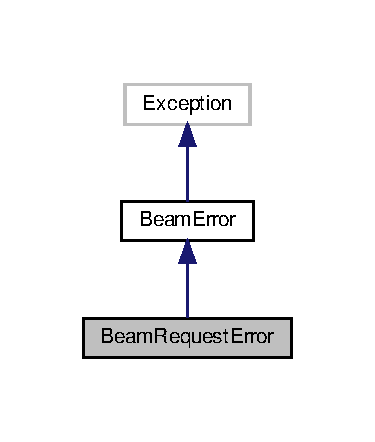
\includegraphics[width=180pt]{classpewpewlaz0rt4nk_1_1_beam_request_error__coll__graph}
\end{center}
\end{figure}


\subsection{Detailed Description}
\begin{DoxyVerb}This exception is for HTTP request related errors.\end{DoxyVerb}
 

The documentation for this class was generated from the following file\+:\begin{DoxyCompactItemize}
\item 
\hyperlink{pewpewlaz0rt4nk_8py}{pewpewlaz0rt4nk.\+py}\end{DoxyCompactItemize}

\hypertarget{classpewpewlaz0rt4nk_1_1_beam_response_error}{}\section{Beam\+Response\+Error Class Reference}
\label{classpewpewlaz0rt4nk_1_1_beam_response_error}\index{Beam\+Response\+Error@{Beam\+Response\+Error}}


Inheritance diagram for Beam\+Response\+Error\+:
\nopagebreak
\begin{figure}[H]
\begin{center}
\leavevmode
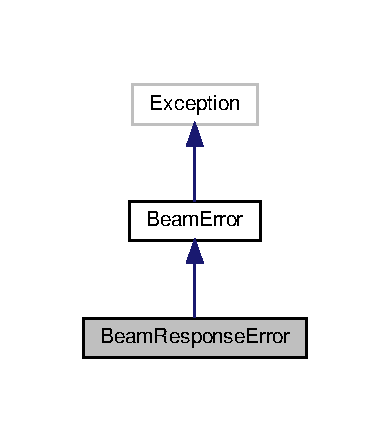
\includegraphics[width=187pt]{classpewpewlaz0rt4nk_1_1_beam_response_error__inherit__graph}
\end{center}
\end{figure}


Collaboration diagram for Beam\+Response\+Error\+:
\nopagebreak
\begin{figure}[H]
\begin{center}
\leavevmode
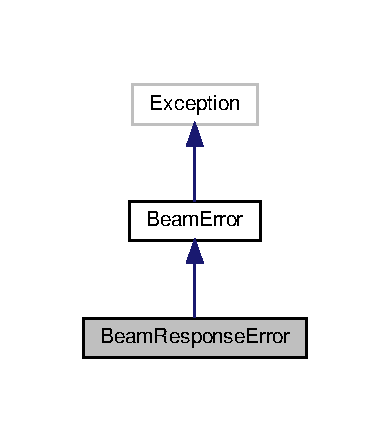
\includegraphics[width=187pt]{classpewpewlaz0rt4nk_1_1_beam_response_error__coll__graph}
\end{center}
\end{figure}


\subsection{Detailed Description}
\begin{DoxyVerb}This exception is for HTTP response related errors.\end{DoxyVerb}
 

The documentation for this class was generated from the following file\+:\begin{DoxyCompactItemize}
\item 
\hyperlink{pewpewlaz0rt4nk_8py}{pewpewlaz0rt4nk.\+py}\end{DoxyCompactItemize}

\hypertarget{structhttp__request__struct}{}\section{http\+\_\+request\+\_\+struct Struct Reference}
\label{structhttp__request__struct}\index{http\+\_\+request\+\_\+struct@{http\+\_\+request\+\_\+struct}}


{\ttfamily \#include $<$request.\+h$>$}



Collaboration diagram for http\+\_\+request\+\_\+struct\+:
\nopagebreak
\begin{figure}[H]
\begin{center}
\leavevmode
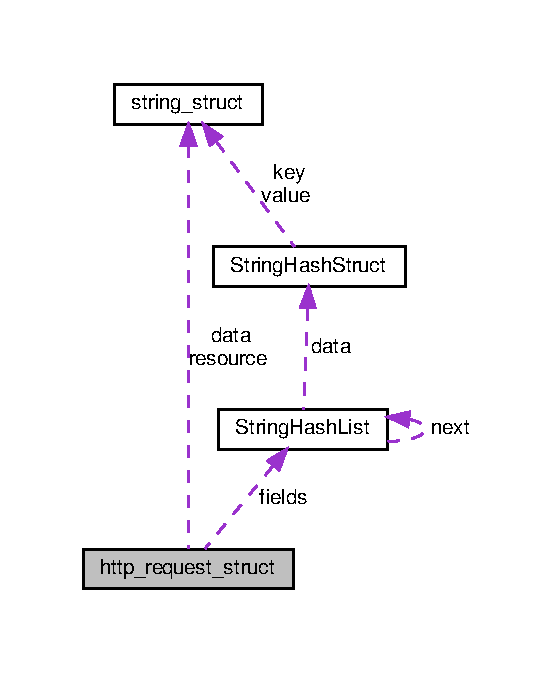
\includegraphics[width=266pt]{structhttp__request__struct__coll__graph}
\end{center}
\end{figure}
\subsection*{Data Fields}
\begin{DoxyCompactItemize}
\item 
\hyperlink{helpers_8h_a837a089a977b319a11edfb8022d9e47d}{H\+T\+T\+P\+Method} \hyperlink{structhttp__request__struct_a142613365447813080ed707830788a63}{method}
\item 
\hyperlink{string_8h_a3d2981d9da3e25dd89371059777fdd12}{string} $\ast$ \hyperlink{structhttp__request__struct_a09aa4e1a1b2609255ee841c0607d8bea}{resource}
\item 
\hyperlink{helpers_8h_abe818f5ff14e9c60c052a3e96877cec6}{H\+T\+T\+P\+Version} \hyperlink{structhttp__request__struct_ad3e7ead879a6e870226227ac79d73ec9}{version}
\item 
\hyperlink{hash_8h_a58bb615f9115c5b9b1a49a64d3737edf}{Hash\+List} $\ast$ \hyperlink{structhttp__request__struct_a640c838701b686459e80b063a9604a7c}{fields}
\item 
\hyperlink{string_8h_a3d2981d9da3e25dd89371059777fdd12}{string} $\ast$ \hyperlink{structhttp__request__struct_af9e4d83beef89b79bf9a9c0c7f00ddcc}{data}
\end{DoxyCompactItemize}


\subsection{Field Documentation}
\mbox{\Hypertarget{structhttp__request__struct_af9e4d83beef89b79bf9a9c0c7f00ddcc}\label{structhttp__request__struct_af9e4d83beef89b79bf9a9c0c7f00ddcc}} 
\index{http\+\_\+request\+\_\+struct@{http\+\_\+request\+\_\+struct}!data@{data}}
\index{data@{data}!http\+\_\+request\+\_\+struct@{http\+\_\+request\+\_\+struct}}
\subsubsection{\texorpdfstring{data}{data}}
{\footnotesize\ttfamily \hyperlink{string_8h_a3d2981d9da3e25dd89371059777fdd12}{string}$\ast$ data}

\mbox{\Hypertarget{structhttp__request__struct_a640c838701b686459e80b063a9604a7c}\label{structhttp__request__struct_a640c838701b686459e80b063a9604a7c}} 
\index{http\+\_\+request\+\_\+struct@{http\+\_\+request\+\_\+struct}!fields@{fields}}
\index{fields@{fields}!http\+\_\+request\+\_\+struct@{http\+\_\+request\+\_\+struct}}
\subsubsection{\texorpdfstring{fields}{fields}}
{\footnotesize\ttfamily \hyperlink{hash_8h_a58bb615f9115c5b9b1a49a64d3737edf}{Hash\+List}$\ast$ fields}

\mbox{\Hypertarget{structhttp__request__struct_a142613365447813080ed707830788a63}\label{structhttp__request__struct_a142613365447813080ed707830788a63}} 
\index{http\+\_\+request\+\_\+struct@{http\+\_\+request\+\_\+struct}!method@{method}}
\index{method@{method}!http\+\_\+request\+\_\+struct@{http\+\_\+request\+\_\+struct}}
\subsubsection{\texorpdfstring{method}{method}}
{\footnotesize\ttfamily \hyperlink{helpers_8h_a837a089a977b319a11edfb8022d9e47d}{H\+T\+T\+P\+Method} method}

\mbox{\Hypertarget{structhttp__request__struct_a09aa4e1a1b2609255ee841c0607d8bea}\label{structhttp__request__struct_a09aa4e1a1b2609255ee841c0607d8bea}} 
\index{http\+\_\+request\+\_\+struct@{http\+\_\+request\+\_\+struct}!resource@{resource}}
\index{resource@{resource}!http\+\_\+request\+\_\+struct@{http\+\_\+request\+\_\+struct}}
\subsubsection{\texorpdfstring{resource}{resource}}
{\footnotesize\ttfamily \hyperlink{string_8h_a3d2981d9da3e25dd89371059777fdd12}{string}$\ast$ resource}

\mbox{\Hypertarget{structhttp__request__struct_ad3e7ead879a6e870226227ac79d73ec9}\label{structhttp__request__struct_ad3e7ead879a6e870226227ac79d73ec9}} 
\index{http\+\_\+request\+\_\+struct@{http\+\_\+request\+\_\+struct}!version@{version}}
\index{version@{version}!http\+\_\+request\+\_\+struct@{http\+\_\+request\+\_\+struct}}
\subsubsection{\texorpdfstring{version}{version}}
{\footnotesize\ttfamily \hyperlink{helpers_8h_abe818f5ff14e9c60c052a3e96877cec6}{H\+T\+T\+P\+Version} version}



The documentation for this struct was generated from the following file\+:\begin{DoxyCompactItemize}
\item 
\hyperlink{request_8h}{request.\+h}\end{DoxyCompactItemize}

\hypertarget{classpewpewlaz0rt4nk_1_1_laz0r_cannon}{}\section{Laz0r\+Cannon Class Reference}
\label{classpewpewlaz0rt4nk_1_1_laz0r_cannon}\index{Laz0r\+Cannon@{Laz0r\+Cannon}}


Inheritance diagram for Laz0r\+Cannon\+:
\nopagebreak
\begin{figure}[H]
\begin{center}
\leavevmode
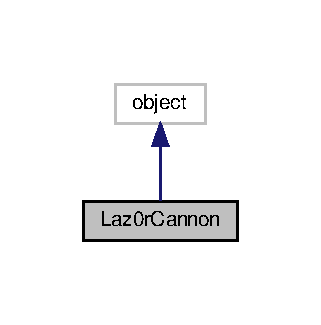
\includegraphics[width=154pt]{classpewpewlaz0rt4nk_1_1_laz0r_cannon__inherit__graph}
\end{center}
\end{figure}


Collaboration diagram for Laz0r\+Cannon\+:
\nopagebreak
\begin{figure}[H]
\begin{center}
\leavevmode
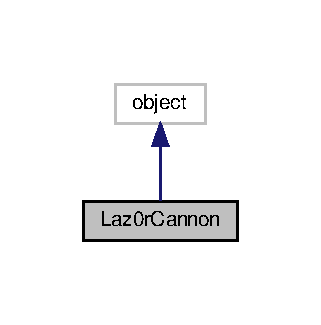
\includegraphics[width=154pt]{classpewpewlaz0rt4nk_1_1_laz0r_cannon__coll__graph}
\end{center}
\end{figure}
\subsection*{Public Member Functions}
\begin{DoxyCompactItemize}
\item 
def \hyperlink{classpewpewlaz0rt4nk_1_1_laz0r_cannon_a3dd756910e3c6b07498f060bdf0b417e}{\+\_\+\+\_\+init\+\_\+\+\_\+} (self, host=None, port=None, timeout=3, use\+\_\+colors=True)
\item 
def \hyperlink{classpewpewlaz0rt4nk_1_1_laz0r_cannon_a51829b63adb24ac48d350dee60181002}{reset} (self)
\item 
def \hyperlink{classpewpewlaz0rt4nk_1_1_laz0r_cannon_a95d2c7f7c4173d33f1a2b9f70544f6fb}{add} (self, beam)
\item 
def \hyperlink{classpewpewlaz0rt4nk_1_1_laz0r_cannon_ada8f9d781d3eb083a027b074306d85db}{\+\_\+\+\_\+iadd\+\_\+\+\_\+} (self, beam)
\item 
def \hyperlink{classpewpewlaz0rt4nk_1_1_laz0r_cannon_a602db2841c236b79433716f61c5e2d01}{pewpew} (self, settings=True)
\end{DoxyCompactItemize}


\subsection{Detailed Description}
\begin{DoxyVerb}A laz0r cannon that shoots laz0r beams at HTTP servers.

Arguments:
    - `host`: The hostname of the HTTP server.
    - `port`: The port number where the HTTP server is reachable.
    - `timeout`: The amount of seconds until a timeout occurs while
      reading from/writing to the socket.
    - `use_colors`: Turn colored output on the console on or off.
\end{DoxyVerb}
 

\subsection{Constructor \& Destructor Documentation}
\mbox{\Hypertarget{classpewpewlaz0rt4nk_1_1_laz0r_cannon_a3dd756910e3c6b07498f060bdf0b417e}\label{classpewpewlaz0rt4nk_1_1_laz0r_cannon_a3dd756910e3c6b07498f060bdf0b417e}} 
\index{pewpewlaz0rt4nk\+::\+Laz0r\+Cannon@{pewpewlaz0rt4nk\+::\+Laz0r\+Cannon}!\+\_\+\+\_\+init\+\_\+\+\_\+@{\+\_\+\+\_\+init\+\_\+\+\_\+}}
\index{\+\_\+\+\_\+init\+\_\+\+\_\+@{\+\_\+\+\_\+init\+\_\+\+\_\+}!pewpewlaz0rt4nk\+::\+Laz0r\+Cannon@{pewpewlaz0rt4nk\+::\+Laz0r\+Cannon}}
\subsubsection{\texorpdfstring{\+\_\+\+\_\+init\+\_\+\+\_\+()}{\_\_init\_\_()}}
{\footnotesize\ttfamily def \+\_\+\+\_\+init\+\_\+\+\_\+ (\begin{DoxyParamCaption}\item[{}]{self,  }\item[{}]{host = {\ttfamily None},  }\item[{}]{port = {\ttfamily None},  }\item[{}]{timeout = {\ttfamily 3},  }\item[{}]{use\+\_\+colors = {\ttfamily True} }\end{DoxyParamCaption})}

\begin{DoxyVerb}Initialize the laz0r cannon and store the arguments.\end{DoxyVerb}
 

\subsection{Member Function Documentation}
\mbox{\Hypertarget{classpewpewlaz0rt4nk_1_1_laz0r_cannon_ada8f9d781d3eb083a027b074306d85db}\label{classpewpewlaz0rt4nk_1_1_laz0r_cannon_ada8f9d781d3eb083a027b074306d85db}} 
\index{pewpewlaz0rt4nk\+::\+Laz0r\+Cannon@{pewpewlaz0rt4nk\+::\+Laz0r\+Cannon}!\+\_\+\+\_\+iadd\+\_\+\+\_\+@{\+\_\+\+\_\+iadd\+\_\+\+\_\+}}
\index{\+\_\+\+\_\+iadd\+\_\+\+\_\+@{\+\_\+\+\_\+iadd\+\_\+\+\_\+}!pewpewlaz0rt4nk\+::\+Laz0r\+Cannon@{pewpewlaz0rt4nk\+::\+Laz0r\+Cannon}}
\subsubsection{\texorpdfstring{\+\_\+\+\_\+iadd\+\_\+\+\_\+()}{\_\_iadd\_\_()}}
{\footnotesize\ttfamily def \+\_\+\+\_\+iadd\+\_\+\+\_\+ (\begin{DoxyParamCaption}\item[{}]{self,  }\item[{}]{beam }\end{DoxyParamCaption})}

\begin{DoxyVerb}Add a beam to the cannon with style.\end{DoxyVerb}
 \mbox{\Hypertarget{classpewpewlaz0rt4nk_1_1_laz0r_cannon_a95d2c7f7c4173d33f1a2b9f70544f6fb}\label{classpewpewlaz0rt4nk_1_1_laz0r_cannon_a95d2c7f7c4173d33f1a2b9f70544f6fb}} 
\index{pewpewlaz0rt4nk\+::\+Laz0r\+Cannon@{pewpewlaz0rt4nk\+::\+Laz0r\+Cannon}!add@{add}}
\index{add@{add}!pewpewlaz0rt4nk\+::\+Laz0r\+Cannon@{pewpewlaz0rt4nk\+::\+Laz0r\+Cannon}}
\subsubsection{\texorpdfstring{add()}{add()}}
{\footnotesize\ttfamily def add (\begin{DoxyParamCaption}\item[{}]{self,  }\item[{}]{beam }\end{DoxyParamCaption})}

\begin{DoxyVerb}Add a beam to the cannon.

Arguments:
    - `beam`: A :class:`Beam` instance.

The attributes `host`, `port` and `timeout` of a :class:`Beam`
will be overwritten by this class's attributes if they haven't
been defined explicitly.
\end{DoxyVerb}
 \mbox{\Hypertarget{classpewpewlaz0rt4nk_1_1_laz0r_cannon_a602db2841c236b79433716f61c5e2d01}\label{classpewpewlaz0rt4nk_1_1_laz0r_cannon_a602db2841c236b79433716f61c5e2d01}} 
\index{pewpewlaz0rt4nk\+::\+Laz0r\+Cannon@{pewpewlaz0rt4nk\+::\+Laz0r\+Cannon}!pewpew@{pewpew}}
\index{pewpew@{pewpew}!pewpewlaz0rt4nk\+::\+Laz0r\+Cannon@{pewpewlaz0rt4nk\+::\+Laz0r\+Cannon}}
\subsubsection{\texorpdfstring{pewpew()}{pewpew()}}
{\footnotesize\ttfamily def pewpew (\begin{DoxyParamCaption}\item[{}]{self,  }\item[{}]{settings = {\ttfamily True} }\end{DoxyParamCaption})}

\begin{DoxyVerb}Align the laz0r cannon and `PEWPEWs` each laz0r :class:`Beam`
towards the HTTP server.

Arguments:
    - `settings`: If set to `True` setting informations will be
      printed.
\end{DoxyVerb}
 \mbox{\Hypertarget{classpewpewlaz0rt4nk_1_1_laz0r_cannon_a51829b63adb24ac48d350dee60181002}\label{classpewpewlaz0rt4nk_1_1_laz0r_cannon_a51829b63adb24ac48d350dee60181002}} 
\index{pewpewlaz0rt4nk\+::\+Laz0r\+Cannon@{pewpewlaz0rt4nk\+::\+Laz0r\+Cannon}!reset@{reset}}
\index{reset@{reset}!pewpewlaz0rt4nk\+::\+Laz0r\+Cannon@{pewpewlaz0rt4nk\+::\+Laz0r\+Cannon}}
\subsubsection{\texorpdfstring{reset()}{reset()}}
{\footnotesize\ttfamily def reset (\begin{DoxyParamCaption}\item[{}]{self }\end{DoxyParamCaption})}

\begin{DoxyVerb}Reset statistics of passed and failed HTTP responses.\end{DoxyVerb}
 

The documentation for this class was generated from the following file\+:\begin{DoxyCompactItemize}
\item 
\hyperlink{pewpewlaz0rt4nk_8py}{pewpewlaz0rt4nk.\+py}\end{DoxyCompactItemize}

\hypertarget{classpewpewlaz0rt4nk_1_1_response}{}\section{Response Class Reference}
\label{classpewpewlaz0rt4nk_1_1_response}\index{Response@{Response}}


Inheritance diagram for Response\+:
\nopagebreak
\begin{figure}[H]
\begin{center}
\leavevmode
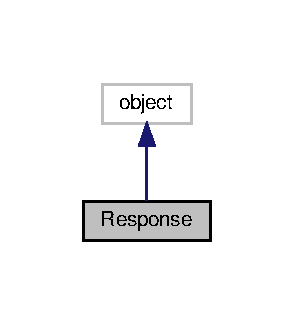
\includegraphics[width=141pt]{classpewpewlaz0rt4nk_1_1_response__inherit__graph}
\end{center}
\end{figure}


Collaboration diagram for Response\+:
\nopagebreak
\begin{figure}[H]
\begin{center}
\leavevmode
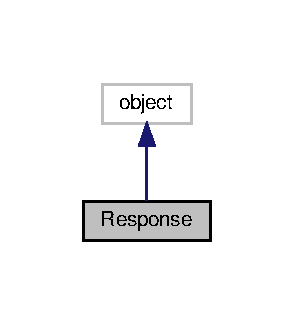
\includegraphics[width=141pt]{classpewpewlaz0rt4nk_1_1_response__coll__graph}
\end{center}
\end{figure}
\subsection*{Public Member Functions}
\begin{DoxyCompactItemize}
\item 
def \hyperlink{classpewpewlaz0rt4nk_1_1_response_aba15f6a5c8c7934fc61604b13ebb85a8}{\+\_\+\+\_\+init\+\_\+\+\_\+} (self, \hyperlink{classpewpewlaz0rt4nk_1_1_response_a40c180ffecdf131ba12f6a09349a1033}{pass\+\_\+}, \hyperlink{classpewpewlaz0rt4nk_1_1_response_aa6e67bddae371a5731f6d4002e787299}{expected}, \hyperlink{classpewpewlaz0rt4nk_1_1_response_a082fd9f55493d749cafc1e11ad84a2b6}{received})
\end{DoxyCompactItemize}
\subsection*{Data Fields}
\begin{DoxyCompactItemize}
\item 
\hyperlink{classpewpewlaz0rt4nk_1_1_response_a40c180ffecdf131ba12f6a09349a1033}{pass\+\_\+}
\item 
\hyperlink{classpewpewlaz0rt4nk_1_1_response_aa6e67bddae371a5731f6d4002e787299}{expected}
\item 
\hyperlink{classpewpewlaz0rt4nk_1_1_response_a082fd9f55493d749cafc1e11ad84a2b6}{received}
\end{DoxyCompactItemize}


\subsection{Detailed Description}
\begin{DoxyVerb}Container to store a validated HTTP response line.

Arguments:
    - `pass_`: Represents a valid or invalid response line.
    - `expected`: The expected response string.
    - `received`: The actual response string.
\end{DoxyVerb}
 

\subsection{Constructor \& Destructor Documentation}
\mbox{\Hypertarget{classpewpewlaz0rt4nk_1_1_response_aba15f6a5c8c7934fc61604b13ebb85a8}\label{classpewpewlaz0rt4nk_1_1_response_aba15f6a5c8c7934fc61604b13ebb85a8}} 
\index{pewpewlaz0rt4nk\+::\+Response@{pewpewlaz0rt4nk\+::\+Response}!\+\_\+\+\_\+init\+\_\+\+\_\+@{\+\_\+\+\_\+init\+\_\+\+\_\+}}
\index{\+\_\+\+\_\+init\+\_\+\+\_\+@{\+\_\+\+\_\+init\+\_\+\+\_\+}!pewpewlaz0rt4nk\+::\+Response@{pewpewlaz0rt4nk\+::\+Response}}
\subsubsection{\texorpdfstring{\+\_\+\+\_\+init\+\_\+\+\_\+()}{\_\_init\_\_()}}
{\footnotesize\ttfamily def \+\_\+\+\_\+init\+\_\+\+\_\+ (\begin{DoxyParamCaption}\item[{}]{self,  }\item[{}]{pass\+\_\+,  }\item[{}]{expected,  }\item[{}]{received }\end{DoxyParamCaption})}

\begin{DoxyVerb}Initialize the container and store the arguments.\end{DoxyVerb}
 

\subsection{Field Documentation}
\mbox{\Hypertarget{classpewpewlaz0rt4nk_1_1_response_aa6e67bddae371a5731f6d4002e787299}\label{classpewpewlaz0rt4nk_1_1_response_aa6e67bddae371a5731f6d4002e787299}} 
\index{pewpewlaz0rt4nk\+::\+Response@{pewpewlaz0rt4nk\+::\+Response}!expected@{expected}}
\index{expected@{expected}!pewpewlaz0rt4nk\+::\+Response@{pewpewlaz0rt4nk\+::\+Response}}
\subsubsection{\texorpdfstring{expected}{expected}}
{\footnotesize\ttfamily expected}

\mbox{\Hypertarget{classpewpewlaz0rt4nk_1_1_response_a40c180ffecdf131ba12f6a09349a1033}\label{classpewpewlaz0rt4nk_1_1_response_a40c180ffecdf131ba12f6a09349a1033}} 
\index{pewpewlaz0rt4nk\+::\+Response@{pewpewlaz0rt4nk\+::\+Response}!pass\+\_\+@{pass\+\_\+}}
\index{pass\+\_\+@{pass\+\_\+}!pewpewlaz0rt4nk\+::\+Response@{pewpewlaz0rt4nk\+::\+Response}}
\subsubsection{\texorpdfstring{pass\+\_\+}{pass\_}}
{\footnotesize\ttfamily pass\+\_\+}

\mbox{\Hypertarget{classpewpewlaz0rt4nk_1_1_response_a082fd9f55493d749cafc1e11ad84a2b6}\label{classpewpewlaz0rt4nk_1_1_response_a082fd9f55493d749cafc1e11ad84a2b6}} 
\index{pewpewlaz0rt4nk\+::\+Response@{pewpewlaz0rt4nk\+::\+Response}!received@{received}}
\index{received@{received}!pewpewlaz0rt4nk\+::\+Response@{pewpewlaz0rt4nk\+::\+Response}}
\subsubsection{\texorpdfstring{received}{received}}
{\footnotesize\ttfamily received}



The documentation for this class was generated from the following file\+:\begin{DoxyCompactItemize}
\item 
\hyperlink{pewpewlaz0rt4nk_8py}{pewpewlaz0rt4nk.\+py}\end{DoxyCompactItemize}

\hypertarget{structstring__struct}{}\section{string\+\_\+struct Struct Reference}
\label{structstring__struct}\index{string\+\_\+struct@{string\+\_\+struct}}


{\ttfamily \#include $<$string.\+h$>$}

\subsection*{Data Fields}
\begin{DoxyCompactItemize}
\item 
size\+\_\+t \hyperlink{structstring__struct_ad721fc6ca6a3d6ba3bc506576622aab0}{capacity}
\item 
size\+\_\+t \hyperlink{structstring__struct_a7360b55975153b822efc5217b7734e6a}{len}
\item 
char $\ast$ \hyperlink{structstring__struct_a1fe855c208bc17a51a4d34fefdb2d5b1}{buf}
\end{DoxyCompactItemize}


\subsection{Field Documentation}
\mbox{\Hypertarget{structstring__struct_a1fe855c208bc17a51a4d34fefdb2d5b1}\label{structstring__struct_a1fe855c208bc17a51a4d34fefdb2d5b1}} 
\index{string\+\_\+struct@{string\+\_\+struct}!buf@{buf}}
\index{buf@{buf}!string\+\_\+struct@{string\+\_\+struct}}
\subsubsection{\texorpdfstring{buf}{buf}}
{\footnotesize\ttfamily char$\ast$ buf}

\mbox{\Hypertarget{structstring__struct_ad721fc6ca6a3d6ba3bc506576622aab0}\label{structstring__struct_ad721fc6ca6a3d6ba3bc506576622aab0}} 
\index{string\+\_\+struct@{string\+\_\+struct}!capacity@{capacity}}
\index{capacity@{capacity}!string\+\_\+struct@{string\+\_\+struct}}
\subsubsection{\texorpdfstring{capacity}{capacity}}
{\footnotesize\ttfamily size\+\_\+t capacity}

\mbox{\Hypertarget{structstring__struct_a7360b55975153b822efc5217b7734e6a}\label{structstring__struct_a7360b55975153b822efc5217b7734e6a}} 
\index{string\+\_\+struct@{string\+\_\+struct}!len@{len}}
\index{len@{len}!string\+\_\+struct@{string\+\_\+struct}}
\subsubsection{\texorpdfstring{len}{len}}
{\footnotesize\ttfamily size\+\_\+t len}



The documentation for this struct was generated from the following file\+:\begin{DoxyCompactItemize}
\item 
\hyperlink{string_8h}{string.\+h}\end{DoxyCompactItemize}

\hypertarget{struct_string_hash_list}{}\section{String\+Hash\+List Struct Reference}
\label{struct_string_hash_list}\index{String\+Hash\+List@{String\+Hash\+List}}


Structure defining a list\+Element.  




{\ttfamily \#include $<$hash.\+h$>$}



Collaboration diagram for String\+Hash\+List\+:
\nopagebreak
\begin{figure}[H]
\begin{center}
\leavevmode
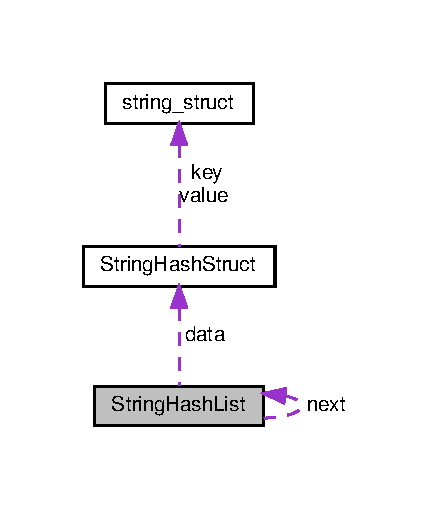
\includegraphics[width=207pt]{struct_string_hash_list__coll__graph}
\end{center}
\end{figure}
\subsection*{Data Fields}
\begin{DoxyCompactItemize}
\item 
\hyperlink{hash_8h_aaae8e320515f4ba6ab5e8bc4ecd7f58a}{Hash} \hyperlink{struct_string_hash_list_a0bb0e5ff64b92afb24dffc5a8835c55d}{data}
\begin{DoxyCompactList}\small\item\em Hash value of list element. \end{DoxyCompactList}\item 
struct \hyperlink{struct_string_hash_list}{String\+Hash\+List} $\ast$ \hyperlink{struct_string_hash_list_a61c5f91e0504062e5408438d1a3c1e78}{next}
\begin{DoxyCompactList}\small\item\em next list element \end{DoxyCompactList}\end{DoxyCompactItemize}


\subsection{Detailed Description}
Structure defining a list\+Element. 

\begin{DoxyAuthor}{Author}
Björn Marx 
\end{DoxyAuthor}


\subsection{Field Documentation}
\mbox{\Hypertarget{struct_string_hash_list_a0bb0e5ff64b92afb24dffc5a8835c55d}\label{struct_string_hash_list_a0bb0e5ff64b92afb24dffc5a8835c55d}} 
\index{String\+Hash\+List@{String\+Hash\+List}!data@{data}}
\index{data@{data}!String\+Hash\+List@{String\+Hash\+List}}
\subsubsection{\texorpdfstring{data}{data}}
{\footnotesize\ttfamily \hyperlink{hash_8h_aaae8e320515f4ba6ab5e8bc4ecd7f58a}{Hash} data}



Hash value of list element. 

\mbox{\Hypertarget{struct_string_hash_list_a61c5f91e0504062e5408438d1a3c1e78}\label{struct_string_hash_list_a61c5f91e0504062e5408438d1a3c1e78}} 
\index{String\+Hash\+List@{String\+Hash\+List}!next@{next}}
\index{next@{next}!String\+Hash\+List@{String\+Hash\+List}}
\subsubsection{\texorpdfstring{next}{next}}
{\footnotesize\ttfamily struct \hyperlink{struct_string_hash_list}{String\+Hash\+List}$\ast$ next}



next list element 



The documentation for this struct was generated from the following file\+:\begin{DoxyCompactItemize}
\item 
\hyperlink{hash_8h}{hash.\+h}\end{DoxyCompactItemize}

\hypertarget{struct_string_hash_struct}{}\section{String\+Hash\+Struct Struct Reference}
\label{struct_string_hash_struct}\index{String\+Hash\+Struct@{String\+Hash\+Struct}}


Hash element.  




{\ttfamily \#include $<$hash.\+h$>$}



Collaboration diagram for String\+Hash\+Struct\+:
\nopagebreak
\begin{figure}[H]
\begin{center}
\leavevmode
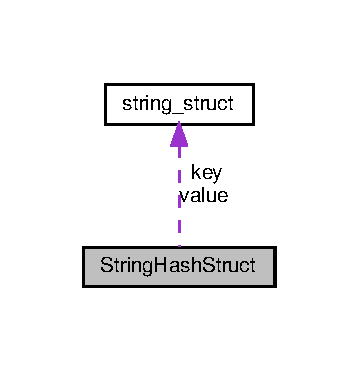
\includegraphics[width=172pt]{struct_string_hash_struct__coll__graph}
\end{center}
\end{figure}
\subsection*{Data Fields}
\begin{DoxyCompactItemize}
\item 
\hyperlink{string_8h_a3d2981d9da3e25dd89371059777fdd12}{string} $\ast$ \hyperlink{struct_string_hash_struct_ad3cf34b56feec46985e00e0854246e15}{key}
\begin{DoxyCompactList}\small\item\em key of hash element \end{DoxyCompactList}\item 
\hyperlink{string_8h_a3d2981d9da3e25dd89371059777fdd12}{string} $\ast$ \hyperlink{struct_string_hash_struct_ad449ecfeb67fd201ad7ece234f18823b}{value}
\begin{DoxyCompactList}\small\item\em corresponding value \end{DoxyCompactList}\end{DoxyCompactItemize}


\subsection{Detailed Description}
Hash element. 

\begin{DoxyAuthor}{Author}
Björn Marx 
\end{DoxyAuthor}


\subsection{Field Documentation}
\mbox{\Hypertarget{struct_string_hash_struct_ad3cf34b56feec46985e00e0854246e15}\label{struct_string_hash_struct_ad3cf34b56feec46985e00e0854246e15}} 
\index{String\+Hash\+Struct@{String\+Hash\+Struct}!key@{key}}
\index{key@{key}!String\+Hash\+Struct@{String\+Hash\+Struct}}
\subsubsection{\texorpdfstring{key}{key}}
{\footnotesize\ttfamily \hyperlink{string_8h_a3d2981d9da3e25dd89371059777fdd12}{string}$\ast$ key}



key of hash element 

\mbox{\Hypertarget{struct_string_hash_struct_ad449ecfeb67fd201ad7ece234f18823b}\label{struct_string_hash_struct_ad449ecfeb67fd201ad7ece234f18823b}} 
\index{String\+Hash\+Struct@{String\+Hash\+Struct}!value@{value}}
\index{value@{value}!String\+Hash\+Struct@{String\+Hash\+Struct}}
\subsubsection{\texorpdfstring{value}{value}}
{\footnotesize\ttfamily \hyperlink{string_8h_a3d2981d9da3e25dd89371059777fdd12}{string}$\ast$ value}



corresponding value 



The documentation for this struct was generated from the following file\+:\begin{DoxyCompactItemize}
\item 
\hyperlink{hash_8h}{hash.\+h}\end{DoxyCompactItemize}

\chapter{File Documentation}
\hypertarget{authorization_8c}{}\section{authorization.\+c File Reference}
\label{authorization_8c}\index{authorization.\+c@{authorization.\+c}}
{\ttfamily \#include \char`\"{}authorization.\+h\char`\"{}}\newline
{\ttfamily \#include \char`\"{}hash.\+h\char`\"{}}\newline
{\ttfamily \#include \char`\"{}base64.\+h\char`\"{}}\newline
{\ttfamily \#include $<$unistd.\+h$>$}\newline
{\ttfamily \#include $<$openssl/sha.\+h$>$}\newline
Include dependency graph for authorization.\+c\+:
\nopagebreak
\begin{figure}[H]
\begin{center}
\leavevmode
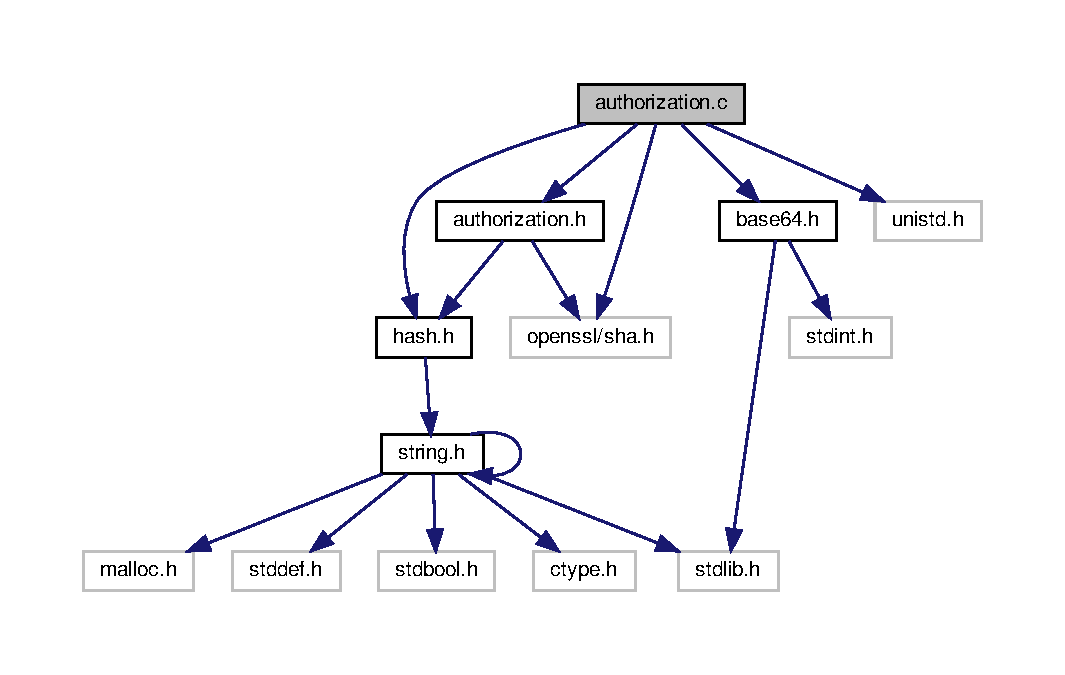
\includegraphics[width=350pt]{authorization_8c__incl}
\end{center}
\end{figure}
\subsection*{Macros}
\begin{DoxyCompactItemize}
\item 
\#define \hyperlink{authorization_8c_a625c76f362da15a712974d925f99229b}{P\+A\+T\+H\+\_\+\+C\+A\+P\+A\+C\+I\+TY}~2083
\item 
\#define \hyperlink{authorization_8c_a3e6fc1fdb6d81b13f26c16eb5efddf19}{P\+A\+T\+H\+\_\+\+C\+A\+P\+A\+C\+I\+T\+Y\+\_\+\+A\+B\+S\+O\+L\+U\+TE}~(\hyperlink{request_8c_a625c76f362da15a712974d925f99229b}{P\+A\+T\+H\+\_\+\+C\+A\+P\+A\+C\+I\+TY} + 200)
\end{DoxyCompactItemize}
\subsection*{Functions}
\begin{DoxyCompactItemize}
\item 
bool \hyperlink{authorization_8c_a854b113e46df11a095cd1291450029a5}{abfrage\+\_\+authorizaition} (\hyperlink{hash_8h_a58bb615f9115c5b9b1a49a64d3737edf}{Hash\+List} $\ast$hashlist)
\item 
\hyperlink{hash_8h_aaae8e320515f4ba6ab5e8bc4ecd7f58a}{Hash} \hyperlink{authorization_8c_a4185038e2e2df6b669ab6250bb891eb8}{password\+\_\+to\+\_\+sha1\+Base64} (\hyperlink{hash_8h_a58bb615f9115c5b9b1a49a64d3737edf}{Hash\+List} $\ast$hashlist)
\item 
bool \hyperlink{authorization_8c_a2d16c0f0b9bd4ad97f067b47455472bf}{authorizaition} (\hyperlink{hash_8h_a58bb615f9115c5b9b1a49a64d3737edf}{Hash\+List} $\ast$hashlist)
\item 
\hyperlink{string_8h_a3d2981d9da3e25dd89371059777fdd12}{string} $\ast$ \hyperlink{authorization_8c_acc2e18e46f4d51886041fc7065adb348}{pw\+\_\+rood} ()
\item 
bool \hyperlink{authorization_8c_aa09030fd3c5bd394c8edc5509330bf23}{read\+\_\+pw\+\_\+list} (\hyperlink{hash_8h_aaae8e320515f4ba6ab5e8bc4ecd7f58a}{Hash} $\ast$hash)
\end{DoxyCompactItemize}


\subsection{Macro Definition Documentation}
\mbox{\Hypertarget{authorization_8c_a625c76f362da15a712974d925f99229b}\label{authorization_8c_a625c76f362da15a712974d925f99229b}} 
\index{authorization.\+c@{authorization.\+c}!P\+A\+T\+H\+\_\+\+C\+A\+P\+A\+C\+I\+TY@{P\+A\+T\+H\+\_\+\+C\+A\+P\+A\+C\+I\+TY}}
\index{P\+A\+T\+H\+\_\+\+C\+A\+P\+A\+C\+I\+TY@{P\+A\+T\+H\+\_\+\+C\+A\+P\+A\+C\+I\+TY}!authorization.\+c@{authorization.\+c}}
\subsubsection{\texorpdfstring{P\+A\+T\+H\+\_\+\+C\+A\+P\+A\+C\+I\+TY}{PATH\_CAPACITY}}
{\footnotesize\ttfamily \#define P\+A\+T\+H\+\_\+\+C\+A\+P\+A\+C\+I\+TY~2083}

\mbox{\Hypertarget{authorization_8c_a3e6fc1fdb6d81b13f26c16eb5efddf19}\label{authorization_8c_a3e6fc1fdb6d81b13f26c16eb5efddf19}} 
\index{authorization.\+c@{authorization.\+c}!P\+A\+T\+H\+\_\+\+C\+A\+P\+A\+C\+I\+T\+Y\+\_\+\+A\+B\+S\+O\+L\+U\+TE@{P\+A\+T\+H\+\_\+\+C\+A\+P\+A\+C\+I\+T\+Y\+\_\+\+A\+B\+S\+O\+L\+U\+TE}}
\index{P\+A\+T\+H\+\_\+\+C\+A\+P\+A\+C\+I\+T\+Y\+\_\+\+A\+B\+S\+O\+L\+U\+TE@{P\+A\+T\+H\+\_\+\+C\+A\+P\+A\+C\+I\+T\+Y\+\_\+\+A\+B\+S\+O\+L\+U\+TE}!authorization.\+c@{authorization.\+c}}
\subsubsection{\texorpdfstring{P\+A\+T\+H\+\_\+\+C\+A\+P\+A\+C\+I\+T\+Y\+\_\+\+A\+B\+S\+O\+L\+U\+TE}{PATH\_CAPACITY\_ABSOLUTE}}
{\footnotesize\ttfamily \#define P\+A\+T\+H\+\_\+\+C\+A\+P\+A\+C\+I\+T\+Y\+\_\+\+A\+B\+S\+O\+L\+U\+TE~(\hyperlink{request_8c_a625c76f362da15a712974d925f99229b}{P\+A\+T\+H\+\_\+\+C\+A\+P\+A\+C\+I\+TY} + 200)}



\subsection{Function Documentation}
\mbox{\Hypertarget{authorization_8c_a854b113e46df11a095cd1291450029a5}\label{authorization_8c_a854b113e46df11a095cd1291450029a5}} 
\index{authorization.\+c@{authorization.\+c}!abfrage\+\_\+authorizaition@{abfrage\+\_\+authorizaition}}
\index{abfrage\+\_\+authorizaition@{abfrage\+\_\+authorizaition}!authorization.\+c@{authorization.\+c}}
\subsubsection{\texorpdfstring{abfrage\+\_\+authorizaition()}{abfrage\_authorizaition()}}
{\footnotesize\ttfamily bool abfrage\+\_\+authorizaition (\begin{DoxyParamCaption}\item[{\hyperlink{hash_8h_a58bb615f9115c5b9b1a49a64d3737edf}{Hash\+List} $\ast$}]{hashlist }\end{DoxyParamCaption})}

Checks whether an authorization header exists \begin{DoxyAuthor}{Author}
Luise 
\end{DoxyAuthor}

\begin{DoxyParams}{Parameters}
{\em hashlist} & Anfrage \\
\hline
\end{DoxyParams}
\begin{DoxyReturn}{Returns}
bool \+: true / false 
\end{DoxyReturn}
\mbox{\Hypertarget{authorization_8c_a2d16c0f0b9bd4ad97f067b47455472bf}\label{authorization_8c_a2d16c0f0b9bd4ad97f067b47455472bf}} 
\index{authorization.\+c@{authorization.\+c}!authorizaition@{authorizaition}}
\index{authorizaition@{authorizaition}!authorization.\+c@{authorization.\+c}}
\subsubsection{\texorpdfstring{authorizaition()}{authorizaition()}}
{\footnotesize\ttfamily bool authorizaition (\begin{DoxyParamCaption}\item[{\hyperlink{hash_8h_a58bb615f9115c5b9b1a49a64d3737edf}{Hash\+List} $\ast$}]{hashlist }\end{DoxyParamCaption})}

Checks whether an authorization header exists and if username and password are correct. \begin{DoxyAuthor}{Author}
Luise 
\end{DoxyAuthor}

\begin{DoxyParams}{Parameters}
{\em hashlist} & \\
\hline
\end{DoxyParams}
\begin{DoxyReturn}{Returns}
bool \+: true / false 
\end{DoxyReturn}
\mbox{\Hypertarget{authorization_8c_a4185038e2e2df6b669ab6250bb891eb8}\label{authorization_8c_a4185038e2e2df6b669ab6250bb891eb8}} 
\index{authorization.\+c@{authorization.\+c}!password\+\_\+to\+\_\+sha1\+Base64@{password\+\_\+to\+\_\+sha1\+Base64}}
\index{password\+\_\+to\+\_\+sha1\+Base64@{password\+\_\+to\+\_\+sha1\+Base64}!authorization.\+c@{authorization.\+c}}
\subsubsection{\texorpdfstring{password\+\_\+to\+\_\+sha1\+Base64()}{password\_to\_sha1Base64()}}
{\footnotesize\ttfamily \hyperlink{hash_8h_aaae8e320515f4ba6ab5e8bc4ecd7f58a}{Hash} password\+\_\+to\+\_\+sha1\+Base64 (\begin{DoxyParamCaption}\item[{\hyperlink{hash_8h_a58bb615f9115c5b9b1a49a64d3737edf}{Hash\+List} $\ast$}]{hashlist }\end{DoxyParamCaption})}

Reads the password and the name from the hashlist and returns a Hash with the Name and the sha1 and Base 64 encoded Password. \begin{DoxyAuthor}{Author}
Jost 
\end{DoxyAuthor}
\begin{DoxyWarning}{Warning}
The returned Hash must be freed 
\end{DoxyWarning}

\begin{DoxyParams}{Parameters}
{\em hashlist} & Hasch\+List with the Name and Password. \\
\hline
\end{DoxyParams}
\begin{DoxyReturn}{Returns}
hash that contains the name(clear text) as the key, and the password (S\+H\+A1 and Base64 encoded) as the value 
\end{DoxyReturn}
\mbox{\Hypertarget{authorization_8c_acc2e18e46f4d51886041fc7065adb348}\label{authorization_8c_acc2e18e46f4d51886041fc7065adb348}} 
\index{authorization.\+c@{authorization.\+c}!pw\+\_\+rood@{pw\+\_\+rood}}
\index{pw\+\_\+rood@{pw\+\_\+rood}!authorization.\+c@{authorization.\+c}}
\subsubsection{\texorpdfstring{pw\+\_\+rood()}{pw\_rood()}}
{\footnotesize\ttfamily \hyperlink{string_8h_a3d2981d9da3e25dd89371059777fdd12}{string}$\ast$ pw\+\_\+rood (\begin{DoxyParamCaption}{ }\end{DoxyParamCaption})}

Created the Password-\/rood-\/string \begin{DoxyAuthor}{Author}
Luise 
\end{DoxyAuthor}
\begin{DoxyWarning}{Warning}
the return string must been freed 
\end{DoxyWarning}
\begin{DoxyReturn}{Returns}
string \+: password\+\_\+rood 
\end{DoxyReturn}
\mbox{\Hypertarget{authorization_8c_aa09030fd3c5bd394c8edc5509330bf23}\label{authorization_8c_aa09030fd3c5bd394c8edc5509330bf23}} 
\index{authorization.\+c@{authorization.\+c}!read\+\_\+pw\+\_\+list@{read\+\_\+pw\+\_\+list}}
\index{read\+\_\+pw\+\_\+list@{read\+\_\+pw\+\_\+list}!authorization.\+c@{authorization.\+c}}
\subsubsection{\texorpdfstring{read\+\_\+pw\+\_\+list()}{read\_pw\_list()}}
{\footnotesize\ttfamily bool read\+\_\+pw\+\_\+list (\begin{DoxyParamCaption}\item[{\hyperlink{hash_8h_aaae8e320515f4ba6ab5e8bc4ecd7f58a}{Hash} $\ast$}]{hash }\end{DoxyParamCaption})}

Checks if username and password are a correct pair. \begin{DoxyAuthor}{Authors}
Jost, Marc 
\end{DoxyAuthor}

\begin{DoxyParams}{Parameters}
{\em hash} & that contains the name(clear text) as the key, and the password (S\+H\+A1 encoded) as the value \\
\hline
\end{DoxyParams}
\begin{DoxyReturn}{Returns}
bool is true if the password and name match the htpasswd file 
\end{DoxyReturn}

\hypertarget{authorization_8h}{}\section{authorization.\+h File Reference}
\label{authorization_8h}\index{authorization.\+h@{authorization.\+h}}
{\ttfamily \#include \char`\"{}hash.\+h\char`\"{}}\newline
{\ttfamily \#include $<$openssl/sha.\+h$>$}\newline
Include dependency graph for authorization.\+h\+:
\nopagebreak
\begin{figure}[H]
\begin{center}
\leavevmode
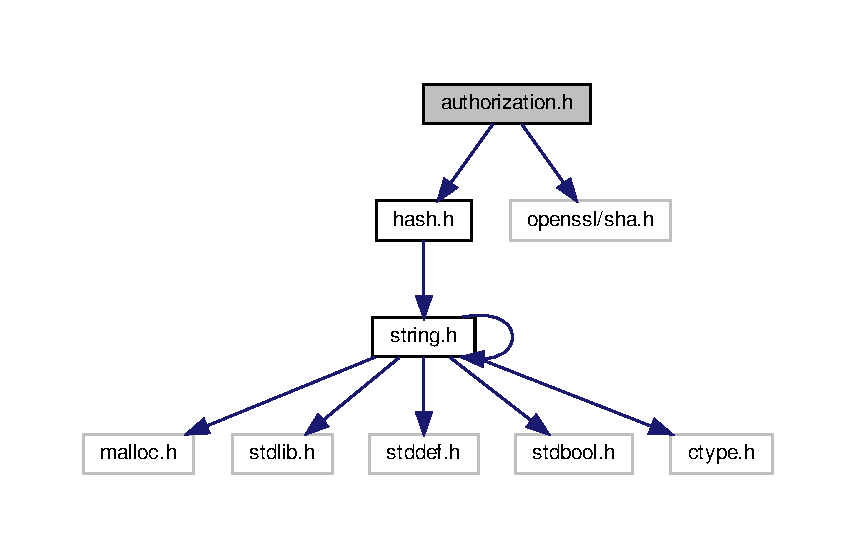
\includegraphics[width=350pt]{authorization_8h__incl}
\end{center}
\end{figure}
This graph shows which files directly or indirectly include this file\+:
\nopagebreak
\begin{figure}[H]
\begin{center}
\leavevmode
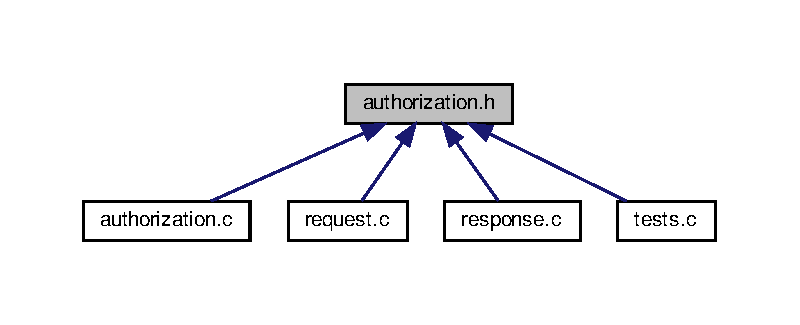
\includegraphics[width=350pt]{authorization_8h__dep__incl}
\end{center}
\end{figure}
\subsection*{Macros}
\begin{DoxyCompactItemize}
\item 
\#define \hyperlink{authorization_8h_adb206c2b1e09e3b45275c256b8686488}{P\+S\+E20\+\_\+\+A\+U\+T\+H\+O\+R\+I\+Z\+A\+T\+I\+O\+N\+\_\+H}
\end{DoxyCompactItemize}
\subsection*{Functions}
\begin{DoxyCompactItemize}
\item 
bool \hyperlink{authorization_8h_a854b113e46df11a095cd1291450029a5}{abfrage\+\_\+authorizaition} (\hyperlink{hash_8h_a58bb615f9115c5b9b1a49a64d3737edf}{Hash\+List} $\ast$hashlist)
\item 
bool \hyperlink{authorization_8h_ac3929cbc3c23632557e2caad136a806a}{passwort\+\_\+abfrage\+\_\+authorizaition} (\hyperlink{hash_8h_a58bb615f9115c5b9b1a49a64d3737edf}{Hash\+List} $\ast$hashlist)
\item 
\hyperlink{hash_8h_aaae8e320515f4ba6ab5e8bc4ecd7f58a}{Hash} \hyperlink{authorization_8h_a4185038e2e2df6b669ab6250bb891eb8}{password\+\_\+to\+\_\+sha1\+Base64} (\hyperlink{hash_8h_a58bb615f9115c5b9b1a49a64d3737edf}{Hash\+List} $\ast$hashlist)
\item 
bool \hyperlink{authorization_8h_aa09030fd3c5bd394c8edc5509330bf23}{read\+\_\+pw\+\_\+list} (\hyperlink{hash_8h_aaae8e320515f4ba6ab5e8bc4ecd7f58a}{Hash} $\ast$hash)
\item 
\hyperlink{string_8h_a3d2981d9da3e25dd89371059777fdd12}{string} $\ast$ \hyperlink{authorization_8h_acc2e18e46f4d51886041fc7065adb348}{pw\+\_\+rood} ()
\item 
bool \hyperlink{authorization_8h_a2d16c0f0b9bd4ad97f067b47455472bf}{authorizaition} (\hyperlink{hash_8h_a58bb615f9115c5b9b1a49a64d3737edf}{Hash\+List} $\ast$hashlist)
\end{DoxyCompactItemize}


\subsection{Detailed Description}
\begin{DoxyAuthor}{Author}
P\+SE 17 
\end{DoxyAuthor}


\subsection{Macro Definition Documentation}
\mbox{\Hypertarget{authorization_8h_adb206c2b1e09e3b45275c256b8686488}\label{authorization_8h_adb206c2b1e09e3b45275c256b8686488}} 
\index{authorization.\+h@{authorization.\+h}!P\+S\+E20\+\_\+\+A\+U\+T\+H\+O\+R\+I\+Z\+A\+T\+I\+O\+N\+\_\+H@{P\+S\+E20\+\_\+\+A\+U\+T\+H\+O\+R\+I\+Z\+A\+T\+I\+O\+N\+\_\+H}}
\index{P\+S\+E20\+\_\+\+A\+U\+T\+H\+O\+R\+I\+Z\+A\+T\+I\+O\+N\+\_\+H@{P\+S\+E20\+\_\+\+A\+U\+T\+H\+O\+R\+I\+Z\+A\+T\+I\+O\+N\+\_\+H}!authorization.\+h@{authorization.\+h}}
\subsubsection{\texorpdfstring{P\+S\+E20\+\_\+\+A\+U\+T\+H\+O\+R\+I\+Z\+A\+T\+I\+O\+N\+\_\+H}{PSE20\_AUTHORIZATION\_H}}
{\footnotesize\ttfamily \#define P\+S\+E20\+\_\+\+A\+U\+T\+H\+O\+R\+I\+Z\+A\+T\+I\+O\+N\+\_\+H}



\subsection{Function Documentation}
\mbox{\Hypertarget{authorization_8h_a854b113e46df11a095cd1291450029a5}\label{authorization_8h_a854b113e46df11a095cd1291450029a5}} 
\index{authorization.\+h@{authorization.\+h}!abfrage\+\_\+authorizaition@{abfrage\+\_\+authorizaition}}
\index{abfrage\+\_\+authorizaition@{abfrage\+\_\+authorizaition}!authorization.\+h@{authorization.\+h}}
\subsubsection{\texorpdfstring{abfrage\+\_\+authorizaition()}{abfrage\_authorizaition()}}
{\footnotesize\ttfamily bool abfrage\+\_\+authorizaition (\begin{DoxyParamCaption}\item[{\hyperlink{hash_8h_a58bb615f9115c5b9b1a49a64d3737edf}{Hash\+List} $\ast$}]{hashlist }\end{DoxyParamCaption})}

Checks whether an authorization header exists \begin{DoxyAuthor}{Author}
Luise 
\end{DoxyAuthor}

\begin{DoxyParams}{Parameters}
{\em hashlist} & Anfrage \\
\hline
\end{DoxyParams}
\begin{DoxyReturn}{Returns}
bool \+: true / false 
\end{DoxyReturn}
\mbox{\Hypertarget{authorization_8h_a2d16c0f0b9bd4ad97f067b47455472bf}\label{authorization_8h_a2d16c0f0b9bd4ad97f067b47455472bf}} 
\index{authorization.\+h@{authorization.\+h}!authorizaition@{authorizaition}}
\index{authorizaition@{authorizaition}!authorization.\+h@{authorization.\+h}}
\subsubsection{\texorpdfstring{authorizaition()}{authorizaition()}}
{\footnotesize\ttfamily bool authorizaition (\begin{DoxyParamCaption}\item[{\hyperlink{hash_8h_a58bb615f9115c5b9b1a49a64d3737edf}{Hash\+List} $\ast$}]{hashlist }\end{DoxyParamCaption})}

Checks whether an authorization header exists and if username and password are correct. \begin{DoxyAuthor}{Author}
Luise 
\end{DoxyAuthor}

\begin{DoxyParams}{Parameters}
{\em hashlist} & \\
\hline
\end{DoxyParams}
\begin{DoxyReturn}{Returns}
bool \+: true / false 
\end{DoxyReturn}
\mbox{\Hypertarget{authorization_8h_a4185038e2e2df6b669ab6250bb891eb8}\label{authorization_8h_a4185038e2e2df6b669ab6250bb891eb8}} 
\index{authorization.\+h@{authorization.\+h}!password\+\_\+to\+\_\+sha1\+Base64@{password\+\_\+to\+\_\+sha1\+Base64}}
\index{password\+\_\+to\+\_\+sha1\+Base64@{password\+\_\+to\+\_\+sha1\+Base64}!authorization.\+h@{authorization.\+h}}
\subsubsection{\texorpdfstring{password\+\_\+to\+\_\+sha1\+Base64()}{password\_to\_sha1Base64()}}
{\footnotesize\ttfamily \hyperlink{hash_8h_aaae8e320515f4ba6ab5e8bc4ecd7f58a}{Hash} password\+\_\+to\+\_\+sha1\+Base64 (\begin{DoxyParamCaption}\item[{\hyperlink{hash_8h_a58bb615f9115c5b9b1a49a64d3737edf}{Hash\+List} $\ast$}]{hashlist }\end{DoxyParamCaption})}

Reads the password and the name from the hashlist and returns a Hash with the Name and the sha1 and Base 64 encoded Password. \begin{DoxyAuthor}{Author}
Jost 
\end{DoxyAuthor}
\begin{DoxyWarning}{Warning}
The returned Hash must be freed 
\end{DoxyWarning}

\begin{DoxyParams}{Parameters}
{\em hashlist} & Hasch\+List with the Name and Password. \\
\hline
\end{DoxyParams}
\begin{DoxyReturn}{Returns}
hash that contains the name(clear text) as the key, and the password (S\+H\+A1 and Base64 encoded) as the value 
\end{DoxyReturn}
\mbox{\Hypertarget{authorization_8h_ac3929cbc3c23632557e2caad136a806a}\label{authorization_8h_ac3929cbc3c23632557e2caad136a806a}} 
\index{authorization.\+h@{authorization.\+h}!passwort\+\_\+abfrage\+\_\+authorizaition@{passwort\+\_\+abfrage\+\_\+authorizaition}}
\index{passwort\+\_\+abfrage\+\_\+authorizaition@{passwort\+\_\+abfrage\+\_\+authorizaition}!authorization.\+h@{authorization.\+h}}
\subsubsection{\texorpdfstring{passwort\+\_\+abfrage\+\_\+authorizaition()}{passwort\_abfrage\_authorizaition()}}
{\footnotesize\ttfamily bool passwort\+\_\+abfrage\+\_\+authorizaition (\begin{DoxyParamCaption}\item[{\hyperlink{hash_8h_a58bb615f9115c5b9b1a49a64d3737edf}{Hash\+List} $\ast$}]{hashlist }\end{DoxyParamCaption})}

verschlüsselung das Passworts 
\begin{DoxyParams}{Parameters}
{\em hashlist} & \\
\hline
\end{DoxyParams}
\begin{DoxyReturn}{Returns}

\end{DoxyReturn}
\mbox{\Hypertarget{authorization_8h_acc2e18e46f4d51886041fc7065adb348}\label{authorization_8h_acc2e18e46f4d51886041fc7065adb348}} 
\index{authorization.\+h@{authorization.\+h}!pw\+\_\+rood@{pw\+\_\+rood}}
\index{pw\+\_\+rood@{pw\+\_\+rood}!authorization.\+h@{authorization.\+h}}
\subsubsection{\texorpdfstring{pw\+\_\+rood()}{pw\_rood()}}
{\footnotesize\ttfamily \hyperlink{string_8h_a3d2981d9da3e25dd89371059777fdd12}{string}$\ast$ pw\+\_\+rood (\begin{DoxyParamCaption}{ }\end{DoxyParamCaption})}

Created the Password-\/rood-\/string \begin{DoxyAuthor}{Author}
Luise 
\end{DoxyAuthor}
\begin{DoxyWarning}{Warning}
the return string must been freed 
\end{DoxyWarning}
\begin{DoxyReturn}{Returns}
string \+: password\+\_\+rood 
\end{DoxyReturn}
\mbox{\Hypertarget{authorization_8h_aa09030fd3c5bd394c8edc5509330bf23}\label{authorization_8h_aa09030fd3c5bd394c8edc5509330bf23}} 
\index{authorization.\+h@{authorization.\+h}!read\+\_\+pw\+\_\+list@{read\+\_\+pw\+\_\+list}}
\index{read\+\_\+pw\+\_\+list@{read\+\_\+pw\+\_\+list}!authorization.\+h@{authorization.\+h}}
\subsubsection{\texorpdfstring{read\+\_\+pw\+\_\+list()}{read\_pw\_list()}}
{\footnotesize\ttfamily bool read\+\_\+pw\+\_\+list (\begin{DoxyParamCaption}\item[{\hyperlink{hash_8h_aaae8e320515f4ba6ab5e8bc4ecd7f58a}{Hash} $\ast$}]{hash }\end{DoxyParamCaption})}

Checks if username and password are a correct pair. \begin{DoxyAuthor}{Authors}
Jost, Marc 
\end{DoxyAuthor}

\begin{DoxyParams}{Parameters}
{\em hash} & that contains the name(clear text) as the key, and the password (S\+H\+A1 encoded) as the value \\
\hline
\end{DoxyParams}
\begin{DoxyReturn}{Returns}
bool is true if the password and name match the htpasswd file 
\end{DoxyReturn}

\hypertarget{base64_8c}{}\section{base64.\+c File Reference}
\label{base64_8c}\index{base64.\+c@{base64.\+c}}
{\ttfamily \#include \char`\"{}base64.\+h\char`\"{}}\newline
{\ttfamily \#include $<$stdint.\+h$>$}\newline
{\ttfamily \#include $<$stdlib.\+h$>$}\newline
Include dependency graph for base64.\+c\+:
\nopagebreak
\begin{figure}[H]
\begin{center}
\leavevmode
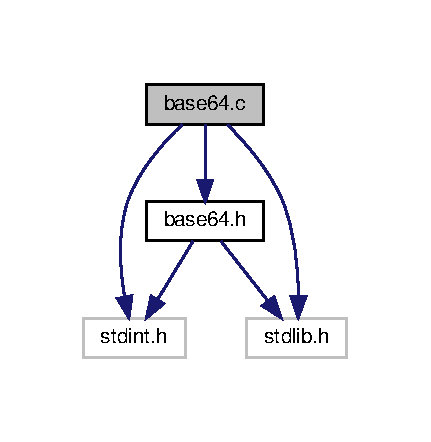
\includegraphics[width=207pt]{base64_8c__incl}
\end{center}
\end{figure}
\subsection*{Functions}
\begin{DoxyCompactItemize}
\item 
void \hyperlink{base64_8c_afc1c382e496a1949a4bf13fe1cadbea7}{build\+\_\+decoding\+\_\+table1} ()
\item 
char $\ast$ \hyperlink{base64_8c_aab78ff2ac8c7390cd6755ce3a55eaa21}{base64\+\_\+encode} (const unsigned char $\ast$data, size\+\_\+t input\+\_\+length, size\+\_\+t $\ast$output\+\_\+length)
\item 
unsigned char $\ast$ \hyperlink{base64_8c_a093de76493e254154a5ccee90672244b}{base64\+\_\+decode} (const char $\ast$data, size\+\_\+t input\+\_\+length, size\+\_\+t $\ast$output\+\_\+length)
\item 
void \hyperlink{base64_8c_a24c1b02f2e403468ce12faa8374877c1}{base64\+\_\+cleanup} ()
\end{DoxyCompactItemize}


\subsection{Function Documentation}
\mbox{\Hypertarget{base64_8c_a24c1b02f2e403468ce12faa8374877c1}\label{base64_8c_a24c1b02f2e403468ce12faa8374877c1}} 
\index{base64.\+c@{base64.\+c}!base64\+\_\+cleanup@{base64\+\_\+cleanup}}
\index{base64\+\_\+cleanup@{base64\+\_\+cleanup}!base64.\+c@{base64.\+c}}
\subsubsection{\texorpdfstring{base64\+\_\+cleanup()}{base64\_cleanup()}}
{\footnotesize\ttfamily void base64\+\_\+cleanup (\begin{DoxyParamCaption}{ }\end{DoxyParamCaption})}

\mbox{\Hypertarget{base64_8c_a093de76493e254154a5ccee90672244b}\label{base64_8c_a093de76493e254154a5ccee90672244b}} 
\index{base64.\+c@{base64.\+c}!base64\+\_\+decode@{base64\+\_\+decode}}
\index{base64\+\_\+decode@{base64\+\_\+decode}!base64.\+c@{base64.\+c}}
\subsubsection{\texorpdfstring{base64\+\_\+decode()}{base64\_decode()}}
{\footnotesize\ttfamily unsigned char$\ast$ base64\+\_\+decode (\begin{DoxyParamCaption}\item[{const char $\ast$}]{data,  }\item[{size\+\_\+t}]{input\+\_\+length,  }\item[{size\+\_\+t $\ast$}]{output\+\_\+length }\end{DoxyParamCaption})}

\mbox{\Hypertarget{base64_8c_aab78ff2ac8c7390cd6755ce3a55eaa21}\label{base64_8c_aab78ff2ac8c7390cd6755ce3a55eaa21}} 
\index{base64.\+c@{base64.\+c}!base64\+\_\+encode@{base64\+\_\+encode}}
\index{base64\+\_\+encode@{base64\+\_\+encode}!base64.\+c@{base64.\+c}}
\subsubsection{\texorpdfstring{base64\+\_\+encode()}{base64\_encode()}}
{\footnotesize\ttfamily char$\ast$ base64\+\_\+encode (\begin{DoxyParamCaption}\item[{const unsigned char $\ast$}]{data,  }\item[{size\+\_\+t}]{input\+\_\+length,  }\item[{size\+\_\+t $\ast$}]{output\+\_\+length }\end{DoxyParamCaption})}

\mbox{\Hypertarget{base64_8c_afc1c382e496a1949a4bf13fe1cadbea7}\label{base64_8c_afc1c382e496a1949a4bf13fe1cadbea7}} 
\index{base64.\+c@{base64.\+c}!build\+\_\+decoding\+\_\+table1@{build\+\_\+decoding\+\_\+table1}}
\index{build\+\_\+decoding\+\_\+table1@{build\+\_\+decoding\+\_\+table1}!base64.\+c@{base64.\+c}}
\subsubsection{\texorpdfstring{build\+\_\+decoding\+\_\+table1()}{build\_decoding\_table1()}}
{\footnotesize\ttfamily void build\+\_\+decoding\+\_\+table1 (\begin{DoxyParamCaption}{ }\end{DoxyParamCaption})}


\hypertarget{base64_8h}{}\section{base64.\+h File Reference}
\label{base64_8h}\index{base64.\+h@{base64.\+h}}
{\ttfamily \#include $<$stdint.\+h$>$}\newline
{\ttfamily \#include $<$stdlib.\+h$>$}\newline
Include dependency graph for base64.\+h\+:
\nopagebreak
\begin{figure}[H]
\begin{center}
\leavevmode
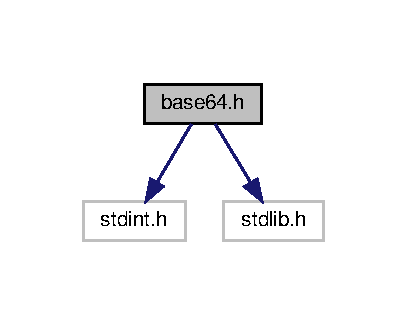
\includegraphics[width=196pt]{base64_8h__incl}
\end{center}
\end{figure}
This graph shows which files directly or indirectly include this file\+:
\nopagebreak
\begin{figure}[H]
\begin{center}
\leavevmode
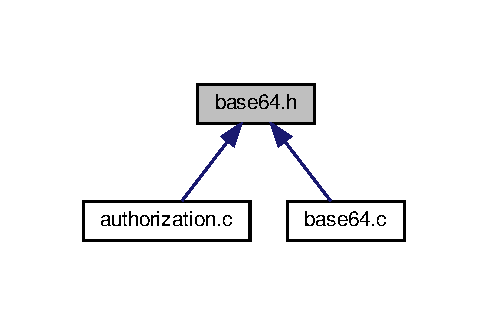
\includegraphics[width=234pt]{base64_8h__dep__incl}
\end{center}
\end{figure}
\subsection*{Functions}
\begin{DoxyCompactItemize}
\item 
void \hyperlink{base64_8h_afc1c382e496a1949a4bf13fe1cadbea7}{build\+\_\+decoding\+\_\+table1} ()
\item 
char $\ast$ \hyperlink{base64_8h_aab78ff2ac8c7390cd6755ce3a55eaa21}{base64\+\_\+encode} (const unsigned char $\ast$data, size\+\_\+t input\+\_\+length, size\+\_\+t $\ast$output\+\_\+length)
\item 
unsigned char $\ast$ \hyperlink{base64_8h_a093de76493e254154a5ccee90672244b}{base64\+\_\+decode} (const char $\ast$data, size\+\_\+t input\+\_\+length, size\+\_\+t $\ast$output\+\_\+length)
\item 
void \hyperlink{base64_8h_a24c1b02f2e403468ce12faa8374877c1}{base64\+\_\+cleanup} ()
\end{DoxyCompactItemize}


\subsection{Function Documentation}
\mbox{\Hypertarget{base64_8h_a24c1b02f2e403468ce12faa8374877c1}\label{base64_8h_a24c1b02f2e403468ce12faa8374877c1}} 
\index{base64.\+h@{base64.\+h}!base64\+\_\+cleanup@{base64\+\_\+cleanup}}
\index{base64\+\_\+cleanup@{base64\+\_\+cleanup}!base64.\+h@{base64.\+h}}
\subsubsection{\texorpdfstring{base64\+\_\+cleanup()}{base64\_cleanup()}}
{\footnotesize\ttfamily void base64\+\_\+cleanup (\begin{DoxyParamCaption}{ }\end{DoxyParamCaption})}

\mbox{\Hypertarget{base64_8h_a093de76493e254154a5ccee90672244b}\label{base64_8h_a093de76493e254154a5ccee90672244b}} 
\index{base64.\+h@{base64.\+h}!base64\+\_\+decode@{base64\+\_\+decode}}
\index{base64\+\_\+decode@{base64\+\_\+decode}!base64.\+h@{base64.\+h}}
\subsubsection{\texorpdfstring{base64\+\_\+decode()}{base64\_decode()}}
{\footnotesize\ttfamily unsigned char$\ast$ base64\+\_\+decode (\begin{DoxyParamCaption}\item[{const char $\ast$}]{data,  }\item[{size\+\_\+t}]{input\+\_\+length,  }\item[{size\+\_\+t $\ast$}]{output\+\_\+length }\end{DoxyParamCaption})}

\mbox{\Hypertarget{base64_8h_aab78ff2ac8c7390cd6755ce3a55eaa21}\label{base64_8h_aab78ff2ac8c7390cd6755ce3a55eaa21}} 
\index{base64.\+h@{base64.\+h}!base64\+\_\+encode@{base64\+\_\+encode}}
\index{base64\+\_\+encode@{base64\+\_\+encode}!base64.\+h@{base64.\+h}}
\subsubsection{\texorpdfstring{base64\+\_\+encode()}{base64\_encode()}}
{\footnotesize\ttfamily char$\ast$ base64\+\_\+encode (\begin{DoxyParamCaption}\item[{const unsigned char $\ast$}]{data,  }\item[{size\+\_\+t}]{input\+\_\+length,  }\item[{size\+\_\+t $\ast$}]{output\+\_\+length }\end{DoxyParamCaption})}

\mbox{\Hypertarget{base64_8h_afc1c382e496a1949a4bf13fe1cadbea7}\label{base64_8h_afc1c382e496a1949a4bf13fe1cadbea7}} 
\index{base64.\+h@{base64.\+h}!build\+\_\+decoding\+\_\+table1@{build\+\_\+decoding\+\_\+table1}}
\index{build\+\_\+decoding\+\_\+table1@{build\+\_\+decoding\+\_\+table1}!base64.\+h@{base64.\+h}}
\subsubsection{\texorpdfstring{build\+\_\+decoding\+\_\+table1()}{build\_decoding\_table1()}}
{\footnotesize\ttfamily void build\+\_\+decoding\+\_\+table1 (\begin{DoxyParamCaption}{ }\end{DoxyParamCaption})}


\hypertarget{echo__server_8c}{}\section{echo\+\_\+server.\+c File Reference}
\label{echo__server_8c}\index{echo\+\_\+server.\+c@{echo\+\_\+server.\+c}}
{\ttfamily \#include $<$errno.\+h$>$}\newline
{\ttfamily \#include $<$netinet/ip.\+h$>$}\newline
{\ttfamily \#include $<$signal.\+h$>$}\newline
{\ttfamily \#include $<$stdbool.\+h$>$}\newline
{\ttfamily \#include $<$stdio.\+h$>$}\newline
{\ttfamily \#include $<$stdlib.\+h$>$}\newline
{\ttfamily \#include $<$string.\+h$>$}\newline
{\ttfamily \#include $<$sys/socket.\+h$>$}\newline
{\ttfamily \#include $<$unistd.\+h$>$}\newline
{\ttfamily \#include $<$poll.\+h$>$}\newline
{\ttfamily \#include $<$openssl/sha.\+h$>$}\newline
{\ttfamily \#include \char`\"{}request.\+h\char`\"{}}\newline
{\ttfamily \#include \char`\"{}response.\+h\char`\"{}}\newline
{\ttfamily \#include \char`\"{}tests.\+h\char`\"{}}\newline
Include dependency graph for echo\+\_\+server.\+c\+:
\nopagebreak
\begin{figure}[H]
\begin{center}
\leavevmode
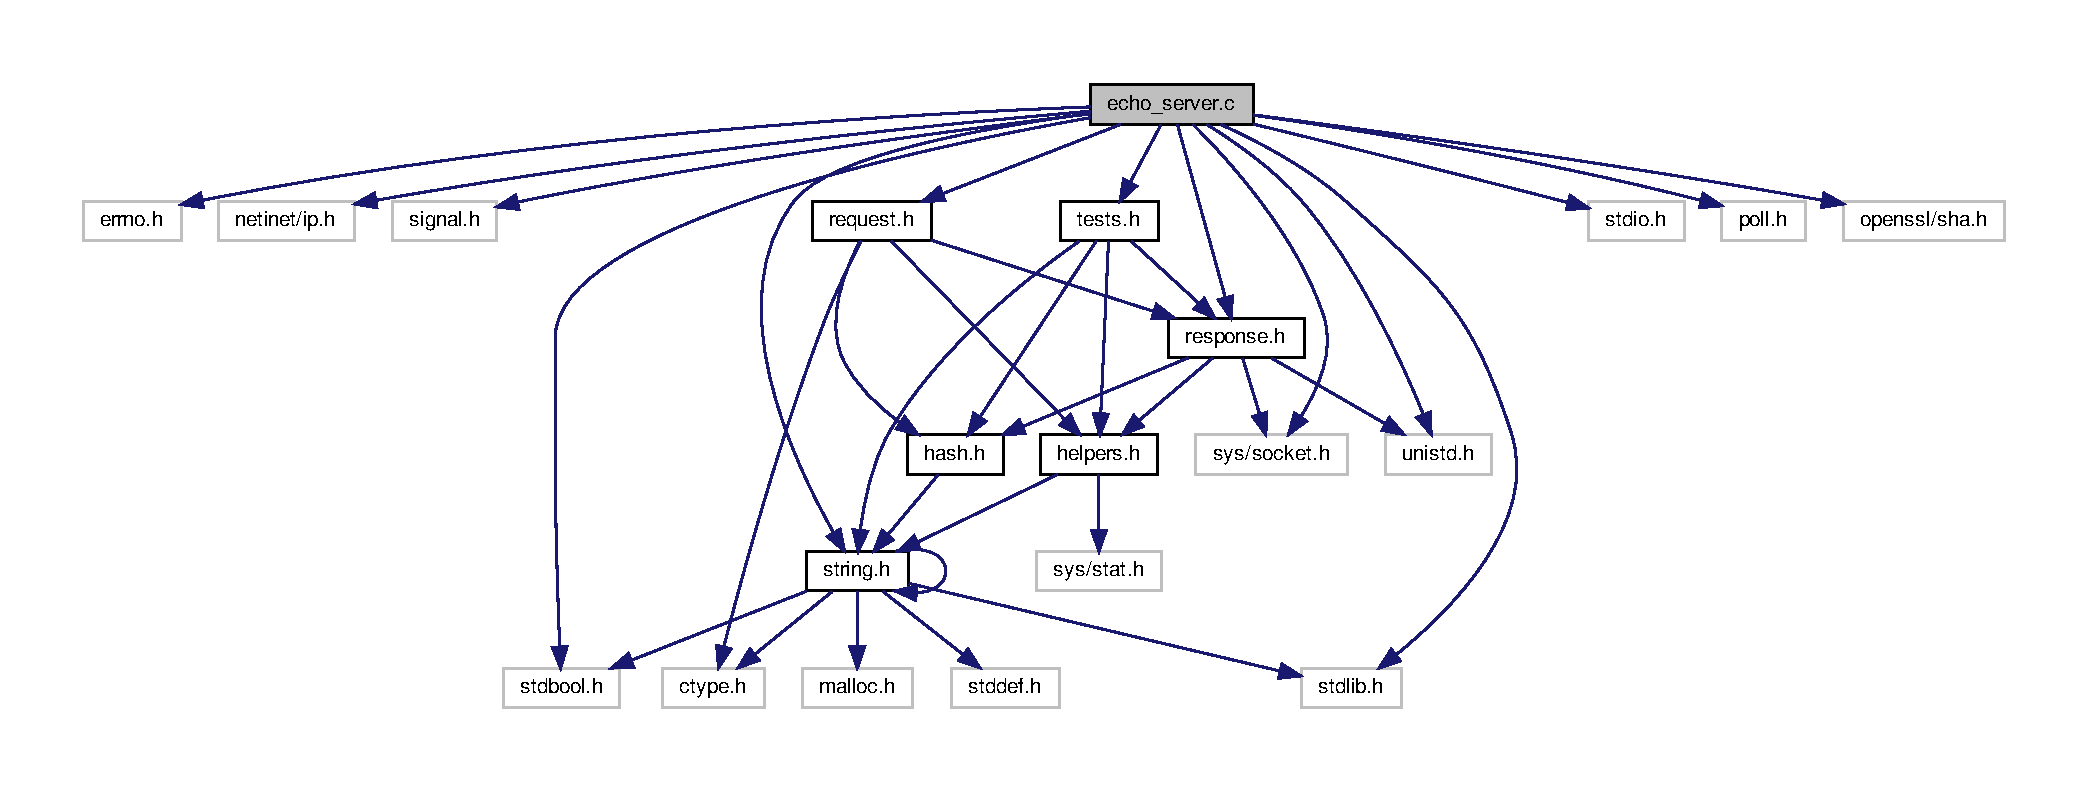
\includegraphics[width=350pt]{echo__server_8c__incl}
\end{center}
\end{figure}
\subsection*{Macros}
\begin{DoxyCompactItemize}
\item 
\#define \hyperlink{echo__server_8c_a614217d263be1fb1a5f76e2ff7be19a2}{P\+O\+RT}~31337
\item 
\#define \hyperlink{echo__server_8c_a6b20d41d6252e9871430c242cb1a56e7}{B\+U\+F\+F\+E\+R\+\_\+\+S\+I\+ZE}~1024
\item 
\#define \hyperlink{echo__server_8c_a76e334e12a376a91d58c9ec5ae9a7abf}{M\+A\+X\+\_\+\+H\+E\+A\+D\+E\+R\+\_\+\+L\+EN}~8192
\end{DoxyCompactItemize}
\subsection*{Functions}
\begin{DoxyCompactItemize}
\item 
int \hyperlink{echo__server_8c_a0ddf1224851353fc92bfbff6f499fa97}{main} (int argc, char $\ast$argv\mbox{[}$\,$\mbox{]})
\end{DoxyCompactItemize}


\subsection{Macro Definition Documentation}
\mbox{\Hypertarget{echo__server_8c_a6b20d41d6252e9871430c242cb1a56e7}\label{echo__server_8c_a6b20d41d6252e9871430c242cb1a56e7}} 
\index{echo\+\_\+server.\+c@{echo\+\_\+server.\+c}!B\+U\+F\+F\+E\+R\+\_\+\+S\+I\+ZE@{B\+U\+F\+F\+E\+R\+\_\+\+S\+I\+ZE}}
\index{B\+U\+F\+F\+E\+R\+\_\+\+S\+I\+ZE@{B\+U\+F\+F\+E\+R\+\_\+\+S\+I\+ZE}!echo\+\_\+server.\+c@{echo\+\_\+server.\+c}}
\subsubsection{\texorpdfstring{B\+U\+F\+F\+E\+R\+\_\+\+S\+I\+ZE}{BUFFER\_SIZE}}
{\footnotesize\ttfamily \#define B\+U\+F\+F\+E\+R\+\_\+\+S\+I\+ZE~1024}

\mbox{\Hypertarget{echo__server_8c_a76e334e12a376a91d58c9ec5ae9a7abf}\label{echo__server_8c_a76e334e12a376a91d58c9ec5ae9a7abf}} 
\index{echo\+\_\+server.\+c@{echo\+\_\+server.\+c}!M\+A\+X\+\_\+\+H\+E\+A\+D\+E\+R\+\_\+\+L\+EN@{M\+A\+X\+\_\+\+H\+E\+A\+D\+E\+R\+\_\+\+L\+EN}}
\index{M\+A\+X\+\_\+\+H\+E\+A\+D\+E\+R\+\_\+\+L\+EN@{M\+A\+X\+\_\+\+H\+E\+A\+D\+E\+R\+\_\+\+L\+EN}!echo\+\_\+server.\+c@{echo\+\_\+server.\+c}}
\subsubsection{\texorpdfstring{M\+A\+X\+\_\+\+H\+E\+A\+D\+E\+R\+\_\+\+L\+EN}{MAX\_HEADER\_LEN}}
{\footnotesize\ttfamily \#define M\+A\+X\+\_\+\+H\+E\+A\+D\+E\+R\+\_\+\+L\+EN~8192}

\mbox{\Hypertarget{echo__server_8c_a614217d263be1fb1a5f76e2ff7be19a2}\label{echo__server_8c_a614217d263be1fb1a5f76e2ff7be19a2}} 
\index{echo\+\_\+server.\+c@{echo\+\_\+server.\+c}!P\+O\+RT@{P\+O\+RT}}
\index{P\+O\+RT@{P\+O\+RT}!echo\+\_\+server.\+c@{echo\+\_\+server.\+c}}
\subsubsection{\texorpdfstring{P\+O\+RT}{PORT}}
{\footnotesize\ttfamily \#define P\+O\+RT~31337}



\subsection{Function Documentation}
\mbox{\Hypertarget{echo__server_8c_a0ddf1224851353fc92bfbff6f499fa97}\label{echo__server_8c_a0ddf1224851353fc92bfbff6f499fa97}} 
\index{echo\+\_\+server.\+c@{echo\+\_\+server.\+c}!main@{main}}
\index{main@{main}!echo\+\_\+server.\+c@{echo\+\_\+server.\+c}}
\subsubsection{\texorpdfstring{main()}{main()}}
{\footnotesize\ttfamily int main (\begin{DoxyParamCaption}\item[{int}]{argc,  }\item[{char $\ast$}]{argv\mbox{[}$\,$\mbox{]} }\end{DoxyParamCaption})}


\hypertarget{hash_8c}{}\section{hash.\+c File Reference}
\label{hash_8c}\index{hash.\+c@{hash.\+c}}
{\ttfamily \#include \char`\"{}hash.\+h\char`\"{}}\newline
Include dependency graph for hash.\+c\+:
\nopagebreak
\begin{figure}[H]
\begin{center}
\leavevmode
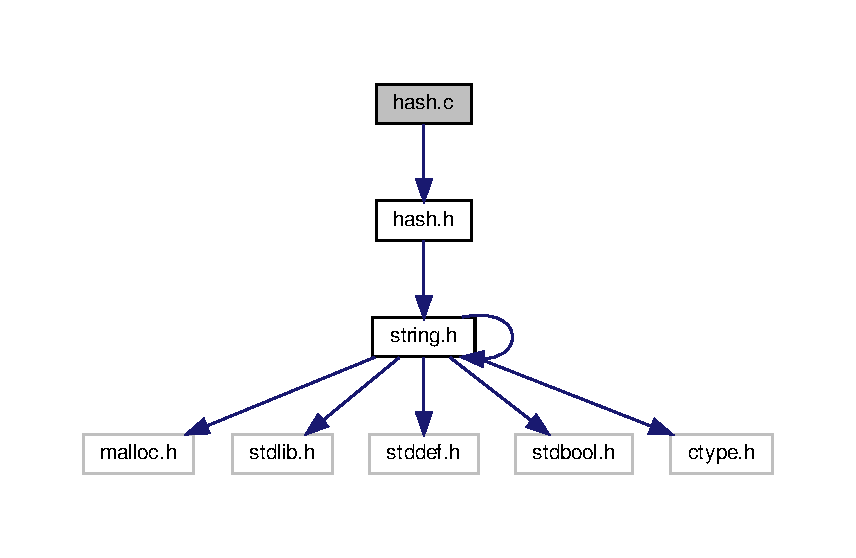
\includegraphics[width=350pt]{hash_8c__incl}
\end{center}
\end{figure}
\subsection*{Functions}
\begin{DoxyCompactItemize}
\item 
\hyperlink{hash_8h_a58bb615f9115c5b9b1a49a64d3737edf}{Hash\+List} $\ast$ \hyperlink{hash_8c_a73d7429aa205aee8b6e38808a8e2f53d}{S\+H\+L\+\_\+create} (\hyperlink{hash_8h_aaae8e320515f4ba6ab5e8bc4ecd7f58a}{Hash} first\+Element)
\begin{DoxyCompactList}\small\item\em creates new list Creates new list, but requires \end{DoxyCompactList}\item 
void \hyperlink{hash_8c_a5bf8ba8e50fdaedb05f2112695ec273c}{S\+H\+L\+\_\+append} (\hyperlink{hash_8h_a58bb615f9115c5b9b1a49a64d3737edf}{Hash\+List} $\ast$first, \hyperlink{hash_8h_aaae8e320515f4ba6ab5e8bc4ecd7f58a}{Hash} next)
\begin{DoxyCompactList}\small\item\em appends a new element at the end \end{DoxyCompactList}\item 
void \hyperlink{hash_8c_a7d3fe6343ca665e7014267c8f4905a9a}{S\+H\+L\+\_\+free\+\_\+element} (\hyperlink{hash_8h_a58bb615f9115c5b9b1a49a64d3737edf}{Hash\+List} $\ast$item)
\begin{DoxyCompactList}\small\item\em frees an element in the the list including it\textquotesingle{}s data\textquotesingle{}s Strings bear in mind that this will N\+OT touch the $\ast$next element \end{DoxyCompactList}\item 
void \hyperlink{hash_8c_a18f61bc4858ec37fc8f1198011c6b4e1}{S\+H\+L\+\_\+remove\+\_\+all} (\hyperlink{hash_8h_a58bb615f9115c5b9b1a49a64d3737edf}{Hash\+List} $\ast$first)
\begin{DoxyCompactList}\small\item\em removes element at position \end{DoxyCompactList}\item 
\hyperlink{hash_8h_aaae8e320515f4ba6ab5e8bc4ecd7f58a}{Hash} $\ast$ \hyperlink{hash_8c_a64a6c39375656b38732e8c3c20d2d9a0}{S\+H\+L\+\_\+find\+\_\+key} (\hyperlink{hash_8h_a58bb615f9115c5b9b1a49a64d3737edf}{Hash\+List} $\ast$first, \hyperlink{string_8h_a3d2981d9da3e25dd89371059777fdd12}{string} $\ast$key)
\begin{DoxyCompactList}\small\item\em returns pointer to the {\itshape F\+I\+R\+ST} element containing key Returns pointer to the {\itshape F\+I\+R\+ST} element containing key, will return N\+U\+LL if key is not found \end{DoxyCompactList}\item 
\hyperlink{hash_8h_aaae8e320515f4ba6ab5e8bc4ecd7f58a}{Hash} \hyperlink{hash_8c_ad0e07fdde374ab0435606a45dcdd58bc}{S\+H\+L\+\_\+at} (\hyperlink{hash_8h_a58bb615f9115c5b9b1a49a64d3737edf}{Hash\+List} $\ast$first, unsigned int index)
\begin{DoxyCompactList}\small\item\em return index\textquotesingle{}th element of Hash\+List function returning the index\textquotesingle{}th element of Hash\+List first, it will return the last element if index is out of bound \end{DoxyCompactList}\item 
\hyperlink{hash_8h_aaae8e320515f4ba6ab5e8bc4ecd7f58a}{Hash} \hyperlink{hash_8c_af3a6014f24a682c18b619d581dd23db4}{S\+H\+\_\+create} (\hyperlink{string_8h_a3d2981d9da3e25dd89371059777fdd12}{string} $\ast$key, \hyperlink{string_8h_a3d2981d9da3e25dd89371059777fdd12}{string} $\ast$value)
\begin{DoxyCompactList}\small\item\em creates Hash with given key and value \end{DoxyCompactList}\item 
size\+\_\+t \hyperlink{hash_8c_a1323eede38beba6ef99cda6b2538162b}{S\+H\+L\+\_\+get\+\_\+size} (\hyperlink{hash_8h_a58bb615f9115c5b9b1a49a64d3737edf}{Hash\+List} $\ast$first)
\begin{DoxyCompactList}\small\item\em function that counts the number of elements in the list beginning at first \end{DoxyCompactList}\item 
\hyperlink{hash_8h_aaae8e320515f4ba6ab5e8bc4ecd7f58a}{Hash} $\ast$ \hyperlink{hash_8c_ac084cf5afe24534957a0dc9ae964d054}{S\+H\+L\+\_\+find\+\_\+key\+\_\+cstr} (\hyperlink{hash_8h_a58bb615f9115c5b9b1a49a64d3737edf}{Hash\+List} $\ast$first, char $\ast$key)
\begin{DoxyCompactList}\small\item\em but with a char$\ast$ \end{DoxyCompactList}\end{DoxyCompactItemize}


\subsection{Function Documentation}
\mbox{\Hypertarget{hash_8c_af3a6014f24a682c18b619d581dd23db4}\label{hash_8c_af3a6014f24a682c18b619d581dd23db4}} 
\index{hash.\+c@{hash.\+c}!S\+H\+\_\+create@{S\+H\+\_\+create}}
\index{S\+H\+\_\+create@{S\+H\+\_\+create}!hash.\+c@{hash.\+c}}
\subsubsection{\texorpdfstring{S\+H\+\_\+create()}{SH\_create()}}
{\footnotesize\ttfamily \hyperlink{hash_8h_aaae8e320515f4ba6ab5e8bc4ecd7f58a}{Hash} S\+H\+\_\+create (\begin{DoxyParamCaption}\item[{\hyperlink{string_8h_a3d2981d9da3e25dd89371059777fdd12}{string} $\ast$}]{key,  }\item[{\hyperlink{string_8h_a3d2981d9da3e25dd89371059777fdd12}{string} $\ast$}]{value }\end{DoxyParamCaption})}



creates Hash with given key and value 

\begin{DoxyAuthor}{Author}
Björn Marx
\end{DoxyAuthor}
\begin{DoxyReturn}{Returns}
copy of Hash with desired key and value 
\end{DoxyReturn}
\mbox{\Hypertarget{hash_8c_a5bf8ba8e50fdaedb05f2112695ec273c}\label{hash_8c_a5bf8ba8e50fdaedb05f2112695ec273c}} 
\index{hash.\+c@{hash.\+c}!S\+H\+L\+\_\+append@{S\+H\+L\+\_\+append}}
\index{S\+H\+L\+\_\+append@{S\+H\+L\+\_\+append}!hash.\+c@{hash.\+c}}
\subsubsection{\texorpdfstring{S\+H\+L\+\_\+append()}{SHL\_append()}}
{\footnotesize\ttfamily void S\+H\+L\+\_\+append (\begin{DoxyParamCaption}\item[{\hyperlink{hash_8h_a58bb615f9115c5b9b1a49a64d3737edf}{Hash\+List} $\ast$}]{first,  }\item[{\hyperlink{hash_8h_aaae8e320515f4ba6ab5e8bc4ecd7f58a}{Hash}}]{next }\end{DoxyParamCaption})}



appends a new element at the end 

\begin{DoxyAuthor}{Author}
Björn Marx 
\end{DoxyAuthor}
\mbox{\Hypertarget{hash_8c_ad0e07fdde374ab0435606a45dcdd58bc}\label{hash_8c_ad0e07fdde374ab0435606a45dcdd58bc}} 
\index{hash.\+c@{hash.\+c}!S\+H\+L\+\_\+at@{S\+H\+L\+\_\+at}}
\index{S\+H\+L\+\_\+at@{S\+H\+L\+\_\+at}!hash.\+c@{hash.\+c}}
\subsubsection{\texorpdfstring{S\+H\+L\+\_\+at()}{SHL\_at()}}
{\footnotesize\ttfamily \hyperlink{hash_8h_aaae8e320515f4ba6ab5e8bc4ecd7f58a}{Hash} S\+H\+L\+\_\+at (\begin{DoxyParamCaption}\item[{\hyperlink{hash_8h_a58bb615f9115c5b9b1a49a64d3737edf}{Hash\+List} $\ast$}]{first,  }\item[{unsigned int}]{index }\end{DoxyParamCaption})}



return index\textquotesingle{}th element of Hash\+List function returning the index\textquotesingle{}th element of Hash\+List first, it will return the last element if index is out of bound 

\begin{DoxyAuthor}{Author}
Björn Marx
\end{DoxyAuthor}

\begin{DoxyParams}{Parameters}
{\em first} & first element of list \\
\hline
{\em index} & index of desired element \\
\hline
\end{DoxyParams}
\begin{DoxyReturn}{Returns}
pointer to Hash object, will return last element if index ist out of range 
\end{DoxyReturn}
\mbox{\Hypertarget{hash_8c_a73d7429aa205aee8b6e38808a8e2f53d}\label{hash_8c_a73d7429aa205aee8b6e38808a8e2f53d}} 
\index{hash.\+c@{hash.\+c}!S\+H\+L\+\_\+create@{S\+H\+L\+\_\+create}}
\index{S\+H\+L\+\_\+create@{S\+H\+L\+\_\+create}!hash.\+c@{hash.\+c}}
\subsubsection{\texorpdfstring{S\+H\+L\+\_\+create()}{SHL\_create()}}
{\footnotesize\ttfamily \hyperlink{hash_8h_a58bb615f9115c5b9b1a49a64d3737edf}{Hash\+List}$\ast$ S\+H\+L\+\_\+create (\begin{DoxyParamCaption}\item[{\hyperlink{hash_8h_aaae8e320515f4ba6ab5e8bc4ecd7f58a}{Hash}}]{first\+Element }\end{DoxyParamCaption})}



creates new list Creates new list, but requires 

\begin{DoxyAuthor}{Author}
Björn Marx 
\end{DoxyAuthor}
\mbox{\Hypertarget{hash_8c_a64a6c39375656b38732e8c3c20d2d9a0}\label{hash_8c_a64a6c39375656b38732e8c3c20d2d9a0}} 
\index{hash.\+c@{hash.\+c}!S\+H\+L\+\_\+find\+\_\+key@{S\+H\+L\+\_\+find\+\_\+key}}
\index{S\+H\+L\+\_\+find\+\_\+key@{S\+H\+L\+\_\+find\+\_\+key}!hash.\+c@{hash.\+c}}
\subsubsection{\texorpdfstring{S\+H\+L\+\_\+find\+\_\+key()}{SHL\_find\_key()}}
{\footnotesize\ttfamily \hyperlink{hash_8h_aaae8e320515f4ba6ab5e8bc4ecd7f58a}{Hash}$\ast$ S\+H\+L\+\_\+find\+\_\+key (\begin{DoxyParamCaption}\item[{\hyperlink{hash_8h_a58bb615f9115c5b9b1a49a64d3737edf}{Hash\+List} $\ast$}]{first,  }\item[{\hyperlink{string_8h_a3d2981d9da3e25dd89371059777fdd12}{string} $\ast$}]{key }\end{DoxyParamCaption})}



returns pointer to the {\itshape F\+I\+R\+ST} element containing key Returns pointer to the {\itshape F\+I\+R\+ST} element containing key, will return N\+U\+LL if key is not found 

\begin{DoxyAuthor}{Author}
Björn Marx
\end{DoxyAuthor}

\begin{DoxyParams}{Parameters}
{\em first} & pointer to list \\
\hline
{\em key} & desired key to be found \\
\hline
\end{DoxyParams}
\begin{DoxyReturn}{Returns}
pointer to {\itshape first} element with key 
\end{DoxyReturn}
\mbox{\Hypertarget{hash_8c_ac084cf5afe24534957a0dc9ae964d054}\label{hash_8c_ac084cf5afe24534957a0dc9ae964d054}} 
\index{hash.\+c@{hash.\+c}!S\+H\+L\+\_\+find\+\_\+key\+\_\+cstr@{S\+H\+L\+\_\+find\+\_\+key\+\_\+cstr}}
\index{S\+H\+L\+\_\+find\+\_\+key\+\_\+cstr@{S\+H\+L\+\_\+find\+\_\+key\+\_\+cstr}!hash.\+c@{hash.\+c}}
\subsubsection{\texorpdfstring{S\+H\+L\+\_\+find\+\_\+key\+\_\+cstr()}{SHL\_find\_key\_cstr()}}
{\footnotesize\ttfamily \hyperlink{hash_8h_aaae8e320515f4ba6ab5e8bc4ecd7f58a}{Hash}$\ast$ S\+H\+L\+\_\+find\+\_\+key\+\_\+cstr (\begin{DoxyParamCaption}\item[{\hyperlink{hash_8h_a58bb615f9115c5b9b1a49a64d3737edf}{Hash\+List} $\ast$}]{first,  }\item[{char $\ast$}]{key }\end{DoxyParamCaption})}



but with a char$\ast$ 

\begin{DoxySeeAlso}{See also}
\hyperlink{hash_8h_a64a6c39375656b38732e8c3c20d2d9a0}{S\+H\+L\+\_\+find\+\_\+key} 
\end{DoxySeeAlso}
\mbox{\Hypertarget{hash_8c_a7d3fe6343ca665e7014267c8f4905a9a}\label{hash_8c_a7d3fe6343ca665e7014267c8f4905a9a}} 
\index{hash.\+c@{hash.\+c}!S\+H\+L\+\_\+free\+\_\+element@{S\+H\+L\+\_\+free\+\_\+element}}
\index{S\+H\+L\+\_\+free\+\_\+element@{S\+H\+L\+\_\+free\+\_\+element}!hash.\+c@{hash.\+c}}
\subsubsection{\texorpdfstring{S\+H\+L\+\_\+free\+\_\+element()}{SHL\_free\_element()}}
{\footnotesize\ttfamily void S\+H\+L\+\_\+free\+\_\+element (\begin{DoxyParamCaption}\item[{\hyperlink{hash_8h_a58bb615f9115c5b9b1a49a64d3737edf}{Hash\+List} $\ast$}]{item }\end{DoxyParamCaption})}



frees an element in the the list including it\textquotesingle{}s data\textquotesingle{}s Strings bear in mind that this will N\+OT touch the $\ast$next element 

\begin{DoxyAuthor}{Author}
Björn Marx
\end{DoxyAuthor}

\begin{DoxyParams}{Parameters}
{\em item} & the list element that shall be freed \\
\hline
\end{DoxyParams}
\mbox{\Hypertarget{hash_8c_a1323eede38beba6ef99cda6b2538162b}\label{hash_8c_a1323eede38beba6ef99cda6b2538162b}} 
\index{hash.\+c@{hash.\+c}!S\+H\+L\+\_\+get\+\_\+size@{S\+H\+L\+\_\+get\+\_\+size}}
\index{S\+H\+L\+\_\+get\+\_\+size@{S\+H\+L\+\_\+get\+\_\+size}!hash.\+c@{hash.\+c}}
\subsubsection{\texorpdfstring{S\+H\+L\+\_\+get\+\_\+size()}{SHL\_get\_size()}}
{\footnotesize\ttfamily size\+\_\+t S\+H\+L\+\_\+get\+\_\+size (\begin{DoxyParamCaption}\item[{\hyperlink{hash_8h_a58bb615f9115c5b9b1a49a64d3737edf}{Hash\+List} $\ast$}]{first }\end{DoxyParamCaption})}



function that counts the number of elements in the list beginning at first 


\begin{DoxyParams}{Parameters}
{\em first} & first list element \\
\hline
\end{DoxyParams}
\begin{DoxyReturn}{Returns}
size of Hashlist 
\end{DoxyReturn}
\mbox{\Hypertarget{hash_8c_a18f61bc4858ec37fc8f1198011c6b4e1}\label{hash_8c_a18f61bc4858ec37fc8f1198011c6b4e1}} 
\index{hash.\+c@{hash.\+c}!S\+H\+L\+\_\+remove\+\_\+all@{S\+H\+L\+\_\+remove\+\_\+all}}
\index{S\+H\+L\+\_\+remove\+\_\+all@{S\+H\+L\+\_\+remove\+\_\+all}!hash.\+c@{hash.\+c}}
\subsubsection{\texorpdfstring{S\+H\+L\+\_\+remove\+\_\+all()}{SHL\_remove\_all()}}
{\footnotesize\ttfamily void S\+H\+L\+\_\+remove\+\_\+all (\begin{DoxyParamCaption}\item[{\hyperlink{hash_8h_a58bb615f9115c5b9b1a49a64d3737edf}{Hash\+List} $\ast$}]{first }\end{DoxyParamCaption})}



removes element at position 

\begin{DoxyAuthor}{Author}
Björn Marx
\end{DoxyAuthor}

\begin{DoxyParams}{Parameters}
{\em first} & pointer to fist list element\\
\hline
\end{DoxyParams}
deletes all elements starting at first

\begin{DoxyAuthor}{Author}
Björn Marx 
\end{DoxyAuthor}

\hypertarget{hash_8h}{}\section{hash.\+h File Reference}
\label{hash_8h}\index{hash.\+h@{hash.\+h}}


if you find spelling mistakes, keep them as trophy  


{\ttfamily \#include \char`\"{}string.\+h\char`\"{}}\newline
Include dependency graph for hash.\+h\+:
\nopagebreak
\begin{figure}[H]
\begin{center}
\leavevmode
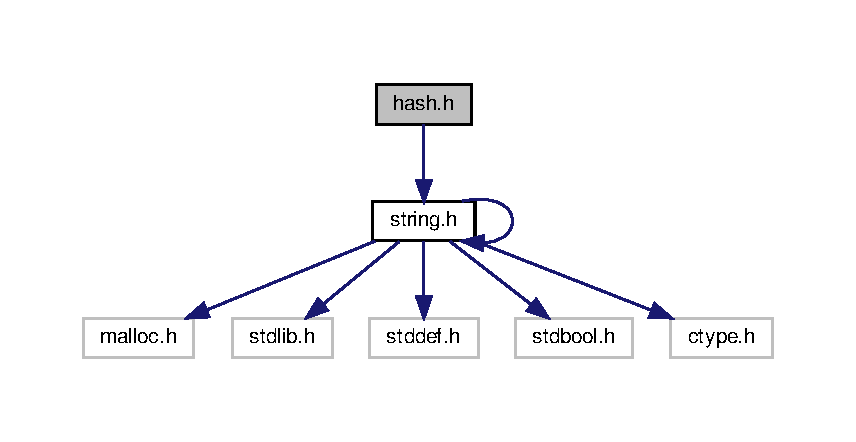
\includegraphics[width=350pt]{hash_8h__incl}
\end{center}
\end{figure}
This graph shows which files directly or indirectly include this file\+:
\nopagebreak
\begin{figure}[H]
\begin{center}
\leavevmode
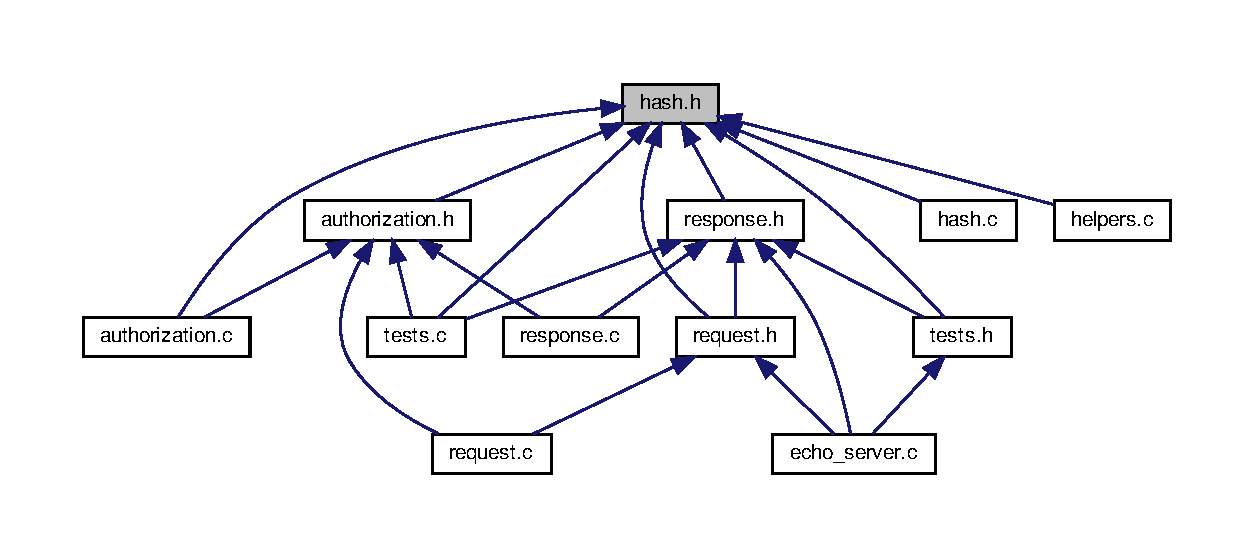
\includegraphics[width=350pt]{hash_8h__dep__incl}
\end{center}
\end{figure}
\subsection*{Data Structures}
\begin{DoxyCompactItemize}
\item 
struct \hyperlink{struct_string_hash_struct}{String\+Hash\+Struct}
\begin{DoxyCompactList}\small\item\em Hash element. \end{DoxyCompactList}\item 
struct \hyperlink{struct_string_hash_list}{String\+Hash\+List}
\begin{DoxyCompactList}\small\item\em Structure defining a list\+Element. \end{DoxyCompactList}\end{DoxyCompactItemize}
\subsection*{Typedefs}
\begin{DoxyCompactItemize}
\item 
typedef struct \hyperlink{struct_string_hash_struct}{String\+Hash\+Struct} \hyperlink{hash_8h_aaae8e320515f4ba6ab5e8bc4ecd7f58a}{Hash}
\begin{DoxyCompactList}\small\item\em Hash element. \end{DoxyCompactList}\item 
typedef struct \hyperlink{struct_string_hash_list}{String\+Hash\+List} \hyperlink{hash_8h_a58bb615f9115c5b9b1a49a64d3737edf}{Hash\+List}
\begin{DoxyCompactList}\small\item\em Structure defining a list\+Element. \end{DoxyCompactList}\end{DoxyCompactItemize}
\subsection*{Functions}
\begin{DoxyCompactItemize}
\item 
\hyperlink{hash_8h_a58bb615f9115c5b9b1a49a64d3737edf}{Hash\+List} $\ast$ \hyperlink{hash_8h_a73d7429aa205aee8b6e38808a8e2f53d}{S\+H\+L\+\_\+create} (\hyperlink{hash_8h_aaae8e320515f4ba6ab5e8bc4ecd7f58a}{Hash} first\+Element)
\begin{DoxyCompactList}\small\item\em creates new list Creates new list, but requires \end{DoxyCompactList}\item 
void \hyperlink{hash_8h_a5bf8ba8e50fdaedb05f2112695ec273c}{S\+H\+L\+\_\+append} (\hyperlink{hash_8h_a58bb615f9115c5b9b1a49a64d3737edf}{Hash\+List} $\ast$first, \hyperlink{hash_8h_aaae8e320515f4ba6ab5e8bc4ecd7f58a}{Hash} next)
\begin{DoxyCompactList}\small\item\em appends a new element at the end \end{DoxyCompactList}\item 
void \hyperlink{hash_8h_a7d3fe6343ca665e7014267c8f4905a9a}{S\+H\+L\+\_\+free\+\_\+element} (\hyperlink{hash_8h_a58bb615f9115c5b9b1a49a64d3737edf}{Hash\+List} $\ast$item)
\begin{DoxyCompactList}\small\item\em frees an element in the the list including it\textquotesingle{}s data\textquotesingle{}s Strings bear in mind that this will N\+OT touch the $\ast$next element \end{DoxyCompactList}\item 
void \hyperlink{hash_8h_a18f61bc4858ec37fc8f1198011c6b4e1}{S\+H\+L\+\_\+remove\+\_\+all} (\hyperlink{hash_8h_a58bb615f9115c5b9b1a49a64d3737edf}{Hash\+List} $\ast$first)
\begin{DoxyCompactList}\small\item\em removes element at position \end{DoxyCompactList}\item 
\hyperlink{hash_8h_aaae8e320515f4ba6ab5e8bc4ecd7f58a}{Hash} $\ast$ \hyperlink{hash_8h_a64a6c39375656b38732e8c3c20d2d9a0}{S\+H\+L\+\_\+find\+\_\+key} (\hyperlink{hash_8h_a58bb615f9115c5b9b1a49a64d3737edf}{Hash\+List} $\ast$first, \hyperlink{string_8h_a3d2981d9da3e25dd89371059777fdd12}{string} $\ast$key)
\begin{DoxyCompactList}\small\item\em returns pointer to the {\itshape F\+I\+R\+ST} element containing key Returns pointer to the {\itshape F\+I\+R\+ST} element containing key, will return N\+U\+LL if key is not found \end{DoxyCompactList}\item 
\hyperlink{hash_8h_aaae8e320515f4ba6ab5e8bc4ecd7f58a}{Hash} $\ast$ \hyperlink{hash_8h_ac084cf5afe24534957a0dc9ae964d054}{S\+H\+L\+\_\+find\+\_\+key\+\_\+cstr} (\hyperlink{hash_8h_a58bb615f9115c5b9b1a49a64d3737edf}{Hash\+List} $\ast$first, char $\ast$key)
\begin{DoxyCompactList}\small\item\em but with a char$\ast$ \end{DoxyCompactList}\item 
\hyperlink{hash_8h_aaae8e320515f4ba6ab5e8bc4ecd7f58a}{Hash} \hyperlink{hash_8h_ad0e07fdde374ab0435606a45dcdd58bc}{S\+H\+L\+\_\+at} (\hyperlink{hash_8h_a58bb615f9115c5b9b1a49a64d3737edf}{Hash\+List} $\ast$first, unsigned int index)
\begin{DoxyCompactList}\small\item\em return index\textquotesingle{}th element of Hash\+List function returning the index\textquotesingle{}th element of Hash\+List first, it will return the last element if index is out of bound \end{DoxyCompactList}\item 
size\+\_\+t \hyperlink{hash_8h_a1323eede38beba6ef99cda6b2538162b}{S\+H\+L\+\_\+get\+\_\+size} (\hyperlink{hash_8h_a58bb615f9115c5b9b1a49a64d3737edf}{Hash\+List} $\ast$first)
\begin{DoxyCompactList}\small\item\em function that counts the number of elements in the list beginning at first \end{DoxyCompactList}\item 
\hyperlink{hash_8h_aaae8e320515f4ba6ab5e8bc4ecd7f58a}{Hash} \hyperlink{hash_8h_af3a6014f24a682c18b619d581dd23db4}{S\+H\+\_\+create} (\hyperlink{string_8h_a3d2981d9da3e25dd89371059777fdd12}{string} $\ast$key, \hyperlink{string_8h_a3d2981d9da3e25dd89371059777fdd12}{string} $\ast$value)
\begin{DoxyCompactList}\small\item\em creates Hash with given key and value \end{DoxyCompactList}\end{DoxyCompactItemize}


\subsection{Detailed Description}
if you find spelling mistakes, keep them as trophy 

\begin{DoxyAuthor}{Author}
Björn Marx 
\end{DoxyAuthor}
\begin{DoxyDate}{Date}
12/04/2019. 
\end{DoxyDate}


\subsection{Typedef Documentation}
\mbox{\Hypertarget{hash_8h_aaae8e320515f4ba6ab5e8bc4ecd7f58a}\label{hash_8h_aaae8e320515f4ba6ab5e8bc4ecd7f58a}} 
\index{hash.\+h@{hash.\+h}!Hash@{Hash}}
\index{Hash@{Hash}!hash.\+h@{hash.\+h}}
\subsubsection{\texorpdfstring{Hash}{Hash}}
{\footnotesize\ttfamily typedef struct \hyperlink{struct_string_hash_struct}{String\+Hash\+Struct}  \hyperlink{hash_8h_aaae8e320515f4ba6ab5e8bc4ecd7f58a}{Hash}}



Hash element. 

\begin{DoxyAuthor}{Author}
Björn Marx 
\end{DoxyAuthor}
\mbox{\Hypertarget{hash_8h_a58bb615f9115c5b9b1a49a64d3737edf}\label{hash_8h_a58bb615f9115c5b9b1a49a64d3737edf}} 
\index{hash.\+h@{hash.\+h}!Hash\+List@{Hash\+List}}
\index{Hash\+List@{Hash\+List}!hash.\+h@{hash.\+h}}
\subsubsection{\texorpdfstring{Hash\+List}{HashList}}
{\footnotesize\ttfamily typedef struct \hyperlink{struct_string_hash_list}{String\+Hash\+List}  \hyperlink{hash_8h_a58bb615f9115c5b9b1a49a64d3737edf}{Hash\+List}}



Structure defining a list\+Element. 

\begin{DoxyAuthor}{Author}
Björn Marx 
\end{DoxyAuthor}


\subsection{Function Documentation}
\mbox{\Hypertarget{hash_8h_af3a6014f24a682c18b619d581dd23db4}\label{hash_8h_af3a6014f24a682c18b619d581dd23db4}} 
\index{hash.\+h@{hash.\+h}!S\+H\+\_\+create@{S\+H\+\_\+create}}
\index{S\+H\+\_\+create@{S\+H\+\_\+create}!hash.\+h@{hash.\+h}}
\subsubsection{\texorpdfstring{S\+H\+\_\+create()}{SH\_create()}}
{\footnotesize\ttfamily \hyperlink{hash_8h_aaae8e320515f4ba6ab5e8bc4ecd7f58a}{Hash} S\+H\+\_\+create (\begin{DoxyParamCaption}\item[{\hyperlink{string_8h_a3d2981d9da3e25dd89371059777fdd12}{string} $\ast$}]{key,  }\item[{\hyperlink{string_8h_a3d2981d9da3e25dd89371059777fdd12}{string} $\ast$}]{value }\end{DoxyParamCaption})}



creates Hash with given key and value 

\begin{DoxyAuthor}{Author}
Björn Marx
\end{DoxyAuthor}
\begin{DoxyReturn}{Returns}
copy of Hash with desired key and value 
\end{DoxyReturn}
\mbox{\Hypertarget{hash_8h_a5bf8ba8e50fdaedb05f2112695ec273c}\label{hash_8h_a5bf8ba8e50fdaedb05f2112695ec273c}} 
\index{hash.\+h@{hash.\+h}!S\+H\+L\+\_\+append@{S\+H\+L\+\_\+append}}
\index{S\+H\+L\+\_\+append@{S\+H\+L\+\_\+append}!hash.\+h@{hash.\+h}}
\subsubsection{\texorpdfstring{S\+H\+L\+\_\+append()}{SHL\_append()}}
{\footnotesize\ttfamily void S\+H\+L\+\_\+append (\begin{DoxyParamCaption}\item[{\hyperlink{hash_8h_a58bb615f9115c5b9b1a49a64d3737edf}{Hash\+List} $\ast$}]{first,  }\item[{\hyperlink{hash_8h_aaae8e320515f4ba6ab5e8bc4ecd7f58a}{Hash}}]{next }\end{DoxyParamCaption})}



appends a new element at the end 

\begin{DoxyAuthor}{Author}
Björn Marx 
\end{DoxyAuthor}
\mbox{\Hypertarget{hash_8h_ad0e07fdde374ab0435606a45dcdd58bc}\label{hash_8h_ad0e07fdde374ab0435606a45dcdd58bc}} 
\index{hash.\+h@{hash.\+h}!S\+H\+L\+\_\+at@{S\+H\+L\+\_\+at}}
\index{S\+H\+L\+\_\+at@{S\+H\+L\+\_\+at}!hash.\+h@{hash.\+h}}
\subsubsection{\texorpdfstring{S\+H\+L\+\_\+at()}{SHL\_at()}}
{\footnotesize\ttfamily \hyperlink{hash_8h_aaae8e320515f4ba6ab5e8bc4ecd7f58a}{Hash} S\+H\+L\+\_\+at (\begin{DoxyParamCaption}\item[{\hyperlink{hash_8h_a58bb615f9115c5b9b1a49a64d3737edf}{Hash\+List} $\ast$}]{first,  }\item[{unsigned int}]{index }\end{DoxyParamCaption})}



return index\textquotesingle{}th element of Hash\+List function returning the index\textquotesingle{}th element of Hash\+List first, it will return the last element if index is out of bound 

\begin{DoxyAuthor}{Author}
Björn Marx
\end{DoxyAuthor}

\begin{DoxyParams}{Parameters}
{\em first} & first element of list \\
\hline
{\em index} & index of desired element \\
\hline
\end{DoxyParams}
\begin{DoxyReturn}{Returns}
pointer to Hash object, will return last element if index ist out of range 
\end{DoxyReturn}
\mbox{\Hypertarget{hash_8h_a73d7429aa205aee8b6e38808a8e2f53d}\label{hash_8h_a73d7429aa205aee8b6e38808a8e2f53d}} 
\index{hash.\+h@{hash.\+h}!S\+H\+L\+\_\+create@{S\+H\+L\+\_\+create}}
\index{S\+H\+L\+\_\+create@{S\+H\+L\+\_\+create}!hash.\+h@{hash.\+h}}
\subsubsection{\texorpdfstring{S\+H\+L\+\_\+create()}{SHL\_create()}}
{\footnotesize\ttfamily \hyperlink{hash_8h_a58bb615f9115c5b9b1a49a64d3737edf}{Hash\+List}$\ast$ S\+H\+L\+\_\+create (\begin{DoxyParamCaption}\item[{\hyperlink{hash_8h_aaae8e320515f4ba6ab5e8bc4ecd7f58a}{Hash}}]{first\+Element }\end{DoxyParamCaption})}



creates new list Creates new list, but requires 

\begin{DoxyAuthor}{Author}
Björn Marx 
\end{DoxyAuthor}
\mbox{\Hypertarget{hash_8h_a64a6c39375656b38732e8c3c20d2d9a0}\label{hash_8h_a64a6c39375656b38732e8c3c20d2d9a0}} 
\index{hash.\+h@{hash.\+h}!S\+H\+L\+\_\+find\+\_\+key@{S\+H\+L\+\_\+find\+\_\+key}}
\index{S\+H\+L\+\_\+find\+\_\+key@{S\+H\+L\+\_\+find\+\_\+key}!hash.\+h@{hash.\+h}}
\subsubsection{\texorpdfstring{S\+H\+L\+\_\+find\+\_\+key()}{SHL\_find\_key()}}
{\footnotesize\ttfamily \hyperlink{hash_8h_aaae8e320515f4ba6ab5e8bc4ecd7f58a}{Hash}$\ast$ S\+H\+L\+\_\+find\+\_\+key (\begin{DoxyParamCaption}\item[{\hyperlink{hash_8h_a58bb615f9115c5b9b1a49a64d3737edf}{Hash\+List} $\ast$}]{first,  }\item[{\hyperlink{string_8h_a3d2981d9da3e25dd89371059777fdd12}{string} $\ast$}]{key }\end{DoxyParamCaption})}



returns pointer to the {\itshape F\+I\+R\+ST} element containing key Returns pointer to the {\itshape F\+I\+R\+ST} element containing key, will return N\+U\+LL if key is not found 

\begin{DoxyAuthor}{Author}
Björn Marx
\end{DoxyAuthor}

\begin{DoxyParams}{Parameters}
{\em first} & pointer to list \\
\hline
{\em key} & desired key to be found \\
\hline
\end{DoxyParams}
\begin{DoxyReturn}{Returns}
pointer to {\itshape first} element with key 
\end{DoxyReturn}
\mbox{\Hypertarget{hash_8h_ac084cf5afe24534957a0dc9ae964d054}\label{hash_8h_ac084cf5afe24534957a0dc9ae964d054}} 
\index{hash.\+h@{hash.\+h}!S\+H\+L\+\_\+find\+\_\+key\+\_\+cstr@{S\+H\+L\+\_\+find\+\_\+key\+\_\+cstr}}
\index{S\+H\+L\+\_\+find\+\_\+key\+\_\+cstr@{S\+H\+L\+\_\+find\+\_\+key\+\_\+cstr}!hash.\+h@{hash.\+h}}
\subsubsection{\texorpdfstring{S\+H\+L\+\_\+find\+\_\+key\+\_\+cstr()}{SHL\_find\_key\_cstr()}}
{\footnotesize\ttfamily \hyperlink{hash_8h_aaae8e320515f4ba6ab5e8bc4ecd7f58a}{Hash}$\ast$ S\+H\+L\+\_\+find\+\_\+key\+\_\+cstr (\begin{DoxyParamCaption}\item[{\hyperlink{hash_8h_a58bb615f9115c5b9b1a49a64d3737edf}{Hash\+List} $\ast$}]{first,  }\item[{char $\ast$}]{key }\end{DoxyParamCaption})}



but with a char$\ast$ 

\begin{DoxySeeAlso}{See also}
\hyperlink{hash_8h_a64a6c39375656b38732e8c3c20d2d9a0}{S\+H\+L\+\_\+find\+\_\+key} 
\end{DoxySeeAlso}
\mbox{\Hypertarget{hash_8h_a7d3fe6343ca665e7014267c8f4905a9a}\label{hash_8h_a7d3fe6343ca665e7014267c8f4905a9a}} 
\index{hash.\+h@{hash.\+h}!S\+H\+L\+\_\+free\+\_\+element@{S\+H\+L\+\_\+free\+\_\+element}}
\index{S\+H\+L\+\_\+free\+\_\+element@{S\+H\+L\+\_\+free\+\_\+element}!hash.\+h@{hash.\+h}}
\subsubsection{\texorpdfstring{S\+H\+L\+\_\+free\+\_\+element()}{SHL\_free\_element()}}
{\footnotesize\ttfamily void S\+H\+L\+\_\+free\+\_\+element (\begin{DoxyParamCaption}\item[{\hyperlink{hash_8h_a58bb615f9115c5b9b1a49a64d3737edf}{Hash\+List} $\ast$}]{item }\end{DoxyParamCaption})}



frees an element in the the list including it\textquotesingle{}s data\textquotesingle{}s Strings bear in mind that this will N\+OT touch the $\ast$next element 

\begin{DoxyAuthor}{Author}
Björn Marx
\end{DoxyAuthor}

\begin{DoxyParams}{Parameters}
{\em item} & the list element that shall be freed \\
\hline
\end{DoxyParams}
\mbox{\Hypertarget{hash_8h_a1323eede38beba6ef99cda6b2538162b}\label{hash_8h_a1323eede38beba6ef99cda6b2538162b}} 
\index{hash.\+h@{hash.\+h}!S\+H\+L\+\_\+get\+\_\+size@{S\+H\+L\+\_\+get\+\_\+size}}
\index{S\+H\+L\+\_\+get\+\_\+size@{S\+H\+L\+\_\+get\+\_\+size}!hash.\+h@{hash.\+h}}
\subsubsection{\texorpdfstring{S\+H\+L\+\_\+get\+\_\+size()}{SHL\_get\_size()}}
{\footnotesize\ttfamily size\+\_\+t S\+H\+L\+\_\+get\+\_\+size (\begin{DoxyParamCaption}\item[{\hyperlink{hash_8h_a58bb615f9115c5b9b1a49a64d3737edf}{Hash\+List} $\ast$}]{first }\end{DoxyParamCaption})}



function that counts the number of elements in the list beginning at first 


\begin{DoxyParams}{Parameters}
{\em first} & first list element \\
\hline
\end{DoxyParams}
\begin{DoxyReturn}{Returns}
size of Hashlist 
\end{DoxyReturn}
\mbox{\Hypertarget{hash_8h_a18f61bc4858ec37fc8f1198011c6b4e1}\label{hash_8h_a18f61bc4858ec37fc8f1198011c6b4e1}} 
\index{hash.\+h@{hash.\+h}!S\+H\+L\+\_\+remove\+\_\+all@{S\+H\+L\+\_\+remove\+\_\+all}}
\index{S\+H\+L\+\_\+remove\+\_\+all@{S\+H\+L\+\_\+remove\+\_\+all}!hash.\+h@{hash.\+h}}
\subsubsection{\texorpdfstring{S\+H\+L\+\_\+remove\+\_\+all()}{SHL\_remove\_all()}}
{\footnotesize\ttfamily void S\+H\+L\+\_\+remove\+\_\+all (\begin{DoxyParamCaption}\item[{\hyperlink{hash_8h_a58bb615f9115c5b9b1a49a64d3737edf}{Hash\+List} $\ast$}]{first }\end{DoxyParamCaption})}



removes element at position 

\begin{DoxyAuthor}{Author}
Björn Marx
\end{DoxyAuthor}

\begin{DoxyParams}{Parameters}
{\em first} & pointer to fist list element\\
\hline
\end{DoxyParams}
deletes all elements starting at first

\begin{DoxyAuthor}{Author}
Björn Marx 
\end{DoxyAuthor}

\hypertarget{helpers_8c}{}\section{helpers.\+c File Reference}
\label{helpers_8c}\index{helpers.\+c@{helpers.\+c}}
{\ttfamily \#include \char`\"{}helpers.\+h\char`\"{}}\newline
{\ttfamily \#include \char`\"{}hash.\+h\char`\"{}}\newline
Include dependency graph for helpers.\+c\+:
\nopagebreak
\begin{figure}[H]
\begin{center}
\leavevmode
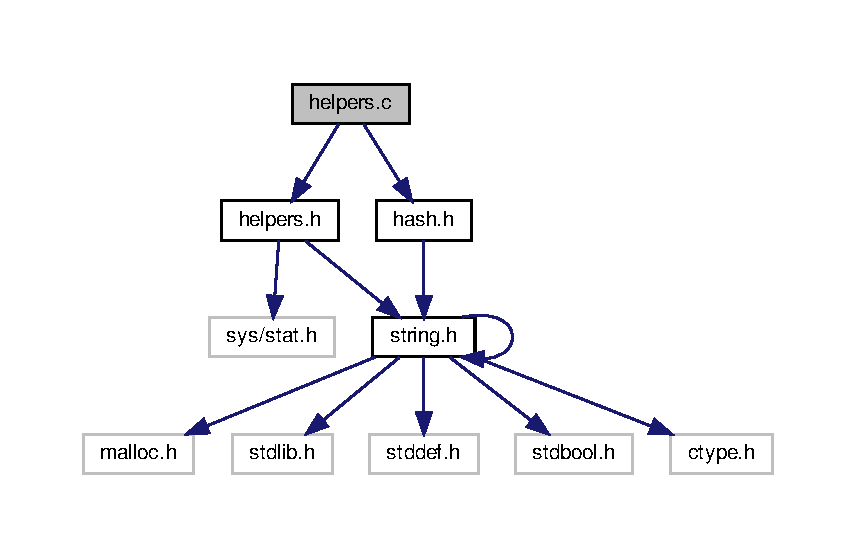
\includegraphics[width=350pt]{helpers_8c__incl}
\end{center}
\end{figure}
\subsection*{Functions}
\begin{DoxyCompactItemize}
\item 
\hyperlink{string_8h_a3d2981d9da3e25dd89371059777fdd12}{string} $\ast$ \hyperlink{helpers_8c_a90c8a390258292e7ee1c47d262de3c45}{get\+\_\+content\+\_\+type} (char $\ast$path)
\begin{DoxyCompactList}\small\item\em gets content type of file with help of the file command \end{DoxyCompactList}\item 
void \hyperlink{helpers_8c_ac2c0d16dc3ce1f1ff1d1bf0b674a55fb}{url\+\_\+decode} (\hyperlink{string_8h_a3d2981d9da3e25dd89371059777fdd12}{string} $\ast$str)
\begin{DoxyCompactList}\small\item\em decodes url, obviously \end{DoxyCompactList}\item 
\hyperlink{helpers_8h_abe818f5ff14e9c60c052a3e96877cec6}{H\+T\+T\+P\+Version} \hyperlink{helpers_8c_a224628953b1df47560e39e7d8056023b}{validate\+\_\+version} (\hyperlink{string_8h_a3d2981d9da3e25dd89371059777fdd12}{string} $\ast$ver)
\begin{DoxyCompactList}\small\item\em checks whether the H\+T\+TP version is supported or not note that the string must be valid by H\+T\+TP header standard (\char`\"{}\+H\+T\+T\+P/1.\+1\char`\"{}, others not supported) \end{DoxyCompactList}\item 
\hyperlink{helpers_8h_a837a089a977b319a11edfb8022d9e47d}{H\+T\+T\+P\+Method} \hyperlink{helpers_8c_abb0d6160f45c0b3f86392f93d3e84a8a}{get\+\_\+method\+\_\+from\+\_\+string} (\hyperlink{string_8h_a3d2981d9da3e25dd89371059777fdd12}{string} $\ast$method)
\begin{DoxyCompactList}\small\item\em gets the H\+T\+TP method from a string \end{DoxyCompactList}\item 
bool \hyperlink{helpers_8c_a3ada2da8156daa4803e778aa6d5e8953}{isfile} (\hyperlink{string_8h_a3d2981d9da3e25dd89371059777fdd12}{string} $\ast$path)
\begin{DoxyCompactList}\small\item\em checks if a given path is a file \end{DoxyCompactList}\item 
bool \hyperlink{helpers_8c_ab7a73667739cc6fa285e8d4c6205eb9b}{file\+\_\+exists} (\hyperlink{string_8h_a3d2981d9da3e25dd89371059777fdd12}{string} $\ast$path)
\begin{DoxyCompactList}\small\item\em checks if a file exists \end{DoxyCompactList}\item 
long \hyperlink{helpers_8c_a503cd4ef941c2395f50e1cb089626882}{get\+\_\+file\+\_\+size} (F\+I\+LE $\ast$fp)
\begin{DoxyCompactList}\small\item\em returns the file size of a opened file (with fopen) \end{DoxyCompactList}\end{DoxyCompactItemize}


\subsection{Function Documentation}
\mbox{\Hypertarget{helpers_8c_ab7a73667739cc6fa285e8d4c6205eb9b}\label{helpers_8c_ab7a73667739cc6fa285e8d4c6205eb9b}} 
\index{helpers.\+c@{helpers.\+c}!file\+\_\+exists@{file\+\_\+exists}}
\index{file\+\_\+exists@{file\+\_\+exists}!helpers.\+c@{helpers.\+c}}
\subsubsection{\texorpdfstring{file\+\_\+exists()}{file\_exists()}}
{\footnotesize\ttfamily bool file\+\_\+exists (\begin{DoxyParamCaption}\item[{\hyperlink{string_8h_a3d2981d9da3e25dd89371059777fdd12}{string} $\ast$}]{path }\end{DoxyParamCaption})}



checks if a file exists 

\begin{DoxyAuthor}{Author}
Marcel Weski 
\end{DoxyAuthor}

\begin{DoxyParams}{Parameters}
{\em path} & filepath \\
\hline
\end{DoxyParams}
\begin{DoxyReturn}{Returns}
true if file exists 
\end{DoxyReturn}
\mbox{\Hypertarget{helpers_8c_a90c8a390258292e7ee1c47d262de3c45}\label{helpers_8c_a90c8a390258292e7ee1c47d262de3c45}} 
\index{helpers.\+c@{helpers.\+c}!get\+\_\+content\+\_\+type@{get\+\_\+content\+\_\+type}}
\index{get\+\_\+content\+\_\+type@{get\+\_\+content\+\_\+type}!helpers.\+c@{helpers.\+c}}
\subsubsection{\texorpdfstring{get\+\_\+content\+\_\+type()}{get\_content\_type()}}
{\footnotesize\ttfamily \hyperlink{string_8h_a3d2981d9da3e25dd89371059777fdd12}{string}$\ast$ get\+\_\+content\+\_\+type (\begin{DoxyParamCaption}\item[{char $\ast$}]{path }\end{DoxyParamCaption})}



gets content type of file with help of the file command 

\begin{DoxyWarning}{Warning}
as it seems to be forgotten otherwise\+: Y\+OU H\+A\+VE TO F\+R\+EE T\+HE R\+E\+T\+U\+R\+N\+ED S\+T\+R\+I\+NG Y\+O\+U\+R\+S\+E\+L\+F!
\end{DoxyWarning}
\begin{DoxyAuthor}{Author}
Björn Marx
\end{DoxyAuthor}

\begin{DoxyParams}{Parameters}
{\em path} & path to file \\
\hline
\end{DoxyParams}
\begin{DoxyReturn}{Returns}
content type and charset as string, separated by \textquotesingle{};\textquotesingle{} 
\end{DoxyReturn}
\mbox{\Hypertarget{helpers_8c_a503cd4ef941c2395f50e1cb089626882}\label{helpers_8c_a503cd4ef941c2395f50e1cb089626882}} 
\index{helpers.\+c@{helpers.\+c}!get\+\_\+file\+\_\+size@{get\+\_\+file\+\_\+size}}
\index{get\+\_\+file\+\_\+size@{get\+\_\+file\+\_\+size}!helpers.\+c@{helpers.\+c}}
\subsubsection{\texorpdfstring{get\+\_\+file\+\_\+size()}{get\_file\_size()}}
{\footnotesize\ttfamily long get\+\_\+file\+\_\+size (\begin{DoxyParamCaption}\item[{F\+I\+LE $\ast$}]{fp }\end{DoxyParamCaption})}



returns the file size of a opened file (with fopen) 

\begin{DoxyAuthor}{Author}
Marcel Weski 
\end{DoxyAuthor}

\begin{DoxyParams}{Parameters}
{\em fp} & pointer of opened file \\
\hline
\end{DoxyParams}
\begin{DoxyReturn}{Returns}
file size 
\end{DoxyReturn}
\mbox{\Hypertarget{helpers_8c_abb0d6160f45c0b3f86392f93d3e84a8a}\label{helpers_8c_abb0d6160f45c0b3f86392f93d3e84a8a}} 
\index{helpers.\+c@{helpers.\+c}!get\+\_\+method\+\_\+from\+\_\+string@{get\+\_\+method\+\_\+from\+\_\+string}}
\index{get\+\_\+method\+\_\+from\+\_\+string@{get\+\_\+method\+\_\+from\+\_\+string}!helpers.\+c@{helpers.\+c}}
\subsubsection{\texorpdfstring{get\+\_\+method\+\_\+from\+\_\+string()}{get\_method\_from\_string()}}
{\footnotesize\ttfamily \hyperlink{helpers_8h_a837a089a977b319a11edfb8022d9e47d}{H\+T\+T\+P\+Method} get\+\_\+method\+\_\+from\+\_\+string (\begin{DoxyParamCaption}\item[{\hyperlink{string_8h_a3d2981d9da3e25dd89371059777fdd12}{string} $\ast$}]{method }\end{DoxyParamCaption})}



gets the H\+T\+TP method from a string 

\begin{DoxyAuthor}{Author}
Björn Marx
\end{DoxyAuthor}

\begin{DoxyParams}{Parameters}
{\em method} & string containing the method \\
\hline
\end{DoxyParams}
\begin{DoxyReturn}{Returns}
Method or Invalid 
\end{DoxyReturn}
\mbox{\Hypertarget{helpers_8c_a3ada2da8156daa4803e778aa6d5e8953}\label{helpers_8c_a3ada2da8156daa4803e778aa6d5e8953}} 
\index{helpers.\+c@{helpers.\+c}!isfile@{isfile}}
\index{isfile@{isfile}!helpers.\+c@{helpers.\+c}}
\subsubsection{\texorpdfstring{isfile()}{isfile()}}
{\footnotesize\ttfamily bool isfile (\begin{DoxyParamCaption}\item[{\hyperlink{string_8h_a3d2981d9da3e25dd89371059777fdd12}{string} $\ast$}]{path }\end{DoxyParamCaption})}



checks if a given path is a file 

\begin{DoxyAuthor}{Author}
Marcel Weski 
\end{DoxyAuthor}

\begin{DoxyParams}{Parameters}
{\em path} & path of file or directory \\
\hline
\end{DoxyParams}
\begin{DoxyReturn}{Returns}
true if path is a existing file 
\end{DoxyReturn}
\mbox{\Hypertarget{helpers_8c_ac2c0d16dc3ce1f1ff1d1bf0b674a55fb}\label{helpers_8c_ac2c0d16dc3ce1f1ff1d1bf0b674a55fb}} 
\index{helpers.\+c@{helpers.\+c}!url\+\_\+decode@{url\+\_\+decode}}
\index{url\+\_\+decode@{url\+\_\+decode}!helpers.\+c@{helpers.\+c}}
\subsubsection{\texorpdfstring{url\+\_\+decode()}{url\_decode()}}
{\footnotesize\ttfamily void url\+\_\+decode (\begin{DoxyParamCaption}\item[{\hyperlink{string_8h_a3d2981d9da3e25dd89371059777fdd12}{string} $\ast$}]{str }\end{DoxyParamCaption})}



decodes url, obviously 

replaces the xx placeholder from H\+T\+ML with their corresponding ascii chars

\begin{DoxyAuthor}{Author}
Björn Marx
\end{DoxyAuthor}

\begin{DoxyParams}{Parameters}
{\em str} & a string with html\textquotesingle{}s weird XX placeholders \\
\hline
\end{DoxyParams}
\mbox{\Hypertarget{helpers_8c_a224628953b1df47560e39e7d8056023b}\label{helpers_8c_a224628953b1df47560e39e7d8056023b}} 
\index{helpers.\+c@{helpers.\+c}!validate\+\_\+version@{validate\+\_\+version}}
\index{validate\+\_\+version@{validate\+\_\+version}!helpers.\+c@{helpers.\+c}}
\subsubsection{\texorpdfstring{validate\+\_\+version()}{validate\_version()}}
{\footnotesize\ttfamily \hyperlink{helpers_8h_abe818f5ff14e9c60c052a3e96877cec6}{H\+T\+T\+P\+Version} validate\+\_\+version (\begin{DoxyParamCaption}\item[{\hyperlink{string_8h_a3d2981d9da3e25dd89371059777fdd12}{string} $\ast$}]{ver }\end{DoxyParamCaption})}



checks whether the H\+T\+TP version is supported or not note that the string must be valid by H\+T\+TP header standard (\char`\"{}\+H\+T\+T\+P/1.\+1\char`\"{}, others not supported) 

\begin{DoxyAuthor}{Author}
Björn Marx
\end{DoxyAuthor}

\begin{DoxyParams}{Parameters}
{\em ver} & a string containing the H\+T\+TP version \\
\hline
\end{DoxyParams}
\begin{DoxyReturn}{Returns}
Version or unsupported 
\end{DoxyReturn}

\hypertarget{helpers_8h}{}\section{helpers.\+h File Reference}
\label{helpers_8h}\index{helpers.\+h@{helpers.\+h}}
{\ttfamily \#include $<$sys/stat.\+h$>$}\newline
{\ttfamily \#include \char`\"{}string.\+h\char`\"{}}\newline
Include dependency graph for helpers.\+h\+:
\nopagebreak
\begin{figure}[H]
\begin{center}
\leavevmode
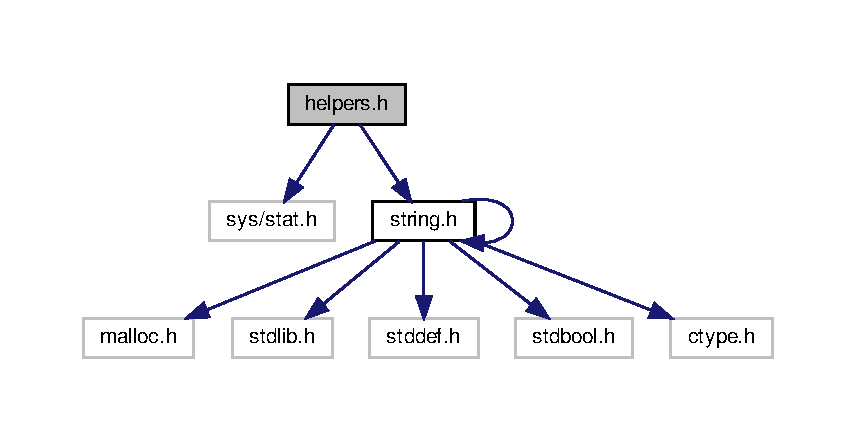
\includegraphics[width=350pt]{helpers_8h__incl}
\end{center}
\end{figure}
This graph shows which files directly or indirectly include this file\+:
\nopagebreak
\begin{figure}[H]
\begin{center}
\leavevmode
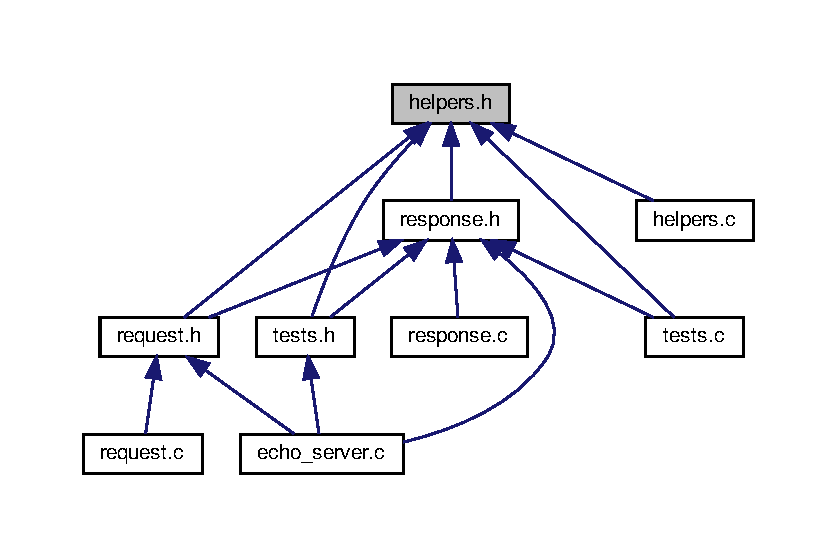
\includegraphics[width=350pt]{helpers_8h__dep__incl}
\end{center}
\end{figure}
\subsection*{Enumerations}
\begin{DoxyCompactItemize}
\item 
enum \hyperlink{helpers_8h_abe818f5ff14e9c60c052a3e96877cec6}{H\+T\+T\+P\+Version} \{ \hyperlink{helpers_8h_abe818f5ff14e9c60c052a3e96877cec6adb29f51e8818eebf58eaf92ba47467c9}{U\+N\+S\+U\+P\+P\+O\+R\+T\+ED}, 
\hyperlink{helpers_8h_abe818f5ff14e9c60c052a3e96877cec6ac121049d53f4061ca94d91084f73892a}{V\+E\+R\+S\+I\+O\+N\+\_\+1\+\_\+1}
 \}\begin{DoxyCompactList}\small\item\em enum containing supported version(s) \end{DoxyCompactList}
\item 
enum \hyperlink{helpers_8h_a837a089a977b319a11edfb8022d9e47d}{H\+T\+T\+P\+Method} \{ \newline
\hyperlink{helpers_8h_a837a089a977b319a11edfb8022d9e47daef2863a469df3ea6871d640e3669a2f2}{I\+N\+V\+A\+L\+ID}, 
\hyperlink{helpers_8h_a837a089a977b319a11edfb8022d9e47da12a8dcf59c16b5aadfda3a08ba67d529}{G\+ET}, 
\hyperlink{helpers_8h_a837a089a977b319a11edfb8022d9e47da368c5bc07109370b819193871352b926}{P\+O\+ST}, 
\hyperlink{helpers_8h_a837a089a977b319a11edfb8022d9e47da0b0955668575b21eb0ab2272aef49f76}{H\+E\+AD}, 
\newline
\hyperlink{helpers_8h_a837a089a977b319a11edfb8022d9e47dafec39d40e8bc9e12afa614df5ddb9fa9}{P\+UT}, 
\hyperlink{helpers_8h_a837a089a977b319a11edfb8022d9e47da8968cec66e1a913f0ef4d1205a7bf098}{P\+A\+T\+CH}, 
\hyperlink{helpers_8h_a837a089a977b319a11edfb8022d9e47da9d61e82a9a12752f10aece1b22183913}{D\+E\+L\+E\+TE}, 
\hyperlink{helpers_8h_a837a089a977b319a11edfb8022d9e47da7fa27e82c6c4f69434225ed81e5d151e}{T\+R\+A\+CE}, 
\newline
\hyperlink{helpers_8h_a837a089a977b319a11edfb8022d9e47da1b20f1b4adb6ff9778b284fb46f6f99d}{O\+P\+T\+I\+O\+NS}, 
\hyperlink{helpers_8h_a837a089a977b319a11edfb8022d9e47da20391dd2915a0e64343d24c2f2e40b95}{C\+O\+N\+N\+E\+CT}
 \}\begin{DoxyCompactList}\small\item\em enum containing supported methods \end{DoxyCompactList}
\end{DoxyCompactItemize}
\subsection*{Functions}
\begin{DoxyCompactItemize}
\item 
\hyperlink{helpers_8h_abe818f5ff14e9c60c052a3e96877cec6}{H\+T\+T\+P\+Version} \hyperlink{helpers_8h_a224628953b1df47560e39e7d8056023b}{validate\+\_\+version} (\hyperlink{string_8h_a3d2981d9da3e25dd89371059777fdd12}{string} $\ast$ver)
\begin{DoxyCompactList}\small\item\em checks whether the H\+T\+TP version is supported or not note that the string must be valid by H\+T\+TP header standard (\char`\"{}\+H\+T\+T\+P/1.\+1\char`\"{}, others not supported) \end{DoxyCompactList}\item 
\hyperlink{helpers_8h_a837a089a977b319a11edfb8022d9e47d}{H\+T\+T\+P\+Method} \hyperlink{helpers_8h_abb0d6160f45c0b3f86392f93d3e84a8a}{get\+\_\+method\+\_\+from\+\_\+string} (\hyperlink{string_8h_a3d2981d9da3e25dd89371059777fdd12}{string} $\ast$method)
\begin{DoxyCompactList}\small\item\em gets the H\+T\+TP method from a string \end{DoxyCompactList}\item 
\hyperlink{string_8h_a3d2981d9da3e25dd89371059777fdd12}{string} $\ast$ \hyperlink{helpers_8h_a90c8a390258292e7ee1c47d262de3c45}{get\+\_\+content\+\_\+type} (char $\ast$path)
\begin{DoxyCompactList}\small\item\em gets content type of file with help of the file command \end{DoxyCompactList}\item 
void \hyperlink{helpers_8h_ac2c0d16dc3ce1f1ff1d1bf0b674a55fb}{url\+\_\+decode} (\hyperlink{string_8h_a3d2981d9da3e25dd89371059777fdd12}{string} $\ast$str)
\begin{DoxyCompactList}\small\item\em decodes url, obviously \end{DoxyCompactList}\item 
bool \hyperlink{helpers_8h_a3ada2da8156daa4803e778aa6d5e8953}{isfile} (\hyperlink{string_8h_a3d2981d9da3e25dd89371059777fdd12}{string} $\ast$path)
\begin{DoxyCompactList}\small\item\em checks if a given path is a file \end{DoxyCompactList}\item 
bool \hyperlink{helpers_8h_ab7a73667739cc6fa285e8d4c6205eb9b}{file\+\_\+exists} (\hyperlink{string_8h_a3d2981d9da3e25dd89371059777fdd12}{string} $\ast$path)
\begin{DoxyCompactList}\small\item\em checks if a file exists \end{DoxyCompactList}\item 
long \hyperlink{helpers_8h_a503cd4ef941c2395f50e1cb089626882}{get\+\_\+file\+\_\+size} (F\+I\+LE $\ast$fp)
\begin{DoxyCompactList}\small\item\em returns the file size of a opened file (with fopen) \end{DoxyCompactList}\end{DoxyCompactItemize}


\subsection{Detailed Description}
\begin{DoxyAuthor}{Author}
Björn Marx 
\end{DoxyAuthor}


\subsection{Enumeration Type Documentation}
\mbox{\Hypertarget{helpers_8h_a837a089a977b319a11edfb8022d9e47d}\label{helpers_8h_a837a089a977b319a11edfb8022d9e47d}} 
\index{helpers.\+h@{helpers.\+h}!H\+T\+T\+P\+Method@{H\+T\+T\+P\+Method}}
\index{H\+T\+T\+P\+Method@{H\+T\+T\+P\+Method}!helpers.\+h@{helpers.\+h}}
\subsubsection{\texorpdfstring{H\+T\+T\+P\+Method}{HTTPMethod}}
{\footnotesize\ttfamily enum \hyperlink{helpers_8h_a837a089a977b319a11edfb8022d9e47d}{H\+T\+T\+P\+Method}}



enum containing supported methods 

\begin{DoxyAuthor}{Author}
Björn Marx 
\end{DoxyAuthor}
\begin{DoxyEnumFields}{Enumerator}
\raisebox{\heightof{T}}[0pt][0pt]{\index{I\+N\+V\+A\+L\+ID@{I\+N\+V\+A\+L\+ID}!helpers.\+h@{helpers.\+h}}\index{helpers.\+h@{helpers.\+h}!I\+N\+V\+A\+L\+ID@{I\+N\+V\+A\+L\+ID}}}\mbox{\Hypertarget{helpers_8h_a837a089a977b319a11edfb8022d9e47daef2863a469df3ea6871d640e3669a2f2}\label{helpers_8h_a837a089a977b319a11edfb8022d9e47daef2863a469df3ea6871d640e3669a2f2}} 
I\+N\+V\+A\+L\+ID&\\
\hline

\raisebox{\heightof{T}}[0pt][0pt]{\index{G\+ET@{G\+ET}!helpers.\+h@{helpers.\+h}}\index{helpers.\+h@{helpers.\+h}!G\+ET@{G\+ET}}}\mbox{\Hypertarget{helpers_8h_a837a089a977b319a11edfb8022d9e47da12a8dcf59c16b5aadfda3a08ba67d529}\label{helpers_8h_a837a089a977b319a11edfb8022d9e47da12a8dcf59c16b5aadfda3a08ba67d529}} 
G\+ET&\\
\hline

\raisebox{\heightof{T}}[0pt][0pt]{\index{P\+O\+ST@{P\+O\+ST}!helpers.\+h@{helpers.\+h}}\index{helpers.\+h@{helpers.\+h}!P\+O\+ST@{P\+O\+ST}}}\mbox{\Hypertarget{helpers_8h_a837a089a977b319a11edfb8022d9e47da368c5bc07109370b819193871352b926}\label{helpers_8h_a837a089a977b319a11edfb8022d9e47da368c5bc07109370b819193871352b926}} 
P\+O\+ST&\\
\hline

\raisebox{\heightof{T}}[0pt][0pt]{\index{H\+E\+AD@{H\+E\+AD}!helpers.\+h@{helpers.\+h}}\index{helpers.\+h@{helpers.\+h}!H\+E\+AD@{H\+E\+AD}}}\mbox{\Hypertarget{helpers_8h_a837a089a977b319a11edfb8022d9e47da0b0955668575b21eb0ab2272aef49f76}\label{helpers_8h_a837a089a977b319a11edfb8022d9e47da0b0955668575b21eb0ab2272aef49f76}} 
H\+E\+AD&\\
\hline

\raisebox{\heightof{T}}[0pt][0pt]{\index{P\+UT@{P\+UT}!helpers.\+h@{helpers.\+h}}\index{helpers.\+h@{helpers.\+h}!P\+UT@{P\+UT}}}\mbox{\Hypertarget{helpers_8h_a837a089a977b319a11edfb8022d9e47dafec39d40e8bc9e12afa614df5ddb9fa9}\label{helpers_8h_a837a089a977b319a11edfb8022d9e47dafec39d40e8bc9e12afa614df5ddb9fa9}} 
P\+UT&\\
\hline

\raisebox{\heightof{T}}[0pt][0pt]{\index{P\+A\+T\+CH@{P\+A\+T\+CH}!helpers.\+h@{helpers.\+h}}\index{helpers.\+h@{helpers.\+h}!P\+A\+T\+CH@{P\+A\+T\+CH}}}\mbox{\Hypertarget{helpers_8h_a837a089a977b319a11edfb8022d9e47da8968cec66e1a913f0ef4d1205a7bf098}\label{helpers_8h_a837a089a977b319a11edfb8022d9e47da8968cec66e1a913f0ef4d1205a7bf098}} 
P\+A\+T\+CH&\\
\hline

\raisebox{\heightof{T}}[0pt][0pt]{\index{D\+E\+L\+E\+TE@{D\+E\+L\+E\+TE}!helpers.\+h@{helpers.\+h}}\index{helpers.\+h@{helpers.\+h}!D\+E\+L\+E\+TE@{D\+E\+L\+E\+TE}}}\mbox{\Hypertarget{helpers_8h_a837a089a977b319a11edfb8022d9e47da9d61e82a9a12752f10aece1b22183913}\label{helpers_8h_a837a089a977b319a11edfb8022d9e47da9d61e82a9a12752f10aece1b22183913}} 
D\+E\+L\+E\+TE&\\
\hline

\raisebox{\heightof{T}}[0pt][0pt]{\index{T\+R\+A\+CE@{T\+R\+A\+CE}!helpers.\+h@{helpers.\+h}}\index{helpers.\+h@{helpers.\+h}!T\+R\+A\+CE@{T\+R\+A\+CE}}}\mbox{\Hypertarget{helpers_8h_a837a089a977b319a11edfb8022d9e47da7fa27e82c6c4f69434225ed81e5d151e}\label{helpers_8h_a837a089a977b319a11edfb8022d9e47da7fa27e82c6c4f69434225ed81e5d151e}} 
T\+R\+A\+CE&\\
\hline

\raisebox{\heightof{T}}[0pt][0pt]{\index{O\+P\+T\+I\+O\+NS@{O\+P\+T\+I\+O\+NS}!helpers.\+h@{helpers.\+h}}\index{helpers.\+h@{helpers.\+h}!O\+P\+T\+I\+O\+NS@{O\+P\+T\+I\+O\+NS}}}\mbox{\Hypertarget{helpers_8h_a837a089a977b319a11edfb8022d9e47da1b20f1b4adb6ff9778b284fb46f6f99d}\label{helpers_8h_a837a089a977b319a11edfb8022d9e47da1b20f1b4adb6ff9778b284fb46f6f99d}} 
O\+P\+T\+I\+O\+NS&\\
\hline

\raisebox{\heightof{T}}[0pt][0pt]{\index{C\+O\+N\+N\+E\+CT@{C\+O\+N\+N\+E\+CT}!helpers.\+h@{helpers.\+h}}\index{helpers.\+h@{helpers.\+h}!C\+O\+N\+N\+E\+CT@{C\+O\+N\+N\+E\+CT}}}\mbox{\Hypertarget{helpers_8h_a837a089a977b319a11edfb8022d9e47da20391dd2915a0e64343d24c2f2e40b95}\label{helpers_8h_a837a089a977b319a11edfb8022d9e47da20391dd2915a0e64343d24c2f2e40b95}} 
C\+O\+N\+N\+E\+CT&\\
\hline

\end{DoxyEnumFields}
\mbox{\Hypertarget{helpers_8h_abe818f5ff14e9c60c052a3e96877cec6}\label{helpers_8h_abe818f5ff14e9c60c052a3e96877cec6}} 
\index{helpers.\+h@{helpers.\+h}!H\+T\+T\+P\+Version@{H\+T\+T\+P\+Version}}
\index{H\+T\+T\+P\+Version@{H\+T\+T\+P\+Version}!helpers.\+h@{helpers.\+h}}
\subsubsection{\texorpdfstring{H\+T\+T\+P\+Version}{HTTPVersion}}
{\footnotesize\ttfamily enum \hyperlink{helpers_8h_abe818f5ff14e9c60c052a3e96877cec6}{H\+T\+T\+P\+Version}}



enum containing supported version(s) 

\begin{DoxyAuthor}{Author}
Björn Marx 
\end{DoxyAuthor}
\begin{DoxyEnumFields}{Enumerator}
\raisebox{\heightof{T}}[0pt][0pt]{\index{U\+N\+S\+U\+P\+P\+O\+R\+T\+ED@{U\+N\+S\+U\+P\+P\+O\+R\+T\+ED}!helpers.\+h@{helpers.\+h}}\index{helpers.\+h@{helpers.\+h}!U\+N\+S\+U\+P\+P\+O\+R\+T\+ED@{U\+N\+S\+U\+P\+P\+O\+R\+T\+ED}}}\mbox{\Hypertarget{helpers_8h_abe818f5ff14e9c60c052a3e96877cec6adb29f51e8818eebf58eaf92ba47467c9}\label{helpers_8h_abe818f5ff14e9c60c052a3e96877cec6adb29f51e8818eebf58eaf92ba47467c9}} 
U\+N\+S\+U\+P\+P\+O\+R\+T\+ED&\\
\hline

\raisebox{\heightof{T}}[0pt][0pt]{\index{V\+E\+R\+S\+I\+O\+N\+\_\+1\+\_\+1@{V\+E\+R\+S\+I\+O\+N\+\_\+1\+\_\+1}!helpers.\+h@{helpers.\+h}}\index{helpers.\+h@{helpers.\+h}!V\+E\+R\+S\+I\+O\+N\+\_\+1\+\_\+1@{V\+E\+R\+S\+I\+O\+N\+\_\+1\+\_\+1}}}\mbox{\Hypertarget{helpers_8h_abe818f5ff14e9c60c052a3e96877cec6ac121049d53f4061ca94d91084f73892a}\label{helpers_8h_abe818f5ff14e9c60c052a3e96877cec6ac121049d53f4061ca94d91084f73892a}} 
V\+E\+R\+S\+I\+O\+N\+\_\+1\+\_\+1&\\
\hline

\end{DoxyEnumFields}


\subsection{Function Documentation}
\mbox{\Hypertarget{helpers_8h_ab7a73667739cc6fa285e8d4c6205eb9b}\label{helpers_8h_ab7a73667739cc6fa285e8d4c6205eb9b}} 
\index{helpers.\+h@{helpers.\+h}!file\+\_\+exists@{file\+\_\+exists}}
\index{file\+\_\+exists@{file\+\_\+exists}!helpers.\+h@{helpers.\+h}}
\subsubsection{\texorpdfstring{file\+\_\+exists()}{file\_exists()}}
{\footnotesize\ttfamily bool file\+\_\+exists (\begin{DoxyParamCaption}\item[{\hyperlink{string_8h_a3d2981d9da3e25dd89371059777fdd12}{string} $\ast$}]{path }\end{DoxyParamCaption})}



checks if a file exists 

\begin{DoxyAuthor}{Author}
Marcel Weski 
\end{DoxyAuthor}

\begin{DoxyParams}{Parameters}
{\em path} & filepath \\
\hline
\end{DoxyParams}
\begin{DoxyReturn}{Returns}
true if file exists 
\end{DoxyReturn}
\mbox{\Hypertarget{helpers_8h_a90c8a390258292e7ee1c47d262de3c45}\label{helpers_8h_a90c8a390258292e7ee1c47d262de3c45}} 
\index{helpers.\+h@{helpers.\+h}!get\+\_\+content\+\_\+type@{get\+\_\+content\+\_\+type}}
\index{get\+\_\+content\+\_\+type@{get\+\_\+content\+\_\+type}!helpers.\+h@{helpers.\+h}}
\subsubsection{\texorpdfstring{get\+\_\+content\+\_\+type()}{get\_content\_type()}}
{\footnotesize\ttfamily \hyperlink{string_8h_a3d2981d9da3e25dd89371059777fdd12}{string}$\ast$ get\+\_\+content\+\_\+type (\begin{DoxyParamCaption}\item[{char $\ast$}]{path }\end{DoxyParamCaption})}



gets content type of file with help of the file command 

\begin{DoxyWarning}{Warning}
as it seems to be forgotten otherwise\+: Y\+OU H\+A\+VE TO F\+R\+EE T\+HE R\+E\+T\+U\+R\+N\+ED S\+T\+R\+I\+NG Y\+O\+U\+R\+S\+E\+L\+F!
\end{DoxyWarning}
\begin{DoxyAuthor}{Author}
Björn Marx
\end{DoxyAuthor}

\begin{DoxyParams}{Parameters}
{\em path} & path to file \\
\hline
\end{DoxyParams}
\begin{DoxyReturn}{Returns}
content type and charset as string, separated by \textquotesingle{};\textquotesingle{} 
\end{DoxyReturn}
\mbox{\Hypertarget{helpers_8h_a503cd4ef941c2395f50e1cb089626882}\label{helpers_8h_a503cd4ef941c2395f50e1cb089626882}} 
\index{helpers.\+h@{helpers.\+h}!get\+\_\+file\+\_\+size@{get\+\_\+file\+\_\+size}}
\index{get\+\_\+file\+\_\+size@{get\+\_\+file\+\_\+size}!helpers.\+h@{helpers.\+h}}
\subsubsection{\texorpdfstring{get\+\_\+file\+\_\+size()}{get\_file\_size()}}
{\footnotesize\ttfamily long get\+\_\+file\+\_\+size (\begin{DoxyParamCaption}\item[{F\+I\+LE $\ast$}]{fp }\end{DoxyParamCaption})}



returns the file size of a opened file (with fopen) 

\begin{DoxyAuthor}{Author}
Marcel Weski 
\end{DoxyAuthor}

\begin{DoxyParams}{Parameters}
{\em fp} & pointer of opened file \\
\hline
\end{DoxyParams}
\begin{DoxyReturn}{Returns}
file size 
\end{DoxyReturn}
\mbox{\Hypertarget{helpers_8h_abb0d6160f45c0b3f86392f93d3e84a8a}\label{helpers_8h_abb0d6160f45c0b3f86392f93d3e84a8a}} 
\index{helpers.\+h@{helpers.\+h}!get\+\_\+method\+\_\+from\+\_\+string@{get\+\_\+method\+\_\+from\+\_\+string}}
\index{get\+\_\+method\+\_\+from\+\_\+string@{get\+\_\+method\+\_\+from\+\_\+string}!helpers.\+h@{helpers.\+h}}
\subsubsection{\texorpdfstring{get\+\_\+method\+\_\+from\+\_\+string()}{get\_method\_from\_string()}}
{\footnotesize\ttfamily \hyperlink{helpers_8h_a837a089a977b319a11edfb8022d9e47d}{H\+T\+T\+P\+Method} get\+\_\+method\+\_\+from\+\_\+string (\begin{DoxyParamCaption}\item[{\hyperlink{string_8h_a3d2981d9da3e25dd89371059777fdd12}{string} $\ast$}]{method }\end{DoxyParamCaption})}



gets the H\+T\+TP method from a string 

\begin{DoxyAuthor}{Author}
Björn Marx
\end{DoxyAuthor}

\begin{DoxyParams}{Parameters}
{\em method} & string containing the method \\
\hline
\end{DoxyParams}
\begin{DoxyReturn}{Returns}
Method or Invalid 
\end{DoxyReturn}
\mbox{\Hypertarget{helpers_8h_a3ada2da8156daa4803e778aa6d5e8953}\label{helpers_8h_a3ada2da8156daa4803e778aa6d5e8953}} 
\index{helpers.\+h@{helpers.\+h}!isfile@{isfile}}
\index{isfile@{isfile}!helpers.\+h@{helpers.\+h}}
\subsubsection{\texorpdfstring{isfile()}{isfile()}}
{\footnotesize\ttfamily bool isfile (\begin{DoxyParamCaption}\item[{\hyperlink{string_8h_a3d2981d9da3e25dd89371059777fdd12}{string} $\ast$}]{path }\end{DoxyParamCaption})}



checks if a given path is a file 

\begin{DoxyAuthor}{Author}
Marcel Weski 
\end{DoxyAuthor}

\begin{DoxyParams}{Parameters}
{\em path} & path of file or directory \\
\hline
\end{DoxyParams}
\begin{DoxyReturn}{Returns}
true if path is a existing file 
\end{DoxyReturn}
\mbox{\Hypertarget{helpers_8h_ac2c0d16dc3ce1f1ff1d1bf0b674a55fb}\label{helpers_8h_ac2c0d16dc3ce1f1ff1d1bf0b674a55fb}} 
\index{helpers.\+h@{helpers.\+h}!url\+\_\+decode@{url\+\_\+decode}}
\index{url\+\_\+decode@{url\+\_\+decode}!helpers.\+h@{helpers.\+h}}
\subsubsection{\texorpdfstring{url\+\_\+decode()}{url\_decode()}}
{\footnotesize\ttfamily void url\+\_\+decode (\begin{DoxyParamCaption}\item[{\hyperlink{string_8h_a3d2981d9da3e25dd89371059777fdd12}{string} $\ast$}]{str }\end{DoxyParamCaption})}



decodes url, obviously 

replaces the xx placeholder from H\+T\+ML with their corresponding ascii chars

\begin{DoxyAuthor}{Author}
Björn Marx
\end{DoxyAuthor}

\begin{DoxyParams}{Parameters}
{\em str} & a string with html\textquotesingle{}s weird XX placeholders \\
\hline
\end{DoxyParams}
\mbox{\Hypertarget{helpers_8h_a224628953b1df47560e39e7d8056023b}\label{helpers_8h_a224628953b1df47560e39e7d8056023b}} 
\index{helpers.\+h@{helpers.\+h}!validate\+\_\+version@{validate\+\_\+version}}
\index{validate\+\_\+version@{validate\+\_\+version}!helpers.\+h@{helpers.\+h}}
\subsubsection{\texorpdfstring{validate\+\_\+version()}{validate\_version()}}
{\footnotesize\ttfamily \hyperlink{helpers_8h_abe818f5ff14e9c60c052a3e96877cec6}{H\+T\+T\+P\+Version} validate\+\_\+version (\begin{DoxyParamCaption}\item[{\hyperlink{string_8h_a3d2981d9da3e25dd89371059777fdd12}{string} $\ast$}]{ver }\end{DoxyParamCaption})}



checks whether the H\+T\+TP version is supported or not note that the string must be valid by H\+T\+TP header standard (\char`\"{}\+H\+T\+T\+P/1.\+1\char`\"{}, others not supported) 

\begin{DoxyAuthor}{Author}
Björn Marx
\end{DoxyAuthor}

\begin{DoxyParams}{Parameters}
{\em ver} & a string containing the H\+T\+TP version \\
\hline
\end{DoxyParams}
\begin{DoxyReturn}{Returns}
Version or unsupported 
\end{DoxyReturn}

\hypertarget{pewpewlaz0rt4nk_8py}{}\section{pewpewlaz0rt4nk.\+py File Reference}
\label{pewpewlaz0rt4nk_8py}\index{pewpewlaz0rt4nk.\+py@{pewpewlaz0rt4nk.\+py}}
\subsection*{Data Structures}
\begin{DoxyCompactItemize}
\item 
class \hyperlink{classpewpewlaz0rt4nk_1_1_beam_error}{Beam\+Error}
\item 
class \hyperlink{classpewpewlaz0rt4nk_1_1_beam_request_error}{Beam\+Request\+Error}
\item 
class \hyperlink{classpewpewlaz0rt4nk_1_1_beam_response_error}{Beam\+Response\+Error}
\item 
class \hyperlink{classpewpewlaz0rt4nk_1_1_response}{Response}
\item 
class \hyperlink{classpewpewlaz0rt4nk_1_1_beam}{Beam}
\item 
class \hyperlink{classpewpewlaz0rt4nk_1_1_laz0r_cannon}{Laz0r\+Cannon}
\end{DoxyCompactItemize}
\subsection*{Namespaces}
\begin{DoxyCompactItemize}
\item 
 \hyperlink{namespacepewpewlaz0rt4nk}{pewpewlaz0rt4nk}
\end{DoxyCompactItemize}

\hypertarget{request_8c}{}\section{request.\+c File Reference}
\label{request_8c}\index{request.\+c@{request.\+c}}
{\ttfamily \#include \char`\"{}request.\+h\char`\"{}}\newline
{\ttfamily \#include \char`\"{}authorization.\+h\char`\"{}}\newline
Include dependency graph for request.\+c\+:
\nopagebreak
\begin{figure}[H]
\begin{center}
\leavevmode
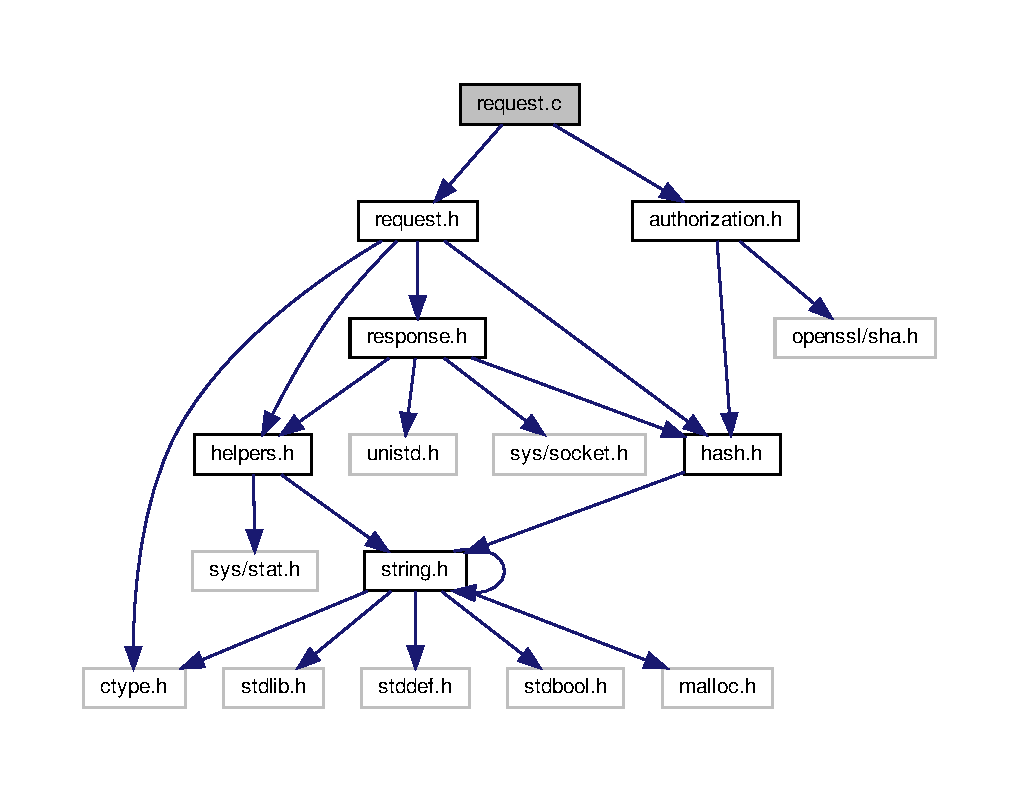
\includegraphics[width=350pt]{request_8c__incl}
\end{center}
\end{figure}
\subsection*{Macros}
\begin{DoxyCompactItemize}
\item 
\#define \hyperlink{request_8c_a625c76f362da15a712974d925f99229b}{P\+A\+T\+H\+\_\+\+C\+A\+P\+A\+C\+I\+TY}~2083
\item 
\#define \hyperlink{request_8c_a3e6fc1fdb6d81b13f26c16eb5efddf19}{P\+A\+T\+H\+\_\+\+C\+A\+P\+A\+C\+I\+T\+Y\+\_\+\+A\+B\+S\+O\+L\+U\+TE}~(\hyperlink{request_8c_a625c76f362da15a712974d925f99229b}{P\+A\+T\+H\+\_\+\+C\+A\+P\+A\+C\+I\+TY} + 200)
\end{DoxyCompactItemize}
\subsection*{Functions}
\begin{DoxyCompactItemize}
\item 
void \hyperlink{request_8c_a6ad9fb0bca4937f21fcc0035d185ee79}{free\+\_\+http\+\_\+request} (\hyperlink{request_8h_a756b7ee6cbac4fbbd1af5dff0bcdec31}{Http\+Request} $\ast$http\+Request)
\begin{DoxyCompactList}\small\item\em frees the Http\+Request-\/\+Struct \end{DoxyCompactList}\item 
\hyperlink{response_8h_ab894955de8b1913b4944567ee865ba21}{Http\+Response\+Code} \hyperlink{request_8c_ae72f3dc28e74d58dfed16ca668615a35}{validate\+\_\+resource} (\hyperlink{hash_8h_a58bb615f9115c5b9b1a49a64d3737edf}{Hash\+List} $\ast$fields, \hyperlink{string_8h_a3d2981d9da3e25dd89371059777fdd12}{string} $\ast$resource, \hyperlink{string_8h_a3d2981d9da3e25dd89371059777fdd12}{string} $\ast$$\ast$path)
\begin{DoxyCompactList}\small\item\em validates the requested resource Makes sure that the client is only able to access files within the Document\+Root and returns the right response code \end{DoxyCompactList}\item 
\hyperlink{response_8h_ab894955de8b1913b4944567ee865ba21}{Http\+Response\+Code} \hyperlink{request_8c_a7c0804b52ef0eca32dab11a0daa6acf4}{parse\+\_\+http\+\_\+request} (\hyperlink{string_8h_a3d2981d9da3e25dd89371059777fdd12}{string} $\ast$request, \hyperlink{request_8h_a756b7ee6cbac4fbbd1af5dff0bcdec31}{Http\+Request} $\ast$$\ast$http\+Request, \hyperlink{string_8h_a3d2981d9da3e25dd89371059777fdd12}{string} $\ast$$\ast$static\+Page)
\begin{DoxyCompactList}\small\item\em parses the received buffer, returns a response code and fills the http\+Request-\/\+Struct \end{DoxyCompactList}\item 
bool \hyperlink{request_8c_a30612b73b293afcce8c322bb7bd9672d}{fill\+\_\+request\+\_\+string} (\hyperlink{string_8h_a3d2981d9da3e25dd89371059777fdd12}{string} $\ast$str\+Request, char $\ast$buffer, size\+\_\+t buffer\+Size)
\begin{DoxyCompactList}\small\item\em checks if the request string contains a valid header end (\textquotesingle{}~\newline
~\newline
\textquotesingle{}) \end{DoxyCompactList}\end{DoxyCompactItemize}


\subsection{Macro Definition Documentation}
\mbox{\Hypertarget{request_8c_a625c76f362da15a712974d925f99229b}\label{request_8c_a625c76f362da15a712974d925f99229b}} 
\index{request.\+c@{request.\+c}!P\+A\+T\+H\+\_\+\+C\+A\+P\+A\+C\+I\+TY@{P\+A\+T\+H\+\_\+\+C\+A\+P\+A\+C\+I\+TY}}
\index{P\+A\+T\+H\+\_\+\+C\+A\+P\+A\+C\+I\+TY@{P\+A\+T\+H\+\_\+\+C\+A\+P\+A\+C\+I\+TY}!request.\+c@{request.\+c}}
\subsubsection{\texorpdfstring{P\+A\+T\+H\+\_\+\+C\+A\+P\+A\+C\+I\+TY}{PATH\_CAPACITY}}
{\footnotesize\ttfamily \#define P\+A\+T\+H\+\_\+\+C\+A\+P\+A\+C\+I\+TY~2083}

\mbox{\Hypertarget{request_8c_a3e6fc1fdb6d81b13f26c16eb5efddf19}\label{request_8c_a3e6fc1fdb6d81b13f26c16eb5efddf19}} 
\index{request.\+c@{request.\+c}!P\+A\+T\+H\+\_\+\+C\+A\+P\+A\+C\+I\+T\+Y\+\_\+\+A\+B\+S\+O\+L\+U\+TE@{P\+A\+T\+H\+\_\+\+C\+A\+P\+A\+C\+I\+T\+Y\+\_\+\+A\+B\+S\+O\+L\+U\+TE}}
\index{P\+A\+T\+H\+\_\+\+C\+A\+P\+A\+C\+I\+T\+Y\+\_\+\+A\+B\+S\+O\+L\+U\+TE@{P\+A\+T\+H\+\_\+\+C\+A\+P\+A\+C\+I\+T\+Y\+\_\+\+A\+B\+S\+O\+L\+U\+TE}!request.\+c@{request.\+c}}
\subsubsection{\texorpdfstring{P\+A\+T\+H\+\_\+\+C\+A\+P\+A\+C\+I\+T\+Y\+\_\+\+A\+B\+S\+O\+L\+U\+TE}{PATH\_CAPACITY\_ABSOLUTE}}
{\footnotesize\ttfamily \#define P\+A\+T\+H\+\_\+\+C\+A\+P\+A\+C\+I\+T\+Y\+\_\+\+A\+B\+S\+O\+L\+U\+TE~(\hyperlink{request_8c_a625c76f362da15a712974d925f99229b}{P\+A\+T\+H\+\_\+\+C\+A\+P\+A\+C\+I\+TY} + 200)}



\subsection{Function Documentation}
\mbox{\Hypertarget{request_8c_a30612b73b293afcce8c322bb7bd9672d}\label{request_8c_a30612b73b293afcce8c322bb7bd9672d}} 
\index{request.\+c@{request.\+c}!fill\+\_\+request\+\_\+string@{fill\+\_\+request\+\_\+string}}
\index{fill\+\_\+request\+\_\+string@{fill\+\_\+request\+\_\+string}!request.\+c@{request.\+c}}
\subsubsection{\texorpdfstring{fill\+\_\+request\+\_\+string()}{fill\_request\_string()}}
{\footnotesize\ttfamily bool fill\+\_\+request\+\_\+string (\begin{DoxyParamCaption}\item[{\hyperlink{string_8h_a3d2981d9da3e25dd89371059777fdd12}{string} $\ast$}]{str\+Request,  }\item[{char $\ast$}]{buffer,  }\item[{size\+\_\+t}]{buffer\+Size }\end{DoxyParamCaption})}



checks if the request string contains a valid header end (\textquotesingle{}~\newline
~\newline
\textquotesingle{}) 


\begin{DoxyParams}{Parameters}
{\em str\+Request} & the whole request as string \\
\hline
{\em buffer} & the current buffer data \\
\hline
{\em buffer\+Size} & the current buffer data size \\
\hline
\end{DoxyParams}
\begin{DoxyReturn}{Returns}
true if end of header was found, otherwise false 
\end{DoxyReturn}
\mbox{\Hypertarget{request_8c_a6ad9fb0bca4937f21fcc0035d185ee79}\label{request_8c_a6ad9fb0bca4937f21fcc0035d185ee79}} 
\index{request.\+c@{request.\+c}!free\+\_\+http\+\_\+request@{free\+\_\+http\+\_\+request}}
\index{free\+\_\+http\+\_\+request@{free\+\_\+http\+\_\+request}!request.\+c@{request.\+c}}
\subsubsection{\texorpdfstring{free\+\_\+http\+\_\+request()}{free\_http\_request()}}
{\footnotesize\ttfamily void free\+\_\+http\+\_\+request (\begin{DoxyParamCaption}\item[{\hyperlink{request_8h_a756b7ee6cbac4fbbd1af5dff0bcdec31}{Http\+Request} $\ast$}]{http\+Request }\end{DoxyParamCaption})}



frees the Http\+Request-\/\+Struct 

\begin{DoxyAuthor}{Author}
Marcel Weski 
\end{DoxyAuthor}

\begin{DoxyParams}{Parameters}
{\em http\+Request} & struct to free \\
\hline
\end{DoxyParams}
\mbox{\Hypertarget{request_8c_a7c0804b52ef0eca32dab11a0daa6acf4}\label{request_8c_a7c0804b52ef0eca32dab11a0daa6acf4}} 
\index{request.\+c@{request.\+c}!parse\+\_\+http\+\_\+request@{parse\+\_\+http\+\_\+request}}
\index{parse\+\_\+http\+\_\+request@{parse\+\_\+http\+\_\+request}!request.\+c@{request.\+c}}
\subsubsection{\texorpdfstring{parse\+\_\+http\+\_\+request()}{parse\_http\_request()}}
{\footnotesize\ttfamily \hyperlink{response_8h_ab894955de8b1913b4944567ee865ba21}{Http\+Response\+Code} parse\+\_\+http\+\_\+request (\begin{DoxyParamCaption}\item[{\hyperlink{string_8h_a3d2981d9da3e25dd89371059777fdd12}{string} $\ast$}]{request,  }\item[{\hyperlink{request_8h_a756b7ee6cbac4fbbd1af5dff0bcdec31}{Http\+Request} $\ast$$\ast$}]{http\+Request,  }\item[{\hyperlink{string_8h_a3d2981d9da3e25dd89371059777fdd12}{string} $\ast$$\ast$}]{static\+Page }\end{DoxyParamCaption})}



parses the received buffer, returns a response code and fills the http\+Request-\/\+Struct 

\begin{DoxyAuthor}{Author}
Marcel Weski 
\end{DoxyAuthor}

\begin{DoxyParams}{Parameters}
{\em request} & string of buffers \\
\hline
{\em http\+Request} & the filled http\+Request. Must be freed! \\
\hline
{\em static\+Page} & returns the debug-\/\+Page if /debug is requested. Must be freed! \\
\hline
\end{DoxyParams}
\begin{DoxyReturn}{Returns}
int the response code 
\end{DoxyReturn}
\mbox{\Hypertarget{request_8c_ae72f3dc28e74d58dfed16ca668615a35}\label{request_8c_ae72f3dc28e74d58dfed16ca668615a35}} 
\index{request.\+c@{request.\+c}!validate\+\_\+resource@{validate\+\_\+resource}}
\index{validate\+\_\+resource@{validate\+\_\+resource}!request.\+c@{request.\+c}}
\subsubsection{\texorpdfstring{validate\+\_\+resource()}{validate\_resource()}}
{\footnotesize\ttfamily \hyperlink{response_8h_ab894955de8b1913b4944567ee865ba21}{Http\+Response\+Code} validate\+\_\+resource (\begin{DoxyParamCaption}\item[{\hyperlink{hash_8h_a58bb615f9115c5b9b1a49a64d3737edf}{Hash\+List} $\ast$}]{hash\+List,  }\item[{\hyperlink{string_8h_a3d2981d9da3e25dd89371059777fdd12}{string} $\ast$}]{resource,  }\item[{\hyperlink{string_8h_a3d2981d9da3e25dd89371059777fdd12}{string} $\ast$$\ast$}]{path }\end{DoxyParamCaption})}



validates the requested resource Makes sure that the client is only able to access files within the Document\+Root and returns the right response code 

\begin{DoxyAuthor}{Author}
Marcel Weski 
\end{DoxyAuthor}

\begin{DoxyParams}{Parameters}
{\em hash\+List} & fields of the request \\
\hline
{\em resource} & requested resource \\
\hline
{\em path} & the new absolute path from the resource, if the file exists. Must be freed! \\
\hline
\end{DoxyParams}
\begin{DoxyReturn}{Returns}
200, if the file exists. 403, if the access is not allowed (specific files and all files outside the document root). 404, if the file doesn\textquotesingle{}t exists 
\end{DoxyReturn}

\hypertarget{request_8h}{}\section{request.\+h File Reference}
\label{request_8h}\index{request.\+h@{request.\+h}}
{\ttfamily \#include $<$ctype.\+h$>$}\newline
{\ttfamily \#include \char`\"{}hash.\+h\char`\"{}}\newline
{\ttfamily \#include \char`\"{}response.\+h\char`\"{}}\newline
{\ttfamily \#include \char`\"{}helpers.\+h\char`\"{}}\newline
Include dependency graph for request.\+h\+:
\nopagebreak
\begin{figure}[H]
\begin{center}
\leavevmode
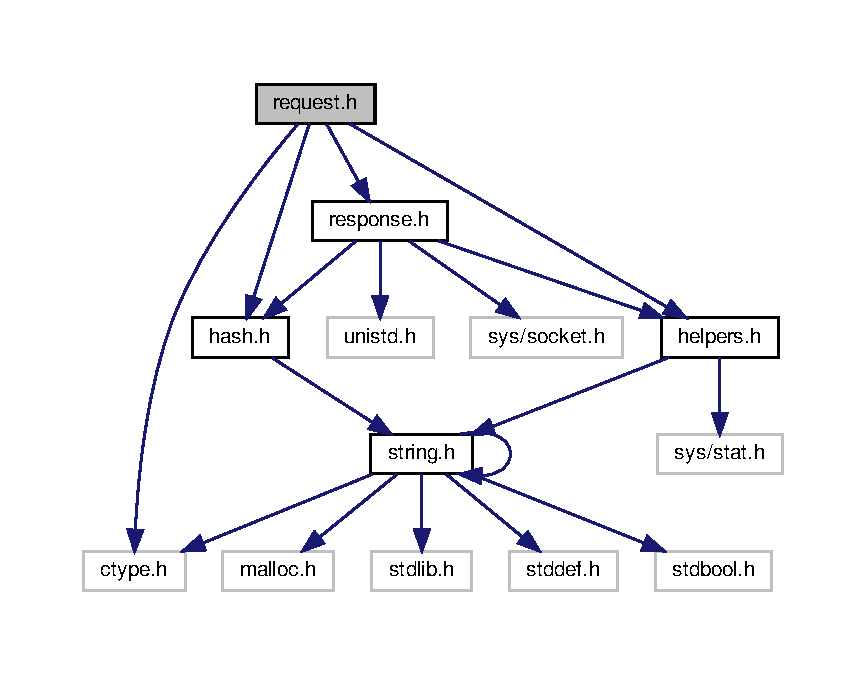
\includegraphics[width=350pt]{request_8h__incl}
\end{center}
\end{figure}
This graph shows which files directly or indirectly include this file\+:
\nopagebreak
\begin{figure}[H]
\begin{center}
\leavevmode
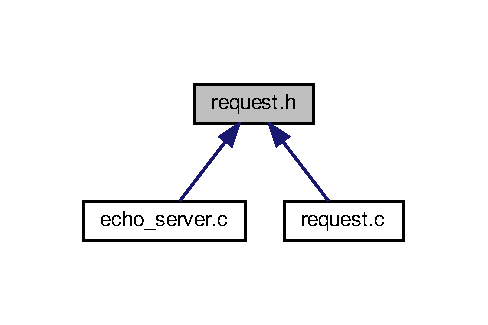
\includegraphics[width=234pt]{request_8h__dep__incl}
\end{center}
\end{figure}
\subsection*{Data Structures}
\begin{DoxyCompactItemize}
\item 
struct \hyperlink{structhttp__request__struct}{http\+\_\+request\+\_\+struct}
\end{DoxyCompactItemize}
\subsection*{Typedefs}
\begin{DoxyCompactItemize}
\item 
typedef struct \hyperlink{structhttp__request__struct}{http\+\_\+request\+\_\+struct} \hyperlink{request_8h_a756b7ee6cbac4fbbd1af5dff0bcdec31}{Http\+Request}
\end{DoxyCompactItemize}
\subsection*{Functions}
\begin{DoxyCompactItemize}
\item 
void \hyperlink{request_8h_a6ad9fb0bca4937f21fcc0035d185ee79}{free\+\_\+http\+\_\+request} (\hyperlink{request_8h_a756b7ee6cbac4fbbd1af5dff0bcdec31}{Http\+Request} $\ast$http\+Request)
\begin{DoxyCompactList}\small\item\em frees the Http\+Request-\/\+Struct \end{DoxyCompactList}\item 
\hyperlink{response_8h_ab894955de8b1913b4944567ee865ba21}{Http\+Response\+Code} \hyperlink{request_8h_acd6c0e6599db94c90692a4b94c244a71}{validate\+\_\+resource} (\hyperlink{hash_8h_a58bb615f9115c5b9b1a49a64d3737edf}{Hash\+List} $\ast$hash\+List, \hyperlink{string_8h_a3d2981d9da3e25dd89371059777fdd12}{string} $\ast$resource, \hyperlink{string_8h_a3d2981d9da3e25dd89371059777fdd12}{string} $\ast$$\ast$path)
\begin{DoxyCompactList}\small\item\em validates the requested resource Makes sure that the client is only able to access files within the Document\+Root and returns the right response code \end{DoxyCompactList}\item 
\hyperlink{response_8h_ab894955de8b1913b4944567ee865ba21}{Http\+Response\+Code} \hyperlink{request_8h_a7c0804b52ef0eca32dab11a0daa6acf4}{parse\+\_\+http\+\_\+request} (\hyperlink{string_8h_a3d2981d9da3e25dd89371059777fdd12}{string} $\ast$request, \hyperlink{request_8h_a756b7ee6cbac4fbbd1af5dff0bcdec31}{Http\+Request} $\ast$$\ast$http\+Request, \hyperlink{string_8h_a3d2981d9da3e25dd89371059777fdd12}{string} $\ast$$\ast$static\+Page)
\begin{DoxyCompactList}\small\item\em parses the received buffer, returns a response code and fills the http\+Request-\/\+Struct \end{DoxyCompactList}\item 
bool \hyperlink{request_8h_a30612b73b293afcce8c322bb7bd9672d}{fill\+\_\+request\+\_\+string} (\hyperlink{string_8h_a3d2981d9da3e25dd89371059777fdd12}{string} $\ast$str\+Request, char $\ast$buffer, size\+\_\+t buffer\+Size)
\begin{DoxyCompactList}\small\item\em checks if the request string contains a valid header end (\textquotesingle{}~\newline
~\newline
\textquotesingle{}) \end{DoxyCompactList}\end{DoxyCompactItemize}


\subsection{Detailed Description}
\begin{DoxyAuthor}{Author}
Marcel Weski 
\end{DoxyAuthor}


\subsection{Typedef Documentation}
\mbox{\Hypertarget{request_8h_a756b7ee6cbac4fbbd1af5dff0bcdec31}\label{request_8h_a756b7ee6cbac4fbbd1af5dff0bcdec31}} 
\index{request.\+h@{request.\+h}!Http\+Request@{Http\+Request}}
\index{Http\+Request@{Http\+Request}!request.\+h@{request.\+h}}
\subsubsection{\texorpdfstring{Http\+Request}{HttpRequest}}
{\footnotesize\ttfamily typedef struct \hyperlink{structhttp__request__struct}{http\+\_\+request\+\_\+struct}  \hyperlink{request_8h_a756b7ee6cbac4fbbd1af5dff0bcdec31}{Http\+Request}}



\subsection{Function Documentation}
\mbox{\Hypertarget{request_8h_a30612b73b293afcce8c322bb7bd9672d}\label{request_8h_a30612b73b293afcce8c322bb7bd9672d}} 
\index{request.\+h@{request.\+h}!fill\+\_\+request\+\_\+string@{fill\+\_\+request\+\_\+string}}
\index{fill\+\_\+request\+\_\+string@{fill\+\_\+request\+\_\+string}!request.\+h@{request.\+h}}
\subsubsection{\texorpdfstring{fill\+\_\+request\+\_\+string()}{fill\_request\_string()}}
{\footnotesize\ttfamily bool fill\+\_\+request\+\_\+string (\begin{DoxyParamCaption}\item[{\hyperlink{string_8h_a3d2981d9da3e25dd89371059777fdd12}{string} $\ast$}]{str\+Request,  }\item[{char $\ast$}]{buffer,  }\item[{size\+\_\+t}]{buffer\+Size }\end{DoxyParamCaption})}



checks if the request string contains a valid header end (\textquotesingle{}~\newline
~\newline
\textquotesingle{}) 


\begin{DoxyParams}{Parameters}
{\em str\+Request} & the whole request as string \\
\hline
{\em buffer} & the current buffer data \\
\hline
{\em buffer\+Size} & the current buffer data size \\
\hline
\end{DoxyParams}
\begin{DoxyReturn}{Returns}
true if end of header was found, otherwise false 
\end{DoxyReturn}
\mbox{\Hypertarget{request_8h_a6ad9fb0bca4937f21fcc0035d185ee79}\label{request_8h_a6ad9fb0bca4937f21fcc0035d185ee79}} 
\index{request.\+h@{request.\+h}!free\+\_\+http\+\_\+request@{free\+\_\+http\+\_\+request}}
\index{free\+\_\+http\+\_\+request@{free\+\_\+http\+\_\+request}!request.\+h@{request.\+h}}
\subsubsection{\texorpdfstring{free\+\_\+http\+\_\+request()}{free\_http\_request()}}
{\footnotesize\ttfamily void free\+\_\+http\+\_\+request (\begin{DoxyParamCaption}\item[{\hyperlink{request_8h_a756b7ee6cbac4fbbd1af5dff0bcdec31}{Http\+Request} $\ast$}]{http\+Request }\end{DoxyParamCaption})}



frees the Http\+Request-\/\+Struct 

\begin{DoxyAuthor}{Author}
Marcel Weski 
\end{DoxyAuthor}

\begin{DoxyParams}{Parameters}
{\em http\+Request} & struct to free \\
\hline
\end{DoxyParams}
\mbox{\Hypertarget{request_8h_a7c0804b52ef0eca32dab11a0daa6acf4}\label{request_8h_a7c0804b52ef0eca32dab11a0daa6acf4}} 
\index{request.\+h@{request.\+h}!parse\+\_\+http\+\_\+request@{parse\+\_\+http\+\_\+request}}
\index{parse\+\_\+http\+\_\+request@{parse\+\_\+http\+\_\+request}!request.\+h@{request.\+h}}
\subsubsection{\texorpdfstring{parse\+\_\+http\+\_\+request()}{parse\_http\_request()}}
{\footnotesize\ttfamily \hyperlink{response_8h_ab894955de8b1913b4944567ee865ba21}{Http\+Response\+Code} parse\+\_\+http\+\_\+request (\begin{DoxyParamCaption}\item[{\hyperlink{string_8h_a3d2981d9da3e25dd89371059777fdd12}{string} $\ast$}]{request,  }\item[{\hyperlink{request_8h_a756b7ee6cbac4fbbd1af5dff0bcdec31}{Http\+Request} $\ast$$\ast$}]{http\+Request,  }\item[{\hyperlink{string_8h_a3d2981d9da3e25dd89371059777fdd12}{string} $\ast$$\ast$}]{static\+Page }\end{DoxyParamCaption})}



parses the received buffer, returns a response code and fills the http\+Request-\/\+Struct 

\begin{DoxyAuthor}{Author}
Marcel Weski 
\end{DoxyAuthor}

\begin{DoxyParams}{Parameters}
{\em request} & string of buffers \\
\hline
{\em http\+Request} & the filled http\+Request. Must be freed! \\
\hline
{\em static\+Page} & returns the debug-\/\+Page if /debug is requested. Must be freed! \\
\hline
\end{DoxyParams}
\begin{DoxyReturn}{Returns}
int the response code 
\end{DoxyReturn}
\mbox{\Hypertarget{request_8h_acd6c0e6599db94c90692a4b94c244a71}\label{request_8h_acd6c0e6599db94c90692a4b94c244a71}} 
\index{request.\+h@{request.\+h}!validate\+\_\+resource@{validate\+\_\+resource}}
\index{validate\+\_\+resource@{validate\+\_\+resource}!request.\+h@{request.\+h}}
\subsubsection{\texorpdfstring{validate\+\_\+resource()}{validate\_resource()}}
{\footnotesize\ttfamily \hyperlink{response_8h_ab894955de8b1913b4944567ee865ba21}{Http\+Response\+Code} validate\+\_\+resource (\begin{DoxyParamCaption}\item[{\hyperlink{hash_8h_a58bb615f9115c5b9b1a49a64d3737edf}{Hash\+List} $\ast$}]{hash\+List,  }\item[{\hyperlink{string_8h_a3d2981d9da3e25dd89371059777fdd12}{string} $\ast$}]{resource,  }\item[{\hyperlink{string_8h_a3d2981d9da3e25dd89371059777fdd12}{string} $\ast$$\ast$}]{path }\end{DoxyParamCaption})}



validates the requested resource Makes sure that the client is only able to access files within the Document\+Root and returns the right response code 

\begin{DoxyAuthor}{Author}
Marcel Weski 
\end{DoxyAuthor}

\begin{DoxyParams}{Parameters}
{\em hash\+List} & fields of the request \\
\hline
{\em resource} & requested resource \\
\hline
{\em path} & the new absolute path from the resource, if the file exists. Must be freed! \\
\hline
\end{DoxyParams}
\begin{DoxyReturn}{Returns}
200, if the file exists. 403, if the access is not allowed (specific files and all files outside the document root). 404, if the file doesn\textquotesingle{}t exists 
\end{DoxyReturn}

\hypertarget{response_8c}{}\section{response.\+c File Reference}
\label{response_8c}\index{response.\+c@{response.\+c}}
{\ttfamily \#include \char`\"{}response.\+h\char`\"{}}\newline
{\ttfamily \#include \char`\"{}authorization.\+h\char`\"{}}\newline
Include dependency graph for response.\+c\+:
\nopagebreak
\begin{figure}[H]
\begin{center}
\leavevmode
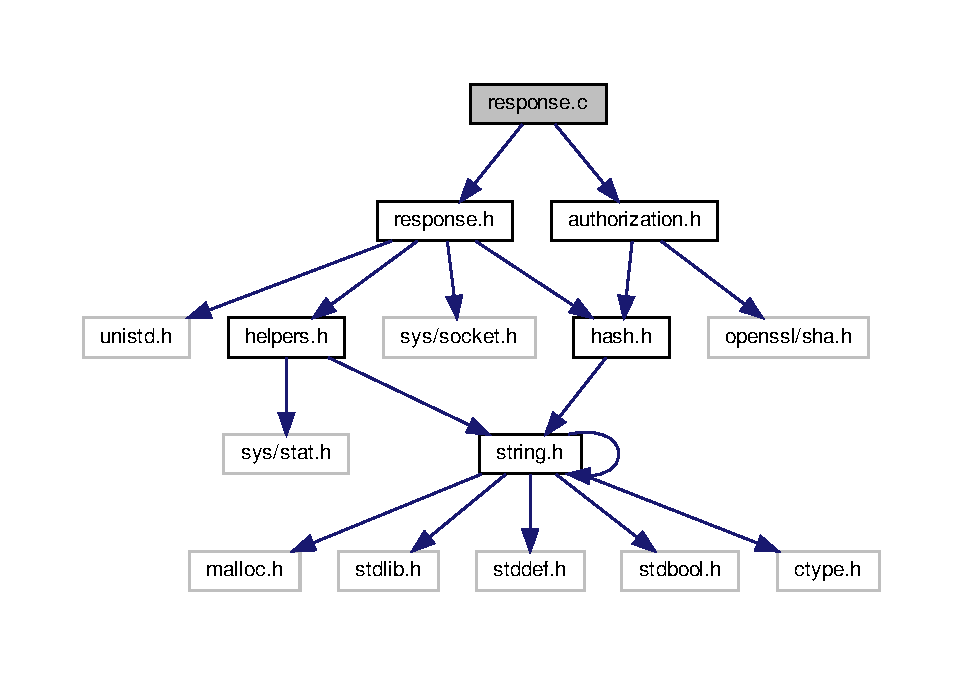
\includegraphics[width=350pt]{response_8c__incl}
\end{center}
\end{figure}
\subsection*{Macros}
\begin{DoxyCompactItemize}
\item 
\#define \hyperlink{response_8c_af00aa3c79fe31d435739c34e4c989835}{S\+E\+R\+V\+E\+R\+\_\+\+N\+A\+ME}~\char`\"{}P\+SE H\+T\+TP-\/Server v1.\+0\char`\"{}
\item 
\#define \hyperlink{response_8c_a09dbbd73a84cf772b421c6024b65b1fd}{F\+I\+L\+E\+\_\+\+B\+U\+F\+F\+E\+R\+\_\+\+S\+I\+ZE}~65536
\end{DoxyCompactItemize}
\subsection*{Functions}
\begin{DoxyCompactItemize}
\item 
char $\ast$ \hyperlink{response_8c_a3a784abd945fb5260d50fc0f6f46b595}{code\+\_\+to\+\_\+string} (\hyperlink{response_8h_ab894955de8b1913b4944567ee865ba21}{Http\+Response\+Code} code)
\begin{DoxyCompactList}\small\item\em converts the responsecode to a string \end{DoxyCompactList}\item 
\hyperlink{string_8h_a3d2981d9da3e25dd89371059777fdd12}{string} $\ast$ \hyperlink{response_8c_a7066937e68de3b306d0fc62ca661ef10}{build\+\_\+http\+\_\+response\+\_\+header} (\hyperlink{response_8h_ab894955de8b1913b4944567ee865ba21}{Http\+Response\+Code} code, \hyperlink{hash_8h_a58bb615f9115c5b9b1a49a64d3737edf}{Hash\+List} $\ast$fields)
\begin{DoxyCompactList}\small\item\em simple wrapper to build H\+T\+TP response \end{DoxyCompactList}\item 
void \hyperlink{response_8c_a1acb37e021e566b839a0f74fc57961a9}{send\+\_\+http\+\_\+response} (int target\+Stream, \hyperlink{response_8h_ab894955de8b1913b4944567ee865ba21}{Http\+Response\+Code} code, \hyperlink{string_8h_a3d2981d9da3e25dd89371059777fdd12}{string} $\ast$path, \hyperlink{string_8h_a3d2981d9da3e25dd89371059777fdd12}{string} $\ast$static\+Page)
\begin{DoxyCompactList}\small\item\em uses the build\+\_\+http\+\_\+response\+\_\+header function to send a response to the client \end{DoxyCompactList}\end{DoxyCompactItemize}


\subsection{Macro Definition Documentation}
\mbox{\Hypertarget{response_8c_a09dbbd73a84cf772b421c6024b65b1fd}\label{response_8c_a09dbbd73a84cf772b421c6024b65b1fd}} 
\index{response.\+c@{response.\+c}!F\+I\+L\+E\+\_\+\+B\+U\+F\+F\+E\+R\+\_\+\+S\+I\+ZE@{F\+I\+L\+E\+\_\+\+B\+U\+F\+F\+E\+R\+\_\+\+S\+I\+ZE}}
\index{F\+I\+L\+E\+\_\+\+B\+U\+F\+F\+E\+R\+\_\+\+S\+I\+ZE@{F\+I\+L\+E\+\_\+\+B\+U\+F\+F\+E\+R\+\_\+\+S\+I\+ZE}!response.\+c@{response.\+c}}
\subsubsection{\texorpdfstring{F\+I\+L\+E\+\_\+\+B\+U\+F\+F\+E\+R\+\_\+\+S\+I\+ZE}{FILE\_BUFFER\_SIZE}}
{\footnotesize\ttfamily \#define F\+I\+L\+E\+\_\+\+B\+U\+F\+F\+E\+R\+\_\+\+S\+I\+ZE~65536}

\mbox{\Hypertarget{response_8c_af00aa3c79fe31d435739c34e4c989835}\label{response_8c_af00aa3c79fe31d435739c34e4c989835}} 
\index{response.\+c@{response.\+c}!S\+E\+R\+V\+E\+R\+\_\+\+N\+A\+ME@{S\+E\+R\+V\+E\+R\+\_\+\+N\+A\+ME}}
\index{S\+E\+R\+V\+E\+R\+\_\+\+N\+A\+ME@{S\+E\+R\+V\+E\+R\+\_\+\+N\+A\+ME}!response.\+c@{response.\+c}}
\subsubsection{\texorpdfstring{S\+E\+R\+V\+E\+R\+\_\+\+N\+A\+ME}{SERVER\_NAME}}
{\footnotesize\ttfamily \#define S\+E\+R\+V\+E\+R\+\_\+\+N\+A\+ME~\char`\"{}P\+SE H\+T\+TP-\/Server v1.\+0\char`\"{}}



\subsection{Function Documentation}
\mbox{\Hypertarget{response_8c_a7066937e68de3b306d0fc62ca661ef10}\label{response_8c_a7066937e68de3b306d0fc62ca661ef10}} 
\index{response.\+c@{response.\+c}!build\+\_\+http\+\_\+response\+\_\+header@{build\+\_\+http\+\_\+response\+\_\+header}}
\index{build\+\_\+http\+\_\+response\+\_\+header@{build\+\_\+http\+\_\+response\+\_\+header}!response.\+c@{response.\+c}}
\subsubsection{\texorpdfstring{build\+\_\+http\+\_\+response\+\_\+header()}{build\_http\_response\_header()}}
{\footnotesize\ttfamily \hyperlink{string_8h_a3d2981d9da3e25dd89371059777fdd12}{string}$\ast$ build\+\_\+http\+\_\+response\+\_\+header (\begin{DoxyParamCaption}\item[{\hyperlink{response_8h_ab894955de8b1913b4944567ee865ba21}{Http\+Response\+Code}}]{code,  }\item[{\hyperlink{hash_8h_a58bb615f9115c5b9b1a49a64d3737edf}{Hash\+List} $\ast$}]{fields }\end{DoxyParamCaption})}



simple wrapper to build H\+T\+TP response 

Please ensure your Hashes are used the following way\+: key -\/$>$ field name value -\/$>$ field value the function will add the \textquotesingle{}\+:\textquotesingle{} separator after the name itself.

the fuction will return N\+U\+LL on failure

\begin{DoxyAuthor}{Author}
Björn Marx
\end{DoxyAuthor}

\begin{DoxyParams}{Parameters}
{\em code} & desired H\+T\+TP response code, chosen from Http\+Response\+Codes enum \\
\hline
{\em fields} & list of header fields \\
\hline
\end{DoxyParams}
\begin{DoxyReturn}{Returns}
Http response as string 
\end{DoxyReturn}
\mbox{\Hypertarget{response_8c_a3a784abd945fb5260d50fc0f6f46b595}\label{response_8c_a3a784abd945fb5260d50fc0f6f46b595}} 
\index{response.\+c@{response.\+c}!code\+\_\+to\+\_\+string@{code\+\_\+to\+\_\+string}}
\index{code\+\_\+to\+\_\+string@{code\+\_\+to\+\_\+string}!response.\+c@{response.\+c}}
\subsubsection{\texorpdfstring{code\+\_\+to\+\_\+string()}{code\_to\_string()}}
{\footnotesize\ttfamily char$\ast$ code\+\_\+to\+\_\+string (\begin{DoxyParamCaption}\item[{\hyperlink{response_8h_ab894955de8b1913b4944567ee865ba21}{Http\+Response\+Code}}]{code }\end{DoxyParamCaption})}



converts the responsecode to a string 

\begin{DoxyAuthor}{Author}
Björn Marx
\end{DoxyAuthor}
\begin{DoxyReturn}{Returns}
code as string 
\end{DoxyReturn}
\mbox{\Hypertarget{response_8c_a1acb37e021e566b839a0f74fc57961a9}\label{response_8c_a1acb37e021e566b839a0f74fc57961a9}} 
\index{response.\+c@{response.\+c}!send\+\_\+http\+\_\+response@{send\+\_\+http\+\_\+response}}
\index{send\+\_\+http\+\_\+response@{send\+\_\+http\+\_\+response}!response.\+c@{response.\+c}}
\subsubsection{\texorpdfstring{send\+\_\+http\+\_\+response()}{send\_http\_response()}}
{\footnotesize\ttfamily void send\+\_\+http\+\_\+response (\begin{DoxyParamCaption}\item[{int}]{target\+Stream,  }\item[{\hyperlink{response_8h_ab894955de8b1913b4944567ee865ba21}{Http\+Response\+Code}}]{code,  }\item[{\hyperlink{string_8h_a3d2981d9da3e25dd89371059777fdd12}{string} $\ast$}]{path,  }\item[{\hyperlink{string_8h_a3d2981d9da3e25dd89371059777fdd12}{string} $\ast$}]{static\+Page }\end{DoxyParamCaption})}



uses the build\+\_\+http\+\_\+response\+\_\+header function to send a response to the client 

\begin{DoxyAuthor}{Author}
Marcel Weski 
\end{DoxyAuthor}

\begin{DoxyParams}{Parameters}
{\em target\+Stream} & socket or stdout stream \\
\hline
{\em code} & response\+Code returned by the parse\+\_\+http\+\_\+request function \\
\hline
{\em path} & requested absolute file path \\
\hline
{\em static\+Page} & contains a string if /debug was requested \\
\hline
\end{DoxyParams}

\hypertarget{response_8h}{}\section{response.\+h File Reference}
\label{response_8h}\index{response.\+h@{response.\+h}}
{\ttfamily \#include $<$unistd.\+h$>$}\newline
{\ttfamily \#include $<$sys/socket.\+h$>$}\newline
{\ttfamily \#include \char`\"{}hash.\+h\char`\"{}}\newline
{\ttfamily \#include \char`\"{}helpers.\+h\char`\"{}}\newline
Include dependency graph for response.\+h\+:
\nopagebreak
\begin{figure}[H]
\begin{center}
\leavevmode
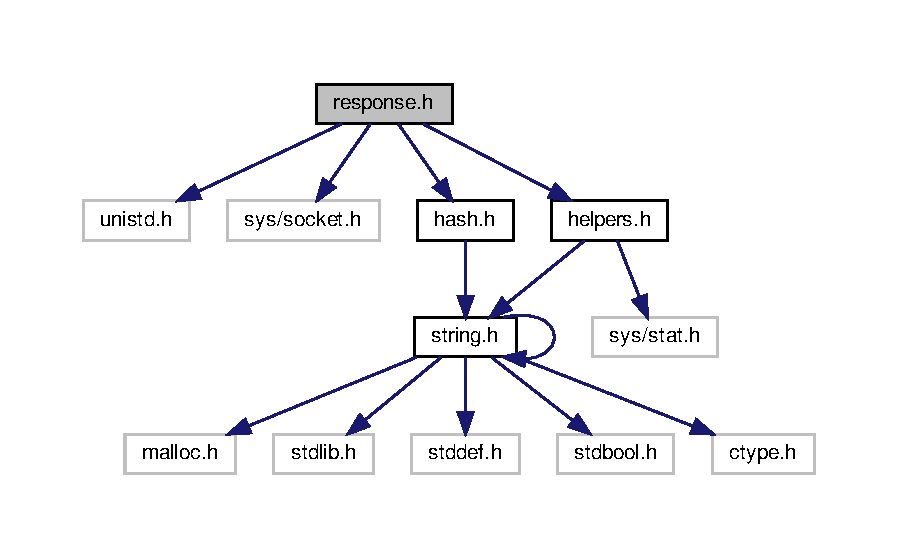
\includegraphics[width=350pt]{response_8h__incl}
\end{center}
\end{figure}
This graph shows which files directly or indirectly include this file\+:
\nopagebreak
\begin{figure}[H]
\begin{center}
\leavevmode
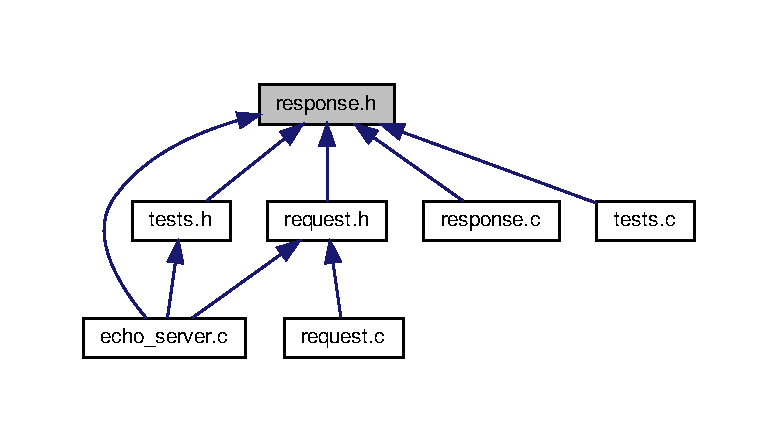
\includegraphics[width=350pt]{response_8h__dep__incl}
\end{center}
\end{figure}
\subsection*{Enumerations}
\begin{DoxyCompactItemize}
\item 
enum \hyperlink{response_8h_ab894955de8b1913b4944567ee865ba21}{Http\+Response\+Code} \{ \newline
\hyperlink{response_8h_ab894955de8b1913b4944567ee865ba21a2bc49ec37d6a5715dd23e85f1ff5bb59}{OK} = 200, 
\hyperlink{response_8h_ab894955de8b1913b4944567ee865ba21aef4e18cf5dacaf9d0cb90c72663a1b60}{B\+A\+D\+\_\+\+R\+E\+Q\+U\+E\+ST} = 400, 
\hyperlink{response_8h_ab894955de8b1913b4944567ee865ba21aca808e0004f9d8808506cf69bd4a224c}{U\+N\+A\+U\+T\+H\+O\+R\+I\+Z\+ED} = 401, 
\hyperlink{response_8h_ab894955de8b1913b4944567ee865ba21a4b4068e636cd02a6e87e8d3920383d67}{F\+O\+R\+B\+I\+D\+D\+EN} = 403, 
\newline
\hyperlink{response_8h_ab894955de8b1913b4944567ee865ba21acdaa2919bac56fe1090eb3dbb9526472}{N\+O\+T\+\_\+\+F\+O\+U\+ND} = 404, 
\hyperlink{response_8h_ab894955de8b1913b4944567ee865ba21a5bc385218b6fd9392f95cfc35e20effe}{M\+E\+T\+H\+O\+D\+\_\+\+N\+O\+T\+\_\+\+A\+L\+L\+O\+W\+ED} = 405, 
\hyperlink{response_8h_ab894955de8b1913b4944567ee865ba21a12bcc9d9958a22b983e65f77f3faf90b}{N\+O\+T\+\_\+\+I\+M\+P\+L\+E\+M\+E\+N\+T\+ED} = 501, 
\hyperlink{response_8h_ab894955de8b1913b4944567ee865ba21a803023bc4cc6926389c140ec20c77dd0}{V\+E\+R\+S\+I\+O\+N\+\_\+\+N\+O\+T\+\_\+\+S\+U\+P\+P\+O\+R\+T\+ED} = 505
 \}\begin{DoxyCompactList}\small\item\em struct defining supported H\+T\+TP response codes \end{DoxyCompactList}
\end{DoxyCompactItemize}
\subsection*{Functions}
\begin{DoxyCompactItemize}
\item 
char $\ast$ \hyperlink{response_8h_a3a784abd945fb5260d50fc0f6f46b595}{code\+\_\+to\+\_\+string} (\hyperlink{response_8h_ab894955de8b1913b4944567ee865ba21}{Http\+Response\+Code} code)
\begin{DoxyCompactList}\small\item\em converts the responsecode to a string \end{DoxyCompactList}\item 
\hyperlink{string_8h_a3d2981d9da3e25dd89371059777fdd12}{string} $\ast$ \hyperlink{response_8h_a7066937e68de3b306d0fc62ca661ef10}{build\+\_\+http\+\_\+response\+\_\+header} (\hyperlink{response_8h_ab894955de8b1913b4944567ee865ba21}{Http\+Response\+Code} code, \hyperlink{hash_8h_a58bb615f9115c5b9b1a49a64d3737edf}{Hash\+List} $\ast$fields)
\begin{DoxyCompactList}\small\item\em simple wrapper to build H\+T\+TP response \end{DoxyCompactList}\item 
void \hyperlink{response_8h_a1acb37e021e566b839a0f74fc57961a9}{send\+\_\+http\+\_\+response} (int target\+Stream, \hyperlink{response_8h_ab894955de8b1913b4944567ee865ba21}{Http\+Response\+Code} code, \hyperlink{string_8h_a3d2981d9da3e25dd89371059777fdd12}{string} $\ast$path, \hyperlink{string_8h_a3d2981d9da3e25dd89371059777fdd12}{string} $\ast$static\+Page)
\begin{DoxyCompactList}\small\item\em uses the build\+\_\+http\+\_\+response\+\_\+header function to send a response to the client \end{DoxyCompactList}\end{DoxyCompactItemize}


\subsection{Detailed Description}
\begin{DoxyAuthor}{Author}
Björn Marx 

Marcel Weski 
\end{DoxyAuthor}
\begin{DoxyDate}{Date}
26/04/19 
\end{DoxyDate}


\subsection{Enumeration Type Documentation}
\mbox{\Hypertarget{response_8h_ab894955de8b1913b4944567ee865ba21}\label{response_8h_ab894955de8b1913b4944567ee865ba21}} 
\index{response.\+h@{response.\+h}!Http\+Response\+Code@{Http\+Response\+Code}}
\index{Http\+Response\+Code@{Http\+Response\+Code}!response.\+h@{response.\+h}}
\subsubsection{\texorpdfstring{Http\+Response\+Code}{HttpResponseCode}}
{\footnotesize\ttfamily enum \hyperlink{response_8h_ab894955de8b1913b4944567ee865ba21}{Http\+Response\+Code}}



struct defining supported H\+T\+TP response codes 

\begin{DoxyAuthor}{Author}
Björn Marx 
\end{DoxyAuthor}
\begin{DoxyEnumFields}{Enumerator}
\raisebox{\heightof{T}}[0pt][0pt]{\index{OK@{OK}!response.\+h@{response.\+h}}\index{response.\+h@{response.\+h}!OK@{OK}}}\mbox{\Hypertarget{response_8h_ab894955de8b1913b4944567ee865ba21a2bc49ec37d6a5715dd23e85f1ff5bb59}\label{response_8h_ab894955de8b1913b4944567ee865ba21a2bc49ec37d6a5715dd23e85f1ff5bb59}} 
OK&\\
\hline

\raisebox{\heightof{T}}[0pt][0pt]{\index{B\+A\+D\+\_\+\+R\+E\+Q\+U\+E\+ST@{B\+A\+D\+\_\+\+R\+E\+Q\+U\+E\+ST}!response.\+h@{response.\+h}}\index{response.\+h@{response.\+h}!B\+A\+D\+\_\+\+R\+E\+Q\+U\+E\+ST@{B\+A\+D\+\_\+\+R\+E\+Q\+U\+E\+ST}}}\mbox{\Hypertarget{response_8h_ab894955de8b1913b4944567ee865ba21aef4e18cf5dacaf9d0cb90c72663a1b60}\label{response_8h_ab894955de8b1913b4944567ee865ba21aef4e18cf5dacaf9d0cb90c72663a1b60}} 
B\+A\+D\+\_\+\+R\+E\+Q\+U\+E\+ST&\\
\hline

\raisebox{\heightof{T}}[0pt][0pt]{\index{U\+N\+A\+U\+T\+H\+O\+R\+I\+Z\+ED@{U\+N\+A\+U\+T\+H\+O\+R\+I\+Z\+ED}!response.\+h@{response.\+h}}\index{response.\+h@{response.\+h}!U\+N\+A\+U\+T\+H\+O\+R\+I\+Z\+ED@{U\+N\+A\+U\+T\+H\+O\+R\+I\+Z\+ED}}}\mbox{\Hypertarget{response_8h_ab894955de8b1913b4944567ee865ba21aca808e0004f9d8808506cf69bd4a224c}\label{response_8h_ab894955de8b1913b4944567ee865ba21aca808e0004f9d8808506cf69bd4a224c}} 
U\+N\+A\+U\+T\+H\+O\+R\+I\+Z\+ED&\\
\hline

\raisebox{\heightof{T}}[0pt][0pt]{\index{F\+O\+R\+B\+I\+D\+D\+EN@{F\+O\+R\+B\+I\+D\+D\+EN}!response.\+h@{response.\+h}}\index{response.\+h@{response.\+h}!F\+O\+R\+B\+I\+D\+D\+EN@{F\+O\+R\+B\+I\+D\+D\+EN}}}\mbox{\Hypertarget{response_8h_ab894955de8b1913b4944567ee865ba21a4b4068e636cd02a6e87e8d3920383d67}\label{response_8h_ab894955de8b1913b4944567ee865ba21a4b4068e636cd02a6e87e8d3920383d67}} 
F\+O\+R\+B\+I\+D\+D\+EN&\\
\hline

\raisebox{\heightof{T}}[0pt][0pt]{\index{N\+O\+T\+\_\+\+F\+O\+U\+ND@{N\+O\+T\+\_\+\+F\+O\+U\+ND}!response.\+h@{response.\+h}}\index{response.\+h@{response.\+h}!N\+O\+T\+\_\+\+F\+O\+U\+ND@{N\+O\+T\+\_\+\+F\+O\+U\+ND}}}\mbox{\Hypertarget{response_8h_ab894955de8b1913b4944567ee865ba21acdaa2919bac56fe1090eb3dbb9526472}\label{response_8h_ab894955de8b1913b4944567ee865ba21acdaa2919bac56fe1090eb3dbb9526472}} 
N\+O\+T\+\_\+\+F\+O\+U\+ND&\\
\hline

\raisebox{\heightof{T}}[0pt][0pt]{\index{M\+E\+T\+H\+O\+D\+\_\+\+N\+O\+T\+\_\+\+A\+L\+L\+O\+W\+ED@{M\+E\+T\+H\+O\+D\+\_\+\+N\+O\+T\+\_\+\+A\+L\+L\+O\+W\+ED}!response.\+h@{response.\+h}}\index{response.\+h@{response.\+h}!M\+E\+T\+H\+O\+D\+\_\+\+N\+O\+T\+\_\+\+A\+L\+L\+O\+W\+ED@{M\+E\+T\+H\+O\+D\+\_\+\+N\+O\+T\+\_\+\+A\+L\+L\+O\+W\+ED}}}\mbox{\Hypertarget{response_8h_ab894955de8b1913b4944567ee865ba21a5bc385218b6fd9392f95cfc35e20effe}\label{response_8h_ab894955de8b1913b4944567ee865ba21a5bc385218b6fd9392f95cfc35e20effe}} 
M\+E\+T\+H\+O\+D\+\_\+\+N\+O\+T\+\_\+\+A\+L\+L\+O\+W\+ED&\\
\hline

\raisebox{\heightof{T}}[0pt][0pt]{\index{N\+O\+T\+\_\+\+I\+M\+P\+L\+E\+M\+E\+N\+T\+ED@{N\+O\+T\+\_\+\+I\+M\+P\+L\+E\+M\+E\+N\+T\+ED}!response.\+h@{response.\+h}}\index{response.\+h@{response.\+h}!N\+O\+T\+\_\+\+I\+M\+P\+L\+E\+M\+E\+N\+T\+ED@{N\+O\+T\+\_\+\+I\+M\+P\+L\+E\+M\+E\+N\+T\+ED}}}\mbox{\Hypertarget{response_8h_ab894955de8b1913b4944567ee865ba21a12bcc9d9958a22b983e65f77f3faf90b}\label{response_8h_ab894955de8b1913b4944567ee865ba21a12bcc9d9958a22b983e65f77f3faf90b}} 
N\+O\+T\+\_\+\+I\+M\+P\+L\+E\+M\+E\+N\+T\+ED&\\
\hline

\raisebox{\heightof{T}}[0pt][0pt]{\index{V\+E\+R\+S\+I\+O\+N\+\_\+\+N\+O\+T\+\_\+\+S\+U\+P\+P\+O\+R\+T\+ED@{V\+E\+R\+S\+I\+O\+N\+\_\+\+N\+O\+T\+\_\+\+S\+U\+P\+P\+O\+R\+T\+ED}!response.\+h@{response.\+h}}\index{response.\+h@{response.\+h}!V\+E\+R\+S\+I\+O\+N\+\_\+\+N\+O\+T\+\_\+\+S\+U\+P\+P\+O\+R\+T\+ED@{V\+E\+R\+S\+I\+O\+N\+\_\+\+N\+O\+T\+\_\+\+S\+U\+P\+P\+O\+R\+T\+ED}}}\mbox{\Hypertarget{response_8h_ab894955de8b1913b4944567ee865ba21a803023bc4cc6926389c140ec20c77dd0}\label{response_8h_ab894955de8b1913b4944567ee865ba21a803023bc4cc6926389c140ec20c77dd0}} 
V\+E\+R\+S\+I\+O\+N\+\_\+\+N\+O\+T\+\_\+\+S\+U\+P\+P\+O\+R\+T\+ED&\\
\hline

\end{DoxyEnumFields}


\subsection{Function Documentation}
\mbox{\Hypertarget{response_8h_a7066937e68de3b306d0fc62ca661ef10}\label{response_8h_a7066937e68de3b306d0fc62ca661ef10}} 
\index{response.\+h@{response.\+h}!build\+\_\+http\+\_\+response\+\_\+header@{build\+\_\+http\+\_\+response\+\_\+header}}
\index{build\+\_\+http\+\_\+response\+\_\+header@{build\+\_\+http\+\_\+response\+\_\+header}!response.\+h@{response.\+h}}
\subsubsection{\texorpdfstring{build\+\_\+http\+\_\+response\+\_\+header()}{build\_http\_response\_header()}}
{\footnotesize\ttfamily \hyperlink{string_8h_a3d2981d9da3e25dd89371059777fdd12}{string}$\ast$ build\+\_\+http\+\_\+response\+\_\+header (\begin{DoxyParamCaption}\item[{\hyperlink{response_8h_ab894955de8b1913b4944567ee865ba21}{Http\+Response\+Code}}]{code,  }\item[{\hyperlink{hash_8h_a58bb615f9115c5b9b1a49a64d3737edf}{Hash\+List} $\ast$}]{fields }\end{DoxyParamCaption})}



simple wrapper to build H\+T\+TP response 

Please ensure your Hashes are used the following way\+: key -\/$>$ field name value -\/$>$ field value the function will add the \textquotesingle{}\+:\textquotesingle{} separator after the name itself.

the fuction will return N\+U\+LL on failure

\begin{DoxyAuthor}{Author}
Björn Marx
\end{DoxyAuthor}

\begin{DoxyParams}{Parameters}
{\em code} & desired H\+T\+TP response code, chosen from Http\+Response\+Codes enum \\
\hline
{\em fields} & list of header fields \\
\hline
\end{DoxyParams}
\begin{DoxyReturn}{Returns}
Http response as string 
\end{DoxyReturn}
\mbox{\Hypertarget{response_8h_a3a784abd945fb5260d50fc0f6f46b595}\label{response_8h_a3a784abd945fb5260d50fc0f6f46b595}} 
\index{response.\+h@{response.\+h}!code\+\_\+to\+\_\+string@{code\+\_\+to\+\_\+string}}
\index{code\+\_\+to\+\_\+string@{code\+\_\+to\+\_\+string}!response.\+h@{response.\+h}}
\subsubsection{\texorpdfstring{code\+\_\+to\+\_\+string()}{code\_to\_string()}}
{\footnotesize\ttfamily char$\ast$ code\+\_\+to\+\_\+string (\begin{DoxyParamCaption}\item[{\hyperlink{response_8h_ab894955de8b1913b4944567ee865ba21}{Http\+Response\+Code}}]{code }\end{DoxyParamCaption})}



converts the responsecode to a string 

\begin{DoxyAuthor}{Author}
Björn Marx
\end{DoxyAuthor}
\begin{DoxyReturn}{Returns}
code as string 
\end{DoxyReturn}
\mbox{\Hypertarget{response_8h_a1acb37e021e566b839a0f74fc57961a9}\label{response_8h_a1acb37e021e566b839a0f74fc57961a9}} 
\index{response.\+h@{response.\+h}!send\+\_\+http\+\_\+response@{send\+\_\+http\+\_\+response}}
\index{send\+\_\+http\+\_\+response@{send\+\_\+http\+\_\+response}!response.\+h@{response.\+h}}
\subsubsection{\texorpdfstring{send\+\_\+http\+\_\+response()}{send\_http\_response()}}
{\footnotesize\ttfamily void send\+\_\+http\+\_\+response (\begin{DoxyParamCaption}\item[{int}]{target\+Stream,  }\item[{\hyperlink{response_8h_ab894955de8b1913b4944567ee865ba21}{Http\+Response\+Code}}]{code,  }\item[{\hyperlink{string_8h_a3d2981d9da3e25dd89371059777fdd12}{string} $\ast$}]{path,  }\item[{\hyperlink{string_8h_a3d2981d9da3e25dd89371059777fdd12}{string} $\ast$}]{static\+Page }\end{DoxyParamCaption})}



uses the build\+\_\+http\+\_\+response\+\_\+header function to send a response to the client 

\begin{DoxyAuthor}{Author}
Marcel Weski 
\end{DoxyAuthor}

\begin{DoxyParams}{Parameters}
{\em target\+Stream} & socket or stdout stream \\
\hline
{\em code} & response\+Code returned by the parse\+\_\+http\+\_\+request function \\
\hline
{\em path} & requested absolute file path \\
\hline
{\em static\+Page} & contains a string if /debug was requested \\
\hline
\end{DoxyParams}

\hypertarget{string_8c}{}\section{string.\+c File Reference}
\label{string_8c}\index{string.\+c@{string.\+c}}
{\ttfamily \#include \char`\"{}string.\+h\char`\"{}}\newline
Include dependency graph for string.\+c\+:
\nopagebreak
\begin{figure}[H]
\begin{center}
\leavevmode
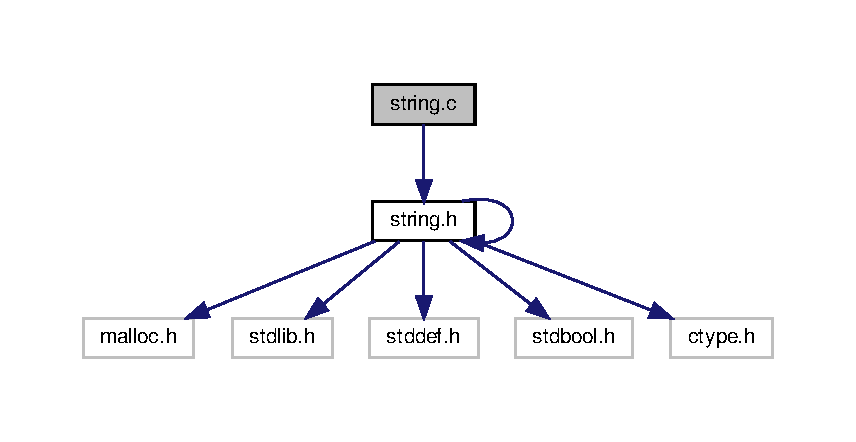
\includegraphics[width=350pt]{string_8c__incl}
\end{center}
\end{figure}
\subsection*{Functions}
\begin{DoxyCompactItemize}
\item 
\hyperlink{string_8h_a3d2981d9da3e25dd89371059777fdd12}{string} $\ast$ \hyperlink{string_8c_aa821400448b382e43edc3d8876702a23}{string\+\_\+new} (size\+\_\+t capacity)
\begin{DoxyCompactList}\small\item\em creates a new string with the given capacity allocates memory with calloc that needs to be freed by string\+\_\+free \end{DoxyCompactList}\item 
void \hyperlink{string_8c_a5254fab9c967057ff11ca5e4499b1185}{string\+\_\+realloc} (\hyperlink{string_8h_a3d2981d9da3e25dd89371059777fdd12}{string} $\ast$str, size\+\_\+t new\+Cap)
\item 
\hyperlink{string_8h_a3d2981d9da3e25dd89371059777fdd12}{string} $\ast$ \hyperlink{string_8c_ab35ab77e02fc70c813d6a3fec85e24b7}{string\+\_\+copy} (\hyperlink{string_8h_a3d2981d9da3e25dd89371059777fdd12}{string} $\ast$str)
\begin{DoxyCompactList}\small\item\em creates a identical copy of a given string allocates memory with calloc that needs to be freed by string\+\_\+free \end{DoxyCompactList}\item 
void \hyperlink{string_8c_ae2382692d1ce97cad773afcee42bf052}{string\+\_\+free} (\hyperlink{string_8h_a3d2981d9da3e25dd89371059777fdd12}{string} $\ast$str)
\begin{DoxyCompactList}\small\item\em frees a string \end{DoxyCompactList}\item 
void \hyperlink{string_8c_a603235a840d0a092758fde1523e1d008}{string\+\_\+concat} (\hyperlink{string_8h_a3d2981d9da3e25dd89371059777fdd12}{string} $\ast$str, char $\ast$src)
\begin{DoxyCompactList}\small\item\em appends src to str \end{DoxyCompactList}\item 
void \hyperlink{string_8c_ac87036e19cb16961895f4cb479d4045b}{string\+\_\+add\+\_\+char} (\hyperlink{string_8h_a3d2981d9da3e25dd89371059777fdd12}{string} $\ast$str, char c)
\begin{DoxyCompactList}\small\item\em adds a char to a string that may be reallocated if capacity isn\textquotesingle{}t big enough \end{DoxyCompactList}\item 
\hyperlink{string_8h_a3d2981d9da3e25dd89371059777fdd12}{string} $\ast$ \hyperlink{string_8c_aad102a2295f103ad210e82c70e7e5abc}{string\+\_\+strip} (\hyperlink{string_8h_a3d2981d9da3e25dd89371059777fdd12}{string} $\ast$str)
\begin{DoxyCompactList}\small\item\em removes all spaces at begin and end of a string \end{DoxyCompactList}\item 
bool \hyperlink{string_8c_ae17ab6b716d38701b59bdce3e336af5b}{string\+\_\+compare} (\hyperlink{string_8h_a3d2981d9da3e25dd89371059777fdd12}{string} $\ast$string1, \hyperlink{string_8h_a3d2981d9da3e25dd89371059777fdd12}{string} $\ast$string2)
\begin{DoxyCompactList}\small\item\em compares two strings compares two string with memcmp \end{DoxyCompactList}\item 
void \hyperlink{string_8c_aec23e8825ca68414bdc4a92e3c1e0f4c}{string\+\_\+print} (\hyperlink{string_8h_a3d2981d9da3e25dd89371059777fdd12}{string} $\ast$str)
\begin{DoxyCompactList}\small\item\em prints a string onto the console \end{DoxyCompactList}\item 
void \hyperlink{string_8c_a106a9cb5d566f892f43d69b1a39e03d0}{string\+\_\+concat\+\_\+str} (\hyperlink{string_8h_a3d2981d9da3e25dd89371059777fdd12}{string} $\ast$dst, \hyperlink{string_8h_a3d2981d9da3e25dd89371059777fdd12}{string} $\ast$src)
\begin{DoxyCompactList}\small\item\em concat string typed string src to dst equivalent to string\+\_\+concat \end{DoxyCompactList}\item 
\hyperlink{string_8h_a3d2981d9da3e25dd89371059777fdd12}{string} $\ast$ \hyperlink{string_8c_ab0ddc9b8b3923b0e4335107a83ba5646}{int\+\_\+to\+\_\+string} (int i)
\begin{DoxyCompactList}\small\item\em int to string function \end{DoxyCompactList}\item 
char $\ast$ \hyperlink{string_8c_aa711f56eb8b3ff42f34a7558a8851623}{int\+\_\+to\+\_\+\+Ascii\+\_\+char} (int i)
\item 
\hyperlink{string_8h_a3d2981d9da3e25dd89371059777fdd12}{string} $\ast$$\ast$ \hyperlink{string_8c_ae2e788f64b141e2298a5cfd2d87fa04c}{string\+\_\+split} (\hyperlink{string_8h_a3d2981d9da3e25dd89371059777fdd12}{string} $\ast$str, char splitter, int $\ast$splits)
\begin{DoxyCompactList}\small\item\em splits a string by c its a basic method with a rather bad runtime of O(2n) if there is a splitter, the list will contain an empty string at the end \end{DoxyCompactList}\item 
\hyperlink{string_8h_a3d2981d9da3e25dd89371059777fdd12}{string} $\ast$ \hyperlink{string_8c_aba2621fcbf1e796c89c0016c7ee62181}{string\+\_\+terminate} (\hyperlink{string_8h_a3d2981d9da3e25dd89371059777fdd12}{string} $\ast$str)
\begin{DoxyCompactList}\small\item\em terminates a string (adds a \textbackslash{}0 to the end). Needed for functions like fopen \end{DoxyCompactList}\item 
long \hyperlink{string_8c_a45399868bf99479d9f2c29261ba9c522}{string\+\_\+to\+\_\+long} (\hyperlink{string_8h_a3d2981d9da3e25dd89371059777fdd12}{string} $\ast$str, int base)
\begin{DoxyCompactList}\small\item\em wrapper for strtol \end{DoxyCompactList}\item 
bool \hyperlink{string_8c_ad50608a8cca672be3290bba079743433}{string\+\_\+compare\+\_\+cstr} (\hyperlink{string_8h_a3d2981d9da3e25dd89371059777fdd12}{string} $\ast$string1, char $\ast$string2)
\begin{DoxyCompactList}\small\item\em little extension to the string\+\_\+compare \end{DoxyCompactList}\item 
\hyperlink{string_8h_a3d2981d9da3e25dd89371059777fdd12}{string} $\ast$ \hyperlink{string_8c_a9391b9b97412980c1b1c4d38378f5543}{string\+\_\+new\+\_\+from\+\_\+cstr} (char $\ast$str)
\begin{DoxyCompactList}\small\item\em creates new string from given char$\ast$ \end{DoxyCompactList}\item 
\hyperlink{string_8h_a3d2981d9da3e25dd89371059777fdd12}{string} $\ast$ \hyperlink{string_8c_a91787f1ed4754b46f73e4cc98e55138c}{string\+\_\+join} (\hyperlink{string_8h_a3d2981d9da3e25dd89371059777fdd12}{string} $\ast$$\ast$splitted, int splits, char separator)
\begin{DoxyCompactList}\small\item\em recombines list from string\+\_\+split function returns null on failure or if splitted is null or if splits is 0. the separator is added between the splits (who would have expected), if non is wanted set separator to 0 \end{DoxyCompactList}\item 
void \hyperlink{string_8c_ac32f628d3a9fe9291a6a52ee79105f73}{string\+\_\+insert} (\hyperlink{string_8h_a3d2981d9da3e25dd89371059777fdd12}{string} $\ast$dst, \hyperlink{string_8h_a3d2981d9da3e25dd89371059777fdd12}{string} $\ast$src, int index)
\begin{DoxyCompactList}\small\item\em inserts src at index \end{DoxyCompactList}\item 
void \hyperlink{string_8c_a84eea55e0341c16a4e5d08d6ad347ab8}{string\+\_\+insert\+\_\+cstr} (\hyperlink{string_8h_a3d2981d9da3e25dd89371059777fdd12}{string} $\ast$dst, char $\ast$src, int index)
\begin{DoxyCompactList}\small\item\em extension of string\+\_\+insert to support char$\ast$ \end{DoxyCompactList}\item 
bool \hyperlink{string_8c_a94d3d0d6464cedb43aeaa204ebd2b7bb}{string\+\_\+startswith} (\hyperlink{string_8h_a3d2981d9da3e25dd89371059777fdd12}{string} $\ast$str, \hyperlink{string_8h_a3d2981d9da3e25dd89371059777fdd12}{string} $\ast$needle)
\begin{DoxyCompactList}\small\item\em checks is str starts with needle uses string\+\_\+compare \end{DoxyCompactList}\item 
bool \hyperlink{string_8c_ab3ed9ef0b1f2464fdfe520e5dc4a380f}{string\+\_\+startswith\+\_\+cstr} (\hyperlink{string_8h_a3d2981d9da3e25dd89371059777fdd12}{string} $\ast$str, char $\ast$needle)
\begin{DoxyCompactList}\small\item\em checks if str starts with needle \end{DoxyCompactList}\item 
bool \hyperlink{string_8c_a37a30efaac2743ae8339f60e54ba6c89}{string\+\_\+endswith} (\hyperlink{string_8h_a3d2981d9da3e25dd89371059777fdd12}{string} $\ast$str, \hyperlink{string_8h_a3d2981d9da3e25dd89371059777fdd12}{string} $\ast$part)
\begin{DoxyCompactList}\small\item\em compares end of string with another string \end{DoxyCompactList}\item 
bool \hyperlink{string_8c_a136d1913d88e81d3aee44c2a9684a41f}{string\+\_\+endswith\+\_\+cstr} (\hyperlink{string_8h_a3d2981d9da3e25dd89371059777fdd12}{string} $\ast$str, char $\ast$part)
\begin{DoxyCompactList}\small\item\em compars end of string with another string (char pointer) \end{DoxyCompactList}\item 
void \hyperlink{string_8c_a54b21c9c9a0df76610c09bf104077243}{move\+\_\+string\+\_\+x\+\_\+left} (\hyperlink{string_8h_a3d2981d9da3e25dd89371059777fdd12}{string} $\ast$str, int x)
\item 
\hyperlink{string_8h_a3d2981d9da3e25dd89371059777fdd12}{string} $\ast$$\ast$ \hyperlink{string_8c_a52c1bfcbbba22c50f093cf5faafe14b3}{string\+\_\+split\+\_\+string} (\hyperlink{string_8h_a3d2981d9da3e25dd89371059777fdd12}{string} $\ast$str, \hyperlink{string_8h_a3d2981d9da3e25dd89371059777fdd12}{string} $\ast$splitter, int $\ast$splits)
\begin{DoxyCompactList}\small\item\em splits a string, but uses a string as splitter argument uses the same \char`\"{}algorithm\char`\"{} as string\+\_\+split but adapted to use string as splitter \end{DoxyCompactList}\item 
\hyperlink{string_8h_a3d2981d9da3e25dd89371059777fdd12}{string} $\ast$$\ast$ \hyperlink{string_8c_a4d2488155e1f18d5d14a9ff3e35df882}{string\+\_\+split\+\_\+cstr} (\hyperlink{string_8h_a3d2981d9da3e25dd89371059777fdd12}{string} $\ast$str, char $\ast$splitter, int $\ast$splits)
\item 
\hyperlink{string_8h_a3d2981d9da3e25dd89371059777fdd12}{string} $\ast$ \hyperlink{string_8c_a7e5d0900b56b765ccd1a668c9a9a4c39}{string\+\_\+new\+\_\+from\+\_\+carray} (char $\ast$str, int len)
\begin{DoxyCompactList}\small\item\em creates new string from given char$\ast$ but limits at length \end{DoxyCompactList}\item 
void \hyperlink{string_8c_a128a94234e54e046f65279d296ddb35b}{string\+\_\+to\+\_\+lower} (\hyperlink{string_8h_a3d2981d9da3e25dd89371059777fdd12}{string} $\ast$str)
\begin{DoxyCompactList}\small\item\em replaces all uppercase chars with lowercase this fuction uses ctypes own tolower function \end{DoxyCompactList}\item 
void \hyperlink{string_8c_a2ac6b2f5bb299fd17fa2804698d2127a}{string\+\_\+free\+\_\+stringlist} (\hyperlink{string_8h_a3d2981d9da3e25dd89371059777fdd12}{string} $\ast$$\ast$list, int num\+Of\+Elements)
\begin{DoxyCompactList}\small\item\em frees a list of \end{DoxyCompactList}\end{DoxyCompactItemize}


\subsection{Function Documentation}
\mbox{\Hypertarget{string_8c_aa711f56eb8b3ff42f34a7558a8851623}\label{string_8c_aa711f56eb8b3ff42f34a7558a8851623}} 
\index{string.\+c@{string.\+c}!int\+\_\+to\+\_\+\+Ascii\+\_\+char@{int\+\_\+to\+\_\+\+Ascii\+\_\+char}}
\index{int\+\_\+to\+\_\+\+Ascii\+\_\+char@{int\+\_\+to\+\_\+\+Ascii\+\_\+char}!string.\+c@{string.\+c}}
\subsubsection{\texorpdfstring{int\+\_\+to\+\_\+\+Ascii\+\_\+char()}{int\_to\_Ascii\_char()}}
{\footnotesize\ttfamily char$\ast$ int\+\_\+to\+\_\+\+Ascii\+\_\+char (\begin{DoxyParamCaption}\item[{int}]{i }\end{DoxyParamCaption})}

\mbox{\Hypertarget{string_8c_ab0ddc9b8b3923b0e4335107a83ba5646}\label{string_8c_ab0ddc9b8b3923b0e4335107a83ba5646}} 
\index{string.\+c@{string.\+c}!int\+\_\+to\+\_\+string@{int\+\_\+to\+\_\+string}}
\index{int\+\_\+to\+\_\+string@{int\+\_\+to\+\_\+string}!string.\+c@{string.\+c}}
\subsubsection{\texorpdfstring{int\+\_\+to\+\_\+string()}{int\_to\_string()}}
{\footnotesize\ttfamily \hyperlink{string_8h_a3d2981d9da3e25dd89371059777fdd12}{string}$\ast$ int\+\_\+to\+\_\+string (\begin{DoxyParamCaption}\item[{int}]{i }\end{DoxyParamCaption})}



int to string function 

\begin{DoxyAuthor}{Author}
Björn Marx
\end{DoxyAuthor}

\begin{DoxyParams}{Parameters}
{\em i} & an integer \\
\hline
\end{DoxyParams}
\begin{DoxyReturn}{Returns}
string containing i 
\end{DoxyReturn}
\mbox{\Hypertarget{string_8c_a54b21c9c9a0df76610c09bf104077243}\label{string_8c_a54b21c9c9a0df76610c09bf104077243}} 
\index{string.\+c@{string.\+c}!move\+\_\+string\+\_\+x\+\_\+left@{move\+\_\+string\+\_\+x\+\_\+left}}
\index{move\+\_\+string\+\_\+x\+\_\+left@{move\+\_\+string\+\_\+x\+\_\+left}!string.\+c@{string.\+c}}
\subsubsection{\texorpdfstring{move\+\_\+string\+\_\+x\+\_\+left()}{move\_string\_x\_left()}}
{\footnotesize\ttfamily void move\+\_\+string\+\_\+x\+\_\+left (\begin{DoxyParamCaption}\item[{\hyperlink{string_8h_a3d2981d9da3e25dd89371059777fdd12}{string} $\ast$}]{str,  }\item[{int}]{x }\end{DoxyParamCaption})}

\mbox{\Hypertarget{string_8c_ac87036e19cb16961895f4cb479d4045b}\label{string_8c_ac87036e19cb16961895f4cb479d4045b}} 
\index{string.\+c@{string.\+c}!string\+\_\+add\+\_\+char@{string\+\_\+add\+\_\+char}}
\index{string\+\_\+add\+\_\+char@{string\+\_\+add\+\_\+char}!string.\+c@{string.\+c}}
\subsubsection{\texorpdfstring{string\+\_\+add\+\_\+char()}{string\_add\_char()}}
{\footnotesize\ttfamily void string\+\_\+add\+\_\+char (\begin{DoxyParamCaption}\item[{\hyperlink{string_8h_a3d2981d9da3e25dd89371059777fdd12}{string} $\ast$}]{str,  }\item[{char}]{c }\end{DoxyParamCaption})}



adds a char to a string that may be reallocated if capacity isn\textquotesingle{}t big enough 

\begin{DoxyAuthor}{Author}
Marcel Weski 
\end{DoxyAuthor}

\begin{DoxyParams}{Parameters}
{\em str} & string to add char to \\
\hline
{\em c} & the char \\
\hline
\end{DoxyParams}
\mbox{\Hypertarget{string_8c_ae17ab6b716d38701b59bdce3e336af5b}\label{string_8c_ae17ab6b716d38701b59bdce3e336af5b}} 
\index{string.\+c@{string.\+c}!string\+\_\+compare@{string\+\_\+compare}}
\index{string\+\_\+compare@{string\+\_\+compare}!string.\+c@{string.\+c}}
\subsubsection{\texorpdfstring{string\+\_\+compare()}{string\_compare()}}
{\footnotesize\ttfamily bool string\+\_\+compare (\begin{DoxyParamCaption}\item[{\hyperlink{string_8h_a3d2981d9da3e25dd89371059777fdd12}{string} $\ast$}]{string1,  }\item[{\hyperlink{string_8h_a3d2981d9da3e25dd89371059777fdd12}{string} $\ast$}]{string2 }\end{DoxyParamCaption})}



compares two strings compares two string with memcmp 

\begin{DoxyAuthor}{Author}
Björn Marx
\end{DoxyAuthor}

\begin{DoxyParams}{Parameters}
{\em string1} & \\
\hline
{\em string2} & \\
\hline
\end{DoxyParams}
\begin{DoxyReturn}{Returns}
true if string1 == string2 
\end{DoxyReturn}
\mbox{\Hypertarget{string_8c_ad50608a8cca672be3290bba079743433}\label{string_8c_ad50608a8cca672be3290bba079743433}} 
\index{string.\+c@{string.\+c}!string\+\_\+compare\+\_\+cstr@{string\+\_\+compare\+\_\+cstr}}
\index{string\+\_\+compare\+\_\+cstr@{string\+\_\+compare\+\_\+cstr}!string.\+c@{string.\+c}}
\subsubsection{\texorpdfstring{string\+\_\+compare\+\_\+cstr()}{string\_compare\_cstr()}}
{\footnotesize\ttfamily bool string\+\_\+compare\+\_\+cstr (\begin{DoxyParamCaption}\item[{\hyperlink{string_8h_a3d2981d9da3e25dd89371059777fdd12}{string} $\ast$}]{string1,  }\item[{char $\ast$}]{string2 }\end{DoxyParamCaption})}



little extension to the string\+\_\+compare 

\begin{DoxyAuthor}{Author}
Björn Marx 
\end{DoxyAuthor}

\begin{DoxyParams}{Parameters}
{\em string1} & a string \\
\hline
{\em string2} & a cstring (char$\ast$) \\
\hline
\end{DoxyParams}
\begin{DoxyReturn}{Returns}
true if equal 
\end{DoxyReturn}
\mbox{\Hypertarget{string_8c_a603235a840d0a092758fde1523e1d008}\label{string_8c_a603235a840d0a092758fde1523e1d008}} 
\index{string.\+c@{string.\+c}!string\+\_\+concat@{string\+\_\+concat}}
\index{string\+\_\+concat@{string\+\_\+concat}!string.\+c@{string.\+c}}
\subsubsection{\texorpdfstring{string\+\_\+concat()}{string\_concat()}}
{\footnotesize\ttfamily void string\+\_\+concat (\begin{DoxyParamCaption}\item[{\hyperlink{string_8h_a3d2981d9da3e25dd89371059777fdd12}{string} $\ast$}]{str,  }\item[{char $\ast$}]{src }\end{DoxyParamCaption})}



appends src to str 

\begin{DoxyAuthor}{Author}
Björn Marx
\end{DoxyAuthor}

\begin{DoxyParams}{Parameters}
{\em str} & string to append to \\
\hline
{\em src} & string to append \\
\hline
\end{DoxyParams}
\mbox{\Hypertarget{string_8c_a106a9cb5d566f892f43d69b1a39e03d0}\label{string_8c_a106a9cb5d566f892f43d69b1a39e03d0}} 
\index{string.\+c@{string.\+c}!string\+\_\+concat\+\_\+str@{string\+\_\+concat\+\_\+str}}
\index{string\+\_\+concat\+\_\+str@{string\+\_\+concat\+\_\+str}!string.\+c@{string.\+c}}
\subsubsection{\texorpdfstring{string\+\_\+concat\+\_\+str()}{string\_concat\_str()}}
{\footnotesize\ttfamily void string\+\_\+concat\+\_\+str (\begin{DoxyParamCaption}\item[{\hyperlink{string_8h_a3d2981d9da3e25dd89371059777fdd12}{string} $\ast$}]{dst,  }\item[{\hyperlink{string_8h_a3d2981d9da3e25dd89371059777fdd12}{string} $\ast$}]{src }\end{DoxyParamCaption})}



concat string typed string src to dst equivalent to string\+\_\+concat 

\begin{DoxyAuthor}{Author}
Björn Marx
\end{DoxyAuthor}

\begin{DoxyParams}{Parameters}
{\em dst} & destination \\
\hline
{\em src} & source \\
\hline
\end{DoxyParams}
\mbox{\Hypertarget{string_8c_ab35ab77e02fc70c813d6a3fec85e24b7}\label{string_8c_ab35ab77e02fc70c813d6a3fec85e24b7}} 
\index{string.\+c@{string.\+c}!string\+\_\+copy@{string\+\_\+copy}}
\index{string\+\_\+copy@{string\+\_\+copy}!string.\+c@{string.\+c}}
\subsubsection{\texorpdfstring{string\+\_\+copy()}{string\_copy()}}
{\footnotesize\ttfamily \hyperlink{string_8h_a3d2981d9da3e25dd89371059777fdd12}{string}$\ast$ string\+\_\+copy (\begin{DoxyParamCaption}\item[{\hyperlink{string_8h_a3d2981d9da3e25dd89371059777fdd12}{string} $\ast$}]{str }\end{DoxyParamCaption})}



creates a identical copy of a given string allocates memory with calloc that needs to be freed by string\+\_\+free 

\begin{DoxyAuthor}{Author}
Marcel Weski 
\end{DoxyAuthor}

\begin{DoxyParams}{Parameters}
{\em str} & string to copy \\
\hline
\end{DoxyParams}
\begin{DoxyReturn}{Returns}
pointer to the new string struct 
\end{DoxyReturn}
\mbox{\Hypertarget{string_8c_a37a30efaac2743ae8339f60e54ba6c89}\label{string_8c_a37a30efaac2743ae8339f60e54ba6c89}} 
\index{string.\+c@{string.\+c}!string\+\_\+endswith@{string\+\_\+endswith}}
\index{string\+\_\+endswith@{string\+\_\+endswith}!string.\+c@{string.\+c}}
\subsubsection{\texorpdfstring{string\+\_\+endswith()}{string\_endswith()}}
{\footnotesize\ttfamily bool string\+\_\+endswith (\begin{DoxyParamCaption}\item[{\hyperlink{string_8h_a3d2981d9da3e25dd89371059777fdd12}{string} $\ast$}]{str,  }\item[{\hyperlink{string_8h_a3d2981d9da3e25dd89371059777fdd12}{string} $\ast$}]{part }\end{DoxyParamCaption})}



compares end of string with another string 

\begin{DoxyAuthor}{Author}
Marcel Weski 
\end{DoxyAuthor}

\begin{DoxyParams}{Parameters}
{\em str} & string to compare end with \\
\hline
{\em part} & end part of str \\
\hline
\end{DoxyParams}
\begin{DoxyReturn}{Returns}
true, if part is equal to last chars of str 
\end{DoxyReturn}
\mbox{\Hypertarget{string_8c_a136d1913d88e81d3aee44c2a9684a41f}\label{string_8c_a136d1913d88e81d3aee44c2a9684a41f}} 
\index{string.\+c@{string.\+c}!string\+\_\+endswith\+\_\+cstr@{string\+\_\+endswith\+\_\+cstr}}
\index{string\+\_\+endswith\+\_\+cstr@{string\+\_\+endswith\+\_\+cstr}!string.\+c@{string.\+c}}
\subsubsection{\texorpdfstring{string\+\_\+endswith\+\_\+cstr()}{string\_endswith\_cstr()}}
{\footnotesize\ttfamily bool string\+\_\+endswith\+\_\+cstr (\begin{DoxyParamCaption}\item[{\hyperlink{string_8h_a3d2981d9da3e25dd89371059777fdd12}{string} $\ast$}]{str,  }\item[{char $\ast$}]{part }\end{DoxyParamCaption})}



compars end of string with another string (char pointer) 

\begin{DoxyAuthor}{Author}
Björn Marx
\end{DoxyAuthor}
\begin{DoxySeeAlso}{See also}
\hyperlink{string_8h_a37a30efaac2743ae8339f60e54ba6c89}{string\+\_\+endswith} 
\end{DoxySeeAlso}
\mbox{\Hypertarget{string_8c_ae2382692d1ce97cad773afcee42bf052}\label{string_8c_ae2382692d1ce97cad773afcee42bf052}} 
\index{string.\+c@{string.\+c}!string\+\_\+free@{string\+\_\+free}}
\index{string\+\_\+free@{string\+\_\+free}!string.\+c@{string.\+c}}
\subsubsection{\texorpdfstring{string\+\_\+free()}{string\_free()}}
{\footnotesize\ttfamily void string\+\_\+free (\begin{DoxyParamCaption}\item[{\hyperlink{string_8h_a3d2981d9da3e25dd89371059777fdd12}{string} $\ast$}]{str }\end{DoxyParamCaption})}



frees a string 

\begin{DoxyAuthor}{Author}
Marcel Weski 
\end{DoxyAuthor}

\begin{DoxyParams}{Parameters}
{\em str} & string to free \\
\hline
\end{DoxyParams}
\mbox{\Hypertarget{string_8c_a2ac6b2f5bb299fd17fa2804698d2127a}\label{string_8c_a2ac6b2f5bb299fd17fa2804698d2127a}} 
\index{string.\+c@{string.\+c}!string\+\_\+free\+\_\+stringlist@{string\+\_\+free\+\_\+stringlist}}
\index{string\+\_\+free\+\_\+stringlist@{string\+\_\+free\+\_\+stringlist}!string.\+c@{string.\+c}}
\subsubsection{\texorpdfstring{string\+\_\+free\+\_\+stringlist()}{string\_free\_stringlist()}}
{\footnotesize\ttfamily void string\+\_\+free\+\_\+stringlist (\begin{DoxyParamCaption}\item[{\hyperlink{string_8h_a3d2981d9da3e25dd89371059777fdd12}{string} $\ast$$\ast$}]{list,  }\item[{int}]{num\+Of\+Elements }\end{DoxyParamCaption})}



frees a list of 


\begin{DoxyParams}{Parameters}
{\em num\+Of\+Elements} & elements\\
\hline
\end{DoxyParams}
\begin{DoxyAuthor}{Author}
Björn Marx
\end{DoxyAuthor}

\begin{DoxyParams}{Parameters}
{\em list} & a stringlist \\
\hline
{\em num\+Of\+Elements} & number of elements in \\
\hline
{\em list} & \\
\hline
\end{DoxyParams}
\mbox{\Hypertarget{string_8c_ac32f628d3a9fe9291a6a52ee79105f73}\label{string_8c_ac32f628d3a9fe9291a6a52ee79105f73}} 
\index{string.\+c@{string.\+c}!string\+\_\+insert@{string\+\_\+insert}}
\index{string\+\_\+insert@{string\+\_\+insert}!string.\+c@{string.\+c}}
\subsubsection{\texorpdfstring{string\+\_\+insert()}{string\_insert()}}
{\footnotesize\ttfamily void string\+\_\+insert (\begin{DoxyParamCaption}\item[{\hyperlink{string_8h_a3d2981d9da3e25dd89371059777fdd12}{string} $\ast$}]{dst,  }\item[{\hyperlink{string_8h_a3d2981d9da3e25dd89371059777fdd12}{string} $\ast$}]{src,  }\item[{int}]{index }\end{DoxyParamCaption})}



inserts src at index 

\begin{DoxyAuthor}{Author}
Björn marx
\end{DoxyAuthor}

\begin{DoxyParams}{Parameters}
{\em dst} & string to insert to \\
\hline
{\em src} & string to insert from \\
\hline
{\em index} & explains itself \\
\hline
\end{DoxyParams}
\mbox{\Hypertarget{string_8c_a84eea55e0341c16a4e5d08d6ad347ab8}\label{string_8c_a84eea55e0341c16a4e5d08d6ad347ab8}} 
\index{string.\+c@{string.\+c}!string\+\_\+insert\+\_\+cstr@{string\+\_\+insert\+\_\+cstr}}
\index{string\+\_\+insert\+\_\+cstr@{string\+\_\+insert\+\_\+cstr}!string.\+c@{string.\+c}}
\subsubsection{\texorpdfstring{string\+\_\+insert\+\_\+cstr()}{string\_insert\_cstr()}}
{\footnotesize\ttfamily void string\+\_\+insert\+\_\+cstr (\begin{DoxyParamCaption}\item[{\hyperlink{string_8h_a3d2981d9da3e25dd89371059777fdd12}{string} $\ast$}]{dst,  }\item[{char $\ast$}]{src,  }\item[{int}]{index }\end{DoxyParamCaption})}



extension of string\+\_\+insert to support char$\ast$ 

\begin{DoxyAuthor}{Author}
Björn Marx 
\end{DoxyAuthor}
\begin{DoxySeeAlso}{See also}
\hyperlink{string_8h_ac32f628d3a9fe9291a6a52ee79105f73}{string\+\_\+insert} 
\end{DoxySeeAlso}
\mbox{\Hypertarget{string_8c_a91787f1ed4754b46f73e4cc98e55138c}\label{string_8c_a91787f1ed4754b46f73e4cc98e55138c}} 
\index{string.\+c@{string.\+c}!string\+\_\+join@{string\+\_\+join}}
\index{string\+\_\+join@{string\+\_\+join}!string.\+c@{string.\+c}}
\subsubsection{\texorpdfstring{string\+\_\+join()}{string\_join()}}
{\footnotesize\ttfamily \hyperlink{string_8h_a3d2981d9da3e25dd89371059777fdd12}{string}$\ast$ string\+\_\+join (\begin{DoxyParamCaption}\item[{\hyperlink{string_8h_a3d2981d9da3e25dd89371059777fdd12}{string} $\ast$$\ast$}]{splitted,  }\item[{int}]{splits,  }\item[{char}]{separator }\end{DoxyParamCaption})}



recombines list from string\+\_\+split function returns null on failure or if splitted is null or if splits is 0. the separator is added between the splits (who would have expected), if non is wanted set separator to 0 

\begin{DoxyAuthor}{Author}
Björn Marx
\end{DoxyAuthor}

\begin{DoxyParams}{Parameters}
{\em splitted} & list of splitted strings \\
\hline
{\em splits} & number of strings in splitted \\
\hline
{\em separator} & char to put between individual strings \\
\hline
\end{DoxyParams}
\begin{DoxyReturn}{Returns}
string containing all substrings of splitted 
\end{DoxyReturn}
\mbox{\Hypertarget{string_8c_aa821400448b382e43edc3d8876702a23}\label{string_8c_aa821400448b382e43edc3d8876702a23}} 
\index{string.\+c@{string.\+c}!string\+\_\+new@{string\+\_\+new}}
\index{string\+\_\+new@{string\+\_\+new}!string.\+c@{string.\+c}}
\subsubsection{\texorpdfstring{string\+\_\+new()}{string\_new()}}
{\footnotesize\ttfamily \hyperlink{string_8h_a3d2981d9da3e25dd89371059777fdd12}{string}$\ast$ string\+\_\+new (\begin{DoxyParamCaption}\item[{size\+\_\+t}]{capacity }\end{DoxyParamCaption})}



creates a new string with the given capacity allocates memory with calloc that needs to be freed by string\+\_\+free 

\begin{DoxyAuthor}{Author}
Marcel Weski 
\end{DoxyAuthor}

\begin{DoxyParams}{Parameters}
{\em capacity} & max. amount of chars that can be saved before reallocating \\
\hline
\end{DoxyParams}
\begin{DoxyReturn}{Returns}
pointer to string struct 
\end{DoxyReturn}
\mbox{\Hypertarget{string_8c_a7e5d0900b56b765ccd1a668c9a9a4c39}\label{string_8c_a7e5d0900b56b765ccd1a668c9a9a4c39}} 
\index{string.\+c@{string.\+c}!string\+\_\+new\+\_\+from\+\_\+carray@{string\+\_\+new\+\_\+from\+\_\+carray}}
\index{string\+\_\+new\+\_\+from\+\_\+carray@{string\+\_\+new\+\_\+from\+\_\+carray}!string.\+c@{string.\+c}}
\subsubsection{\texorpdfstring{string\+\_\+new\+\_\+from\+\_\+carray()}{string\_new\_from\_carray()}}
{\footnotesize\ttfamily \hyperlink{string_8h_a3d2981d9da3e25dd89371059777fdd12}{string}$\ast$ string\+\_\+new\+\_\+from\+\_\+carray (\begin{DoxyParamCaption}\item[{char $\ast$}]{str,  }\item[{int}]{len }\end{DoxyParamCaption})}



creates new string from given char$\ast$ but limits at length 

\begin{DoxyAuthor}{Author}
Björn Marx
\end{DoxyAuthor}

\begin{DoxyParams}{Parameters}
{\em str} & a char$\ast$ \\
\hline
{\em len} & length of char$\ast$ \\
\hline
\end{DoxyParams}
\begin{DoxyReturn}{Returns}
new string 
\end{DoxyReturn}
\mbox{\Hypertarget{string_8c_a9391b9b97412980c1b1c4d38378f5543}\label{string_8c_a9391b9b97412980c1b1c4d38378f5543}} 
\index{string.\+c@{string.\+c}!string\+\_\+new\+\_\+from\+\_\+cstr@{string\+\_\+new\+\_\+from\+\_\+cstr}}
\index{string\+\_\+new\+\_\+from\+\_\+cstr@{string\+\_\+new\+\_\+from\+\_\+cstr}!string.\+c@{string.\+c}}
\subsubsection{\texorpdfstring{string\+\_\+new\+\_\+from\+\_\+cstr()}{string\_new\_from\_cstr()}}
{\footnotesize\ttfamily \hyperlink{string_8h_a3d2981d9da3e25dd89371059777fdd12}{string}$\ast$ string\+\_\+new\+\_\+from\+\_\+cstr (\begin{DoxyParamCaption}\item[{char $\ast$}]{str }\end{DoxyParamCaption})}



creates new string from given char$\ast$ 

\begin{DoxyAuthor}{Author}
Björn Marx
\end{DoxyAuthor}

\begin{DoxyParams}{Parameters}
{\em str} & a string \\
\hline
\end{DoxyParams}
\begin{DoxyReturn}{Returns}
new string with content of str, N\+U\+LL if 
\end{DoxyReturn}

\begin{DoxyParams}{Parameters}
{\em str} & is N\+U\+LL \\
\hline
\end{DoxyParams}
\mbox{\Hypertarget{string_8c_aec23e8825ca68414bdc4a92e3c1e0f4c}\label{string_8c_aec23e8825ca68414bdc4a92e3c1e0f4c}} 
\index{string.\+c@{string.\+c}!string\+\_\+print@{string\+\_\+print}}
\index{string\+\_\+print@{string\+\_\+print}!string.\+c@{string.\+c}}
\subsubsection{\texorpdfstring{string\+\_\+print()}{string\_print()}}
{\footnotesize\ttfamily void string\+\_\+print (\begin{DoxyParamCaption}\item[{\hyperlink{string_8h_a3d2981d9da3e25dd89371059777fdd12}{string} $\ast$}]{str }\end{DoxyParamCaption})}



prints a string onto the console 

\begin{DoxyAuthor}{Author}
Marcel Weski 
\end{DoxyAuthor}

\begin{DoxyParams}{Parameters}
{\em str} & String \\
\hline
\end{DoxyParams}
\mbox{\Hypertarget{string_8c_a5254fab9c967057ff11ca5e4499b1185}\label{string_8c_a5254fab9c967057ff11ca5e4499b1185}} 
\index{string.\+c@{string.\+c}!string\+\_\+realloc@{string\+\_\+realloc}}
\index{string\+\_\+realloc@{string\+\_\+realloc}!string.\+c@{string.\+c}}
\subsubsection{\texorpdfstring{string\+\_\+realloc()}{string\_realloc()}}
{\footnotesize\ttfamily void string\+\_\+realloc (\begin{DoxyParamCaption}\item[{\hyperlink{string_8h_a3d2981d9da3e25dd89371059777fdd12}{string} $\ast$}]{str,  }\item[{size\+\_\+t}]{new\+Cap }\end{DoxyParamCaption})}

\mbox{\Hypertarget{string_8c_ae2e788f64b141e2298a5cfd2d87fa04c}\label{string_8c_ae2e788f64b141e2298a5cfd2d87fa04c}} 
\index{string.\+c@{string.\+c}!string\+\_\+split@{string\+\_\+split}}
\index{string\+\_\+split@{string\+\_\+split}!string.\+c@{string.\+c}}
\subsubsection{\texorpdfstring{string\+\_\+split()}{string\_split()}}
{\footnotesize\ttfamily \hyperlink{string_8h_a3d2981d9da3e25dd89371059777fdd12}{string}$\ast$$\ast$ string\+\_\+split (\begin{DoxyParamCaption}\item[{\hyperlink{string_8h_a3d2981d9da3e25dd89371059777fdd12}{string} $\ast$}]{str,  }\item[{char}]{splitter,  }\item[{int $\ast$}]{splits }\end{DoxyParamCaption})}



splits a string by c its a basic method with a rather bad runtime of O(2n) if there is a splitter, the list will contain an empty string at the end 

\begin{DoxyAuthor}{Author}
Björn Marx
\end{DoxyAuthor}

\begin{DoxyParams}{Parameters}
{\em splits} & pointer to integer to store stringlists length in \\
\hline
{\em str} & an string \\
\hline
{\em splitter} & charakter defining when to split \\
\hline
\end{DoxyParams}
\begin{DoxyReturn}{Returns}
list of strings 
\end{DoxyReturn}
\mbox{\Hypertarget{string_8c_a4d2488155e1f18d5d14a9ff3e35df882}\label{string_8c_a4d2488155e1f18d5d14a9ff3e35df882}} 
\index{string.\+c@{string.\+c}!string\+\_\+split\+\_\+cstr@{string\+\_\+split\+\_\+cstr}}
\index{string\+\_\+split\+\_\+cstr@{string\+\_\+split\+\_\+cstr}!string.\+c@{string.\+c}}
\subsubsection{\texorpdfstring{string\+\_\+split\+\_\+cstr()}{string\_split\_cstr()}}
{\footnotesize\ttfamily \hyperlink{string_8h_a3d2981d9da3e25dd89371059777fdd12}{string}$\ast$$\ast$ string\+\_\+split\+\_\+cstr (\begin{DoxyParamCaption}\item[{\hyperlink{string_8h_a3d2981d9da3e25dd89371059777fdd12}{string} $\ast$}]{str,  }\item[{char $\ast$}]{splitter,  }\item[{int $\ast$}]{splits }\end{DoxyParamCaption})}

\begin{DoxySeeAlso}{See also}
\hyperlink{string_8h_a52c1bfcbbba22c50f093cf5faafe14b3}{string\+\_\+split\+\_\+string}
\end{DoxySeeAlso}
\begin{DoxyAuthor}{Author}
Björn Marx 
\end{DoxyAuthor}
\mbox{\Hypertarget{string_8c_a52c1bfcbbba22c50f093cf5faafe14b3}\label{string_8c_a52c1bfcbbba22c50f093cf5faafe14b3}} 
\index{string.\+c@{string.\+c}!string\+\_\+split\+\_\+string@{string\+\_\+split\+\_\+string}}
\index{string\+\_\+split\+\_\+string@{string\+\_\+split\+\_\+string}!string.\+c@{string.\+c}}
\subsubsection{\texorpdfstring{string\+\_\+split\+\_\+string()}{string\_split\_string()}}
{\footnotesize\ttfamily \hyperlink{string_8h_a3d2981d9da3e25dd89371059777fdd12}{string}$\ast$$\ast$ string\+\_\+split\+\_\+string (\begin{DoxyParamCaption}\item[{\hyperlink{string_8h_a3d2981d9da3e25dd89371059777fdd12}{string} $\ast$}]{str,  }\item[{\hyperlink{string_8h_a3d2981d9da3e25dd89371059777fdd12}{string} $\ast$}]{splitter,  }\item[{int $\ast$}]{splits }\end{DoxyParamCaption})}



splits a string, but uses a string as splitter argument uses the same \char`\"{}algorithm\char`\"{} as string\+\_\+split but adapted to use string as splitter 

\begin{DoxyAuthor}{Author}
Björn Marx
\end{DoxyAuthor}

\begin{DoxyParams}{Parameters}
{\em str} & string to split \\
\hline
{\em splitter} & string that splits \\
\hline
{\em splits} & number of splits \\
\hline
\end{DoxyParams}
\begin{DoxyReturn}{Returns}
array of splitted string 
\end{DoxyReturn}
\mbox{\Hypertarget{string_8c_a94d3d0d6464cedb43aeaa204ebd2b7bb}\label{string_8c_a94d3d0d6464cedb43aeaa204ebd2b7bb}} 
\index{string.\+c@{string.\+c}!string\+\_\+startswith@{string\+\_\+startswith}}
\index{string\+\_\+startswith@{string\+\_\+startswith}!string.\+c@{string.\+c}}
\subsubsection{\texorpdfstring{string\+\_\+startswith()}{string\_startswith()}}
{\footnotesize\ttfamily bool string\+\_\+startswith (\begin{DoxyParamCaption}\item[{\hyperlink{string_8h_a3d2981d9da3e25dd89371059777fdd12}{string} $\ast$}]{str,  }\item[{\hyperlink{string_8h_a3d2981d9da3e25dd89371059777fdd12}{string} $\ast$}]{needle }\end{DoxyParamCaption})}



checks is str starts with needle uses string\+\_\+compare 

\begin{DoxySeeAlso}{See also}
\hyperlink{string_8h_ae17ab6b716d38701b59bdce3e336af5b}{string\+\_\+compare} for detailed info
\end{DoxySeeAlso}
\begin{DoxyAuthor}{Author}
Björn Marx
\end{DoxyAuthor}

\begin{DoxyParams}{Parameters}
{\em str} & string to check if it starts with needle \\
\hline
{\em needle} & a string \\
\hline
\end{DoxyParams}
\begin{DoxyReturn}{Returns}
true if string starts with needle 
\end{DoxyReturn}
\mbox{\Hypertarget{string_8c_ab3ed9ef0b1f2464fdfe520e5dc4a380f}\label{string_8c_ab3ed9ef0b1f2464fdfe520e5dc4a380f}} 
\index{string.\+c@{string.\+c}!string\+\_\+startswith\+\_\+cstr@{string\+\_\+startswith\+\_\+cstr}}
\index{string\+\_\+startswith\+\_\+cstr@{string\+\_\+startswith\+\_\+cstr}!string.\+c@{string.\+c}}
\subsubsection{\texorpdfstring{string\+\_\+startswith\+\_\+cstr()}{string\_startswith\_cstr()}}
{\footnotesize\ttfamily bool string\+\_\+startswith\+\_\+cstr (\begin{DoxyParamCaption}\item[{\hyperlink{string_8h_a3d2981d9da3e25dd89371059777fdd12}{string} $\ast$}]{str,  }\item[{char $\ast$}]{needle }\end{DoxyParamCaption})}



checks if str starts with needle 

\begin{DoxyAuthor}{Author}
Björn Marx
\end{DoxyAuthor}
\begin{DoxySeeAlso}{See also}
\hyperlink{string_8h_a94d3d0d6464cedb43aeaa204ebd2b7bb}{string\+\_\+startswith} to see how it works 
\end{DoxySeeAlso}
\mbox{\Hypertarget{string_8c_aad102a2295f103ad210e82c70e7e5abc}\label{string_8c_aad102a2295f103ad210e82c70e7e5abc}} 
\index{string.\+c@{string.\+c}!string\+\_\+strip@{string\+\_\+strip}}
\index{string\+\_\+strip@{string\+\_\+strip}!string.\+c@{string.\+c}}
\subsubsection{\texorpdfstring{string\+\_\+strip()}{string\_strip()}}
{\footnotesize\ttfamily \hyperlink{string_8h_a3d2981d9da3e25dd89371059777fdd12}{string}$\ast$ string\+\_\+strip (\begin{DoxyParamCaption}\item[{\hyperlink{string_8h_a3d2981d9da3e25dd89371059777fdd12}{string} $\ast$}]{str }\end{DoxyParamCaption})}



removes all spaces at begin and end of a string 

\begin{DoxyAuthor}{Author}
Marcel Weski 
\end{DoxyAuthor}

\begin{DoxyParams}{Parameters}
{\em str} & string to be stripped \\
\hline
\end{DoxyParams}
\mbox{\Hypertarget{string_8c_aba2621fcbf1e796c89c0016c7ee62181}\label{string_8c_aba2621fcbf1e796c89c0016c7ee62181}} 
\index{string.\+c@{string.\+c}!string\+\_\+terminate@{string\+\_\+terminate}}
\index{string\+\_\+terminate@{string\+\_\+terminate}!string.\+c@{string.\+c}}
\subsubsection{\texorpdfstring{string\+\_\+terminate()}{string\_terminate()}}
{\footnotesize\ttfamily \hyperlink{string_8h_a3d2981d9da3e25dd89371059777fdd12}{string}$\ast$ string\+\_\+terminate (\begin{DoxyParamCaption}\item[{\hyperlink{string_8h_a3d2981d9da3e25dd89371059777fdd12}{string} $\ast$}]{str }\end{DoxyParamCaption})}



terminates a string (adds a \textbackslash{}0 to the end). Needed for functions like fopen 

\begin{DoxyAuthor}{Author}
Marcel Weski 
\end{DoxyAuthor}

\begin{DoxyParams}{Parameters}
{\em str} & string to terminate \\
\hline
\end{DoxyParams}
\begin{DoxyReturn}{Returns}
same string as argument (never changes, just to make code more compact) 
\end{DoxyReturn}
\mbox{\Hypertarget{string_8c_a45399868bf99479d9f2c29261ba9c522}\label{string_8c_a45399868bf99479d9f2c29261ba9c522}} 
\index{string.\+c@{string.\+c}!string\+\_\+to\+\_\+long@{string\+\_\+to\+\_\+long}}
\index{string\+\_\+to\+\_\+long@{string\+\_\+to\+\_\+long}!string.\+c@{string.\+c}}
\subsubsection{\texorpdfstring{string\+\_\+to\+\_\+long()}{string\_to\_long()}}
{\footnotesize\ttfamily long string\+\_\+to\+\_\+long (\begin{DoxyParamCaption}\item[{\hyperlink{string_8h_a3d2981d9da3e25dd89371059777fdd12}{string} $\ast$}]{str,  }\item[{int}]{base }\end{DoxyParamCaption})}



wrapper for strtol 

\begin{DoxyAuthor}{Author}
Björn Marx
\end{DoxyAuthor}

\begin{DoxyParams}{Parameters}
{\em str} & \\
\hline
\end{DoxyParams}
\begin{DoxyReturn}{Returns}

\end{DoxyReturn}
\mbox{\Hypertarget{string_8c_a128a94234e54e046f65279d296ddb35b}\label{string_8c_a128a94234e54e046f65279d296ddb35b}} 
\index{string.\+c@{string.\+c}!string\+\_\+to\+\_\+lower@{string\+\_\+to\+\_\+lower}}
\index{string\+\_\+to\+\_\+lower@{string\+\_\+to\+\_\+lower}!string.\+c@{string.\+c}}
\subsubsection{\texorpdfstring{string\+\_\+to\+\_\+lower()}{string\_to\_lower()}}
{\footnotesize\ttfamily void string\+\_\+to\+\_\+lower (\begin{DoxyParamCaption}\item[{\hyperlink{string_8h_a3d2981d9da3e25dd89371059777fdd12}{string} $\ast$}]{str }\end{DoxyParamCaption})}



replaces all uppercase chars with lowercase this fuction uses ctypes own tolower function 

\begin{DoxyAuthor}{Author}
Björn Marx
\end{DoxyAuthor}

\begin{DoxyParams}{Parameters}
{\em str} & a string \\
\hline
\end{DoxyParams}

\hypertarget{string_8h}{}\section{string.\+h File Reference}
\label{string_8h}\index{string.\+h@{string.\+h}}
{\ttfamily \#include $<$malloc.\+h$>$}\newline
{\ttfamily \#include $<$stdlib.\+h$>$}\newline
{\ttfamily \#include $<$stddef.\+h$>$}\newline
{\ttfamily \#include $<$string.\+h$>$}\newline
{\ttfamily \#include $<$stdbool.\+h$>$}\newline
{\ttfamily \#include $<$ctype.\+h$>$}\newline
Include dependency graph for string.\+h\+:
\nopagebreak
\begin{figure}[H]
\begin{center}
\leavevmode
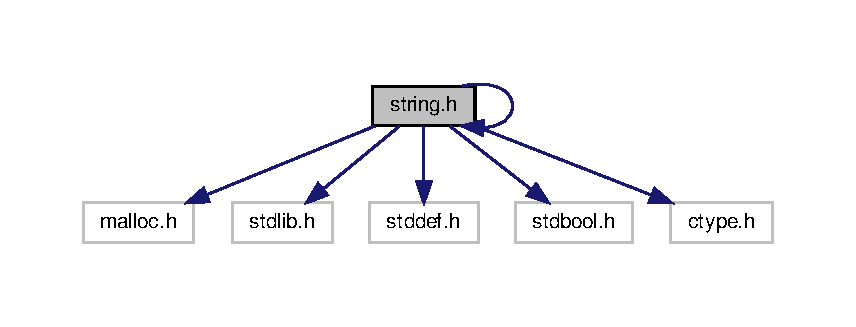
\includegraphics[width=350pt]{string_8h__incl}
\end{center}
\end{figure}
This graph shows which files directly or indirectly include this file\+:
\nopagebreak
\begin{figure}[H]
\begin{center}
\leavevmode
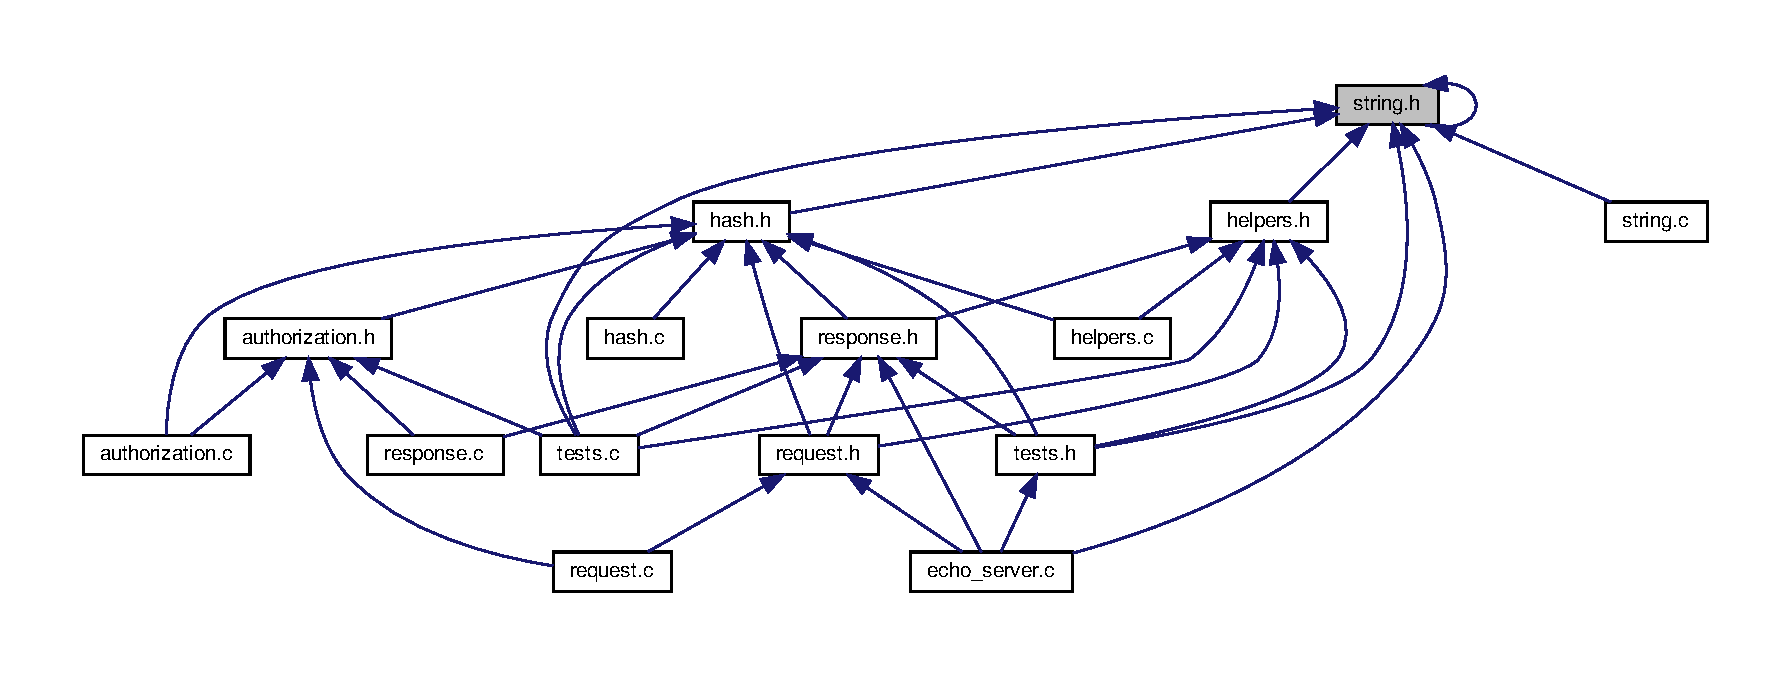
\includegraphics[width=350pt]{string_8h__dep__incl}
\end{center}
\end{figure}
\subsection*{Data Structures}
\begin{DoxyCompactItemize}
\item 
struct \hyperlink{structstring__struct}{string\+\_\+struct}
\end{DoxyCompactItemize}
\subsection*{Typedefs}
\begin{DoxyCompactItemize}
\item 
typedef struct \hyperlink{structstring__struct}{string\+\_\+struct} \hyperlink{string_8h_a3d2981d9da3e25dd89371059777fdd12}{string}
\end{DoxyCompactItemize}
\subsection*{Functions}
\begin{DoxyCompactItemize}
\item 
\hyperlink{string_8h_a3d2981d9da3e25dd89371059777fdd12}{string} $\ast$ \hyperlink{string_8h_aa821400448b382e43edc3d8876702a23}{string\+\_\+new} (size\+\_\+t capacity)
\begin{DoxyCompactList}\small\item\em creates a new string with the given capacity allocates memory with calloc that needs to be freed by string\+\_\+free \end{DoxyCompactList}\item 
\hyperlink{string_8h_a3d2981d9da3e25dd89371059777fdd12}{string} $\ast$ \hyperlink{string_8h_a9391b9b97412980c1b1c4d38378f5543}{string\+\_\+new\+\_\+from\+\_\+cstr} (char $\ast$str)
\begin{DoxyCompactList}\small\item\em creates new string from given char$\ast$ \end{DoxyCompactList}\item 
\hyperlink{string_8h_a3d2981d9da3e25dd89371059777fdd12}{string} $\ast$ \hyperlink{string_8h_a7e5d0900b56b765ccd1a668c9a9a4c39}{string\+\_\+new\+\_\+from\+\_\+carray} (char $\ast$str, int len)
\begin{DoxyCompactList}\small\item\em creates new string from given char$\ast$ but limits at length \end{DoxyCompactList}\item 
\hyperlink{string_8h_a3d2981d9da3e25dd89371059777fdd12}{string} $\ast$ \hyperlink{string_8h_ab35ab77e02fc70c813d6a3fec85e24b7}{string\+\_\+copy} (\hyperlink{string_8h_a3d2981d9da3e25dd89371059777fdd12}{string} $\ast$str)
\begin{DoxyCompactList}\small\item\em creates a identical copy of a given string allocates memory with calloc that needs to be freed by string\+\_\+free \end{DoxyCompactList}\item 
void \hyperlink{string_8h_ae2382692d1ce97cad773afcee42bf052}{string\+\_\+free} (\hyperlink{string_8h_a3d2981d9da3e25dd89371059777fdd12}{string} $\ast$str)
\begin{DoxyCompactList}\small\item\em frees a string \end{DoxyCompactList}\item 
void \hyperlink{string_8h_a603235a840d0a092758fde1523e1d008}{string\+\_\+concat} (\hyperlink{string_8h_a3d2981d9da3e25dd89371059777fdd12}{string} $\ast$str, char $\ast$src)
\begin{DoxyCompactList}\small\item\em appends src to str \end{DoxyCompactList}\item 
void \hyperlink{string_8h_a106a9cb5d566f892f43d69b1a39e03d0}{string\+\_\+concat\+\_\+str} (\hyperlink{string_8h_a3d2981d9da3e25dd89371059777fdd12}{string} $\ast$dst, \hyperlink{string_8h_a3d2981d9da3e25dd89371059777fdd12}{string} $\ast$src)
\begin{DoxyCompactList}\small\item\em concat string typed string src to dst equivalent to string\+\_\+concat \end{DoxyCompactList}\item 
void \hyperlink{string_8h_ac87036e19cb16961895f4cb479d4045b}{string\+\_\+add\+\_\+char} (\hyperlink{string_8h_a3d2981d9da3e25dd89371059777fdd12}{string} $\ast$str, char c)
\begin{DoxyCompactList}\small\item\em adds a char to a string that may be reallocated if capacity isn\textquotesingle{}t big enough \end{DoxyCompactList}\item 
\hyperlink{string_8h_a3d2981d9da3e25dd89371059777fdd12}{string} $\ast$ \hyperlink{string_8h_aad102a2295f103ad210e82c70e7e5abc}{string\+\_\+strip} (\hyperlink{string_8h_a3d2981d9da3e25dd89371059777fdd12}{string} $\ast$str)
\begin{DoxyCompactList}\small\item\em removes all spaces at begin and end of a string \end{DoxyCompactList}\item 
bool \hyperlink{string_8h_ae17ab6b716d38701b59bdce3e336af5b}{string\+\_\+compare} (\hyperlink{string_8h_a3d2981d9da3e25dd89371059777fdd12}{string} $\ast$string1, \hyperlink{string_8h_a3d2981d9da3e25dd89371059777fdd12}{string} $\ast$string2)
\begin{DoxyCompactList}\small\item\em compares two strings compares two string with memcmp \end{DoxyCompactList}\item 
void \hyperlink{string_8h_aec23e8825ca68414bdc4a92e3c1e0f4c}{string\+\_\+print} (\hyperlink{string_8h_a3d2981d9da3e25dd89371059777fdd12}{string} $\ast$str)
\begin{DoxyCompactList}\small\item\em prints a string onto the console \end{DoxyCompactList}\item 
\hyperlink{string_8h_a3d2981d9da3e25dd89371059777fdd12}{string} $\ast$ \hyperlink{string_8h_ab0ddc9b8b3923b0e4335107a83ba5646}{int\+\_\+to\+\_\+string} (int i)
\begin{DoxyCompactList}\small\item\em int to string function \end{DoxyCompactList}\item 
long \hyperlink{string_8h_a45399868bf99479d9f2c29261ba9c522}{string\+\_\+to\+\_\+long} (\hyperlink{string_8h_a3d2981d9da3e25dd89371059777fdd12}{string} $\ast$str, int base)
\begin{DoxyCompactList}\small\item\em wrapper for strtol \end{DoxyCompactList}\item 
\hyperlink{string_8h_a3d2981d9da3e25dd89371059777fdd12}{string} $\ast$$\ast$ \hyperlink{string_8h_ae2e788f64b141e2298a5cfd2d87fa04c}{string\+\_\+split} (\hyperlink{string_8h_a3d2981d9da3e25dd89371059777fdd12}{string} $\ast$str, char splitter, int $\ast$splits)
\begin{DoxyCompactList}\small\item\em splits a string by c its a basic method with a rather bad runtime of O(2n) if there is a splitter, the list will contain an empty string at the end \end{DoxyCompactList}\item 
\hyperlink{string_8h_a3d2981d9da3e25dd89371059777fdd12}{string} $\ast$$\ast$ \hyperlink{string_8h_a52c1bfcbbba22c50f093cf5faafe14b3}{string\+\_\+split\+\_\+string} (\hyperlink{string_8h_a3d2981d9da3e25dd89371059777fdd12}{string} $\ast$str, \hyperlink{string_8h_a3d2981d9da3e25dd89371059777fdd12}{string} $\ast$splitter, int $\ast$splits)
\begin{DoxyCompactList}\small\item\em splits a string, but uses a string as splitter argument uses the same \char`\"{}algorithm\char`\"{} as string\+\_\+split but adapted to use string as splitter \end{DoxyCompactList}\item 
\hyperlink{string_8h_a3d2981d9da3e25dd89371059777fdd12}{string} $\ast$$\ast$ \hyperlink{string_8h_a4d2488155e1f18d5d14a9ff3e35df882}{string\+\_\+split\+\_\+cstr} (\hyperlink{string_8h_a3d2981d9da3e25dd89371059777fdd12}{string} $\ast$str, char $\ast$splitter, int $\ast$splits)
\item 
\hyperlink{string_8h_a3d2981d9da3e25dd89371059777fdd12}{string} $\ast$ \hyperlink{string_8h_a91787f1ed4754b46f73e4cc98e55138c}{string\+\_\+join} (\hyperlink{string_8h_a3d2981d9da3e25dd89371059777fdd12}{string} $\ast$$\ast$splitted, int splits, char separator)
\begin{DoxyCompactList}\small\item\em recombines list from string\+\_\+split function returns null on failure or if splitted is null or if splits is 0. the separator is added between the splits (who would have expected), if non is wanted set separator to 0 \end{DoxyCompactList}\item 
\hyperlink{string_8h_a3d2981d9da3e25dd89371059777fdd12}{string} $\ast$ \hyperlink{string_8h_aba2621fcbf1e796c89c0016c7ee62181}{string\+\_\+terminate} (\hyperlink{string_8h_a3d2981d9da3e25dd89371059777fdd12}{string} $\ast$str)
\begin{DoxyCompactList}\small\item\em terminates a string (adds a \textbackslash{}0 to the end). Needed for functions like fopen \end{DoxyCompactList}\item 
bool \hyperlink{string_8h_ad50608a8cca672be3290bba079743433}{string\+\_\+compare\+\_\+cstr} (\hyperlink{string_8h_a3d2981d9da3e25dd89371059777fdd12}{string} $\ast$string1, char $\ast$string2)
\begin{DoxyCompactList}\small\item\em little extension to the string\+\_\+compare \end{DoxyCompactList}\item 
void \hyperlink{string_8h_ac32f628d3a9fe9291a6a52ee79105f73}{string\+\_\+insert} (\hyperlink{string_8h_a3d2981d9da3e25dd89371059777fdd12}{string} $\ast$dst, \hyperlink{string_8h_a3d2981d9da3e25dd89371059777fdd12}{string} $\ast$src, int index)
\begin{DoxyCompactList}\small\item\em inserts src at index \end{DoxyCompactList}\item 
void \hyperlink{string_8h_a84eea55e0341c16a4e5d08d6ad347ab8}{string\+\_\+insert\+\_\+cstr} (\hyperlink{string_8h_a3d2981d9da3e25dd89371059777fdd12}{string} $\ast$dst, char $\ast$src, int index)
\begin{DoxyCompactList}\small\item\em extension of string\+\_\+insert to support char$\ast$ \end{DoxyCompactList}\item 
bool \hyperlink{string_8h_a94d3d0d6464cedb43aeaa204ebd2b7bb}{string\+\_\+startswith} (\hyperlink{string_8h_a3d2981d9da3e25dd89371059777fdd12}{string} $\ast$str, \hyperlink{string_8h_a3d2981d9da3e25dd89371059777fdd12}{string} $\ast$needle)
\begin{DoxyCompactList}\small\item\em checks is str starts with needle uses string\+\_\+compare \end{DoxyCompactList}\item 
bool \hyperlink{string_8h_ab3ed9ef0b1f2464fdfe520e5dc4a380f}{string\+\_\+startswith\+\_\+cstr} (\hyperlink{string_8h_a3d2981d9da3e25dd89371059777fdd12}{string} $\ast$str, char $\ast$needle)
\begin{DoxyCompactList}\small\item\em checks if str starts with needle \end{DoxyCompactList}\item 
bool \hyperlink{string_8h_a37a30efaac2743ae8339f60e54ba6c89}{string\+\_\+endswith} (\hyperlink{string_8h_a3d2981d9da3e25dd89371059777fdd12}{string} $\ast$str, \hyperlink{string_8h_a3d2981d9da3e25dd89371059777fdd12}{string} $\ast$part)
\begin{DoxyCompactList}\small\item\em compares end of string with another string \end{DoxyCompactList}\item 
bool \hyperlink{string_8h_a136d1913d88e81d3aee44c2a9684a41f}{string\+\_\+endswith\+\_\+cstr} (\hyperlink{string_8h_a3d2981d9da3e25dd89371059777fdd12}{string} $\ast$str, char $\ast$part)
\begin{DoxyCompactList}\small\item\em compars end of string with another string (char pointer) \end{DoxyCompactList}\item 
void \hyperlink{string_8h_a128a94234e54e046f65279d296ddb35b}{string\+\_\+to\+\_\+lower} (\hyperlink{string_8h_a3d2981d9da3e25dd89371059777fdd12}{string} $\ast$str)
\begin{DoxyCompactList}\small\item\em replaces all uppercase chars with lowercase this fuction uses ctypes own tolower function \end{DoxyCompactList}\item 
void \hyperlink{string_8h_a2ac6b2f5bb299fd17fa2804698d2127a}{string\+\_\+free\+\_\+stringlist} (\hyperlink{string_8h_a3d2981d9da3e25dd89371059777fdd12}{string} $\ast$$\ast$list, int num\+Of\+Elements)
\begin{DoxyCompactList}\small\item\em frees a list of \end{DoxyCompactList}\end{DoxyCompactItemize}


\subsection{Detailed Description}
\begin{DoxyAuthor}{Author}
Björn Marx 

Marcel Weski 
\end{DoxyAuthor}


\subsection{Typedef Documentation}
\mbox{\Hypertarget{string_8h_a3d2981d9da3e25dd89371059777fdd12}\label{string_8h_a3d2981d9da3e25dd89371059777fdd12}} 
\index{string.\+h@{string.\+h}!string@{string}}
\index{string@{string}!string.\+h@{string.\+h}}
\subsubsection{\texorpdfstring{string}{string}}
{\footnotesize\ttfamily typedef struct \hyperlink{structstring__struct}{string\+\_\+struct}  \hyperlink{string_8h_a3d2981d9da3e25dd89371059777fdd12}{string}}



\subsection{Function Documentation}
\mbox{\Hypertarget{string_8h_ab0ddc9b8b3923b0e4335107a83ba5646}\label{string_8h_ab0ddc9b8b3923b0e4335107a83ba5646}} 
\index{string.\+h@{string.\+h}!int\+\_\+to\+\_\+string@{int\+\_\+to\+\_\+string}}
\index{int\+\_\+to\+\_\+string@{int\+\_\+to\+\_\+string}!string.\+h@{string.\+h}}
\subsubsection{\texorpdfstring{int\+\_\+to\+\_\+string()}{int\_to\_string()}}
{\footnotesize\ttfamily \hyperlink{string_8h_a3d2981d9da3e25dd89371059777fdd12}{string}$\ast$ int\+\_\+to\+\_\+string (\begin{DoxyParamCaption}\item[{int}]{i }\end{DoxyParamCaption})}



int to string function 

\begin{DoxyAuthor}{Author}
Björn Marx
\end{DoxyAuthor}

\begin{DoxyParams}{Parameters}
{\em i} & an integer \\
\hline
\end{DoxyParams}
\begin{DoxyReturn}{Returns}
string containing i 
\end{DoxyReturn}
\mbox{\Hypertarget{string_8h_ac87036e19cb16961895f4cb479d4045b}\label{string_8h_ac87036e19cb16961895f4cb479d4045b}} 
\index{string.\+h@{string.\+h}!string\+\_\+add\+\_\+char@{string\+\_\+add\+\_\+char}}
\index{string\+\_\+add\+\_\+char@{string\+\_\+add\+\_\+char}!string.\+h@{string.\+h}}
\subsubsection{\texorpdfstring{string\+\_\+add\+\_\+char()}{string\_add\_char()}}
{\footnotesize\ttfamily void string\+\_\+add\+\_\+char (\begin{DoxyParamCaption}\item[{\hyperlink{string_8h_a3d2981d9da3e25dd89371059777fdd12}{string} $\ast$}]{str,  }\item[{char}]{c }\end{DoxyParamCaption})}



adds a char to a string that may be reallocated if capacity isn\textquotesingle{}t big enough 

\begin{DoxyAuthor}{Author}
Marcel Weski 
\end{DoxyAuthor}

\begin{DoxyParams}{Parameters}
{\em str} & string to add char to \\
\hline
{\em c} & the char \\
\hline
\end{DoxyParams}
\mbox{\Hypertarget{string_8h_ae17ab6b716d38701b59bdce3e336af5b}\label{string_8h_ae17ab6b716d38701b59bdce3e336af5b}} 
\index{string.\+h@{string.\+h}!string\+\_\+compare@{string\+\_\+compare}}
\index{string\+\_\+compare@{string\+\_\+compare}!string.\+h@{string.\+h}}
\subsubsection{\texorpdfstring{string\+\_\+compare()}{string\_compare()}}
{\footnotesize\ttfamily bool string\+\_\+compare (\begin{DoxyParamCaption}\item[{\hyperlink{string_8h_a3d2981d9da3e25dd89371059777fdd12}{string} $\ast$}]{string1,  }\item[{\hyperlink{string_8h_a3d2981d9da3e25dd89371059777fdd12}{string} $\ast$}]{string2 }\end{DoxyParamCaption})}



compares two strings compares two string with memcmp 

\begin{DoxyAuthor}{Author}
Björn Marx
\end{DoxyAuthor}

\begin{DoxyParams}{Parameters}
{\em string1} & \\
\hline
{\em string2} & \\
\hline
\end{DoxyParams}
\begin{DoxyReturn}{Returns}
true if string1 == string2 
\end{DoxyReturn}
\mbox{\Hypertarget{string_8h_ad50608a8cca672be3290bba079743433}\label{string_8h_ad50608a8cca672be3290bba079743433}} 
\index{string.\+h@{string.\+h}!string\+\_\+compare\+\_\+cstr@{string\+\_\+compare\+\_\+cstr}}
\index{string\+\_\+compare\+\_\+cstr@{string\+\_\+compare\+\_\+cstr}!string.\+h@{string.\+h}}
\subsubsection{\texorpdfstring{string\+\_\+compare\+\_\+cstr()}{string\_compare\_cstr()}}
{\footnotesize\ttfamily bool string\+\_\+compare\+\_\+cstr (\begin{DoxyParamCaption}\item[{\hyperlink{string_8h_a3d2981d9da3e25dd89371059777fdd12}{string} $\ast$}]{string1,  }\item[{char $\ast$}]{string2 }\end{DoxyParamCaption})}



little extension to the string\+\_\+compare 

\begin{DoxyAuthor}{Author}
Björn Marx 
\end{DoxyAuthor}

\begin{DoxyParams}{Parameters}
{\em string1} & a string \\
\hline
{\em string2} & a cstring (char$\ast$) \\
\hline
\end{DoxyParams}
\begin{DoxyReturn}{Returns}
true if equal 
\end{DoxyReturn}
\mbox{\Hypertarget{string_8h_a603235a840d0a092758fde1523e1d008}\label{string_8h_a603235a840d0a092758fde1523e1d008}} 
\index{string.\+h@{string.\+h}!string\+\_\+concat@{string\+\_\+concat}}
\index{string\+\_\+concat@{string\+\_\+concat}!string.\+h@{string.\+h}}
\subsubsection{\texorpdfstring{string\+\_\+concat()}{string\_concat()}}
{\footnotesize\ttfamily void string\+\_\+concat (\begin{DoxyParamCaption}\item[{\hyperlink{string_8h_a3d2981d9da3e25dd89371059777fdd12}{string} $\ast$}]{str,  }\item[{char $\ast$}]{src }\end{DoxyParamCaption})}



appends src to str 

\begin{DoxyAuthor}{Author}
Björn Marx
\end{DoxyAuthor}

\begin{DoxyParams}{Parameters}
{\em str} & string to append to \\
\hline
{\em src} & string to append \\
\hline
\end{DoxyParams}
\mbox{\Hypertarget{string_8h_a106a9cb5d566f892f43d69b1a39e03d0}\label{string_8h_a106a9cb5d566f892f43d69b1a39e03d0}} 
\index{string.\+h@{string.\+h}!string\+\_\+concat\+\_\+str@{string\+\_\+concat\+\_\+str}}
\index{string\+\_\+concat\+\_\+str@{string\+\_\+concat\+\_\+str}!string.\+h@{string.\+h}}
\subsubsection{\texorpdfstring{string\+\_\+concat\+\_\+str()}{string\_concat\_str()}}
{\footnotesize\ttfamily void string\+\_\+concat\+\_\+str (\begin{DoxyParamCaption}\item[{\hyperlink{string_8h_a3d2981d9da3e25dd89371059777fdd12}{string} $\ast$}]{dst,  }\item[{\hyperlink{string_8h_a3d2981d9da3e25dd89371059777fdd12}{string} $\ast$}]{src }\end{DoxyParamCaption})}



concat string typed string src to dst equivalent to string\+\_\+concat 

\begin{DoxyAuthor}{Author}
Björn Marx
\end{DoxyAuthor}

\begin{DoxyParams}{Parameters}
{\em dst} & destination \\
\hline
{\em src} & source \\
\hline
\end{DoxyParams}
\mbox{\Hypertarget{string_8h_ab35ab77e02fc70c813d6a3fec85e24b7}\label{string_8h_ab35ab77e02fc70c813d6a3fec85e24b7}} 
\index{string.\+h@{string.\+h}!string\+\_\+copy@{string\+\_\+copy}}
\index{string\+\_\+copy@{string\+\_\+copy}!string.\+h@{string.\+h}}
\subsubsection{\texorpdfstring{string\+\_\+copy()}{string\_copy()}}
{\footnotesize\ttfamily \hyperlink{string_8h_a3d2981d9da3e25dd89371059777fdd12}{string}$\ast$ string\+\_\+copy (\begin{DoxyParamCaption}\item[{\hyperlink{string_8h_a3d2981d9da3e25dd89371059777fdd12}{string} $\ast$}]{str }\end{DoxyParamCaption})}



creates a identical copy of a given string allocates memory with calloc that needs to be freed by string\+\_\+free 

\begin{DoxyAuthor}{Author}
Marcel Weski 
\end{DoxyAuthor}

\begin{DoxyParams}{Parameters}
{\em str} & string to copy \\
\hline
\end{DoxyParams}
\begin{DoxyReturn}{Returns}
pointer to the new string struct 
\end{DoxyReturn}
\mbox{\Hypertarget{string_8h_a37a30efaac2743ae8339f60e54ba6c89}\label{string_8h_a37a30efaac2743ae8339f60e54ba6c89}} 
\index{string.\+h@{string.\+h}!string\+\_\+endswith@{string\+\_\+endswith}}
\index{string\+\_\+endswith@{string\+\_\+endswith}!string.\+h@{string.\+h}}
\subsubsection{\texorpdfstring{string\+\_\+endswith()}{string\_endswith()}}
{\footnotesize\ttfamily bool string\+\_\+endswith (\begin{DoxyParamCaption}\item[{\hyperlink{string_8h_a3d2981d9da3e25dd89371059777fdd12}{string} $\ast$}]{str,  }\item[{\hyperlink{string_8h_a3d2981d9da3e25dd89371059777fdd12}{string} $\ast$}]{part }\end{DoxyParamCaption})}



compares end of string with another string 

\begin{DoxyAuthor}{Author}
Marcel Weski 
\end{DoxyAuthor}

\begin{DoxyParams}{Parameters}
{\em str} & string to compare end with \\
\hline
{\em part} & end part of str \\
\hline
\end{DoxyParams}
\begin{DoxyReturn}{Returns}
true, if part is equal to last chars of str 
\end{DoxyReturn}
\mbox{\Hypertarget{string_8h_a136d1913d88e81d3aee44c2a9684a41f}\label{string_8h_a136d1913d88e81d3aee44c2a9684a41f}} 
\index{string.\+h@{string.\+h}!string\+\_\+endswith\+\_\+cstr@{string\+\_\+endswith\+\_\+cstr}}
\index{string\+\_\+endswith\+\_\+cstr@{string\+\_\+endswith\+\_\+cstr}!string.\+h@{string.\+h}}
\subsubsection{\texorpdfstring{string\+\_\+endswith\+\_\+cstr()}{string\_endswith\_cstr()}}
{\footnotesize\ttfamily bool string\+\_\+endswith\+\_\+cstr (\begin{DoxyParamCaption}\item[{\hyperlink{string_8h_a3d2981d9da3e25dd89371059777fdd12}{string} $\ast$}]{str,  }\item[{char $\ast$}]{part }\end{DoxyParamCaption})}



compars end of string with another string (char pointer) 

\begin{DoxyAuthor}{Author}
Björn Marx
\end{DoxyAuthor}
\begin{DoxySeeAlso}{See also}
\hyperlink{string_8h_a37a30efaac2743ae8339f60e54ba6c89}{string\+\_\+endswith} 
\end{DoxySeeAlso}
\mbox{\Hypertarget{string_8h_ae2382692d1ce97cad773afcee42bf052}\label{string_8h_ae2382692d1ce97cad773afcee42bf052}} 
\index{string.\+h@{string.\+h}!string\+\_\+free@{string\+\_\+free}}
\index{string\+\_\+free@{string\+\_\+free}!string.\+h@{string.\+h}}
\subsubsection{\texorpdfstring{string\+\_\+free()}{string\_free()}}
{\footnotesize\ttfamily void string\+\_\+free (\begin{DoxyParamCaption}\item[{\hyperlink{string_8h_a3d2981d9da3e25dd89371059777fdd12}{string} $\ast$}]{str }\end{DoxyParamCaption})}



frees a string 

\begin{DoxyAuthor}{Author}
Marcel Weski 
\end{DoxyAuthor}

\begin{DoxyParams}{Parameters}
{\em str} & string to free \\
\hline
\end{DoxyParams}
\mbox{\Hypertarget{string_8h_a2ac6b2f5bb299fd17fa2804698d2127a}\label{string_8h_a2ac6b2f5bb299fd17fa2804698d2127a}} 
\index{string.\+h@{string.\+h}!string\+\_\+free\+\_\+stringlist@{string\+\_\+free\+\_\+stringlist}}
\index{string\+\_\+free\+\_\+stringlist@{string\+\_\+free\+\_\+stringlist}!string.\+h@{string.\+h}}
\subsubsection{\texorpdfstring{string\+\_\+free\+\_\+stringlist()}{string\_free\_stringlist()}}
{\footnotesize\ttfamily void string\+\_\+free\+\_\+stringlist (\begin{DoxyParamCaption}\item[{\hyperlink{string_8h_a3d2981d9da3e25dd89371059777fdd12}{string} $\ast$$\ast$}]{list,  }\item[{int}]{num\+Of\+Elements }\end{DoxyParamCaption})}



frees a list of 


\begin{DoxyParams}{Parameters}
{\em num\+Of\+Elements} & elements\\
\hline
\end{DoxyParams}
\begin{DoxyAuthor}{Author}
Björn Marx
\end{DoxyAuthor}

\begin{DoxyParams}{Parameters}
{\em list} & a stringlist \\
\hline
{\em num\+Of\+Elements} & number of elements in \\
\hline
{\em list} & \\
\hline
\end{DoxyParams}
\mbox{\Hypertarget{string_8h_ac32f628d3a9fe9291a6a52ee79105f73}\label{string_8h_ac32f628d3a9fe9291a6a52ee79105f73}} 
\index{string.\+h@{string.\+h}!string\+\_\+insert@{string\+\_\+insert}}
\index{string\+\_\+insert@{string\+\_\+insert}!string.\+h@{string.\+h}}
\subsubsection{\texorpdfstring{string\+\_\+insert()}{string\_insert()}}
{\footnotesize\ttfamily void string\+\_\+insert (\begin{DoxyParamCaption}\item[{\hyperlink{string_8h_a3d2981d9da3e25dd89371059777fdd12}{string} $\ast$}]{dst,  }\item[{\hyperlink{string_8h_a3d2981d9da3e25dd89371059777fdd12}{string} $\ast$}]{src,  }\item[{int}]{index }\end{DoxyParamCaption})}



inserts src at index 

\begin{DoxyAuthor}{Author}
Björn marx
\end{DoxyAuthor}

\begin{DoxyParams}{Parameters}
{\em dst} & string to insert to \\
\hline
{\em src} & string to insert from \\
\hline
{\em index} & explains itself \\
\hline
\end{DoxyParams}
\mbox{\Hypertarget{string_8h_a84eea55e0341c16a4e5d08d6ad347ab8}\label{string_8h_a84eea55e0341c16a4e5d08d6ad347ab8}} 
\index{string.\+h@{string.\+h}!string\+\_\+insert\+\_\+cstr@{string\+\_\+insert\+\_\+cstr}}
\index{string\+\_\+insert\+\_\+cstr@{string\+\_\+insert\+\_\+cstr}!string.\+h@{string.\+h}}
\subsubsection{\texorpdfstring{string\+\_\+insert\+\_\+cstr()}{string\_insert\_cstr()}}
{\footnotesize\ttfamily void string\+\_\+insert\+\_\+cstr (\begin{DoxyParamCaption}\item[{\hyperlink{string_8h_a3d2981d9da3e25dd89371059777fdd12}{string} $\ast$}]{dst,  }\item[{char $\ast$}]{src,  }\item[{int}]{index }\end{DoxyParamCaption})}



extension of string\+\_\+insert to support char$\ast$ 

\begin{DoxyAuthor}{Author}
Björn Marx 
\end{DoxyAuthor}
\begin{DoxySeeAlso}{See also}
\hyperlink{string_8h_ac32f628d3a9fe9291a6a52ee79105f73}{string\+\_\+insert} 
\end{DoxySeeAlso}
\mbox{\Hypertarget{string_8h_a91787f1ed4754b46f73e4cc98e55138c}\label{string_8h_a91787f1ed4754b46f73e4cc98e55138c}} 
\index{string.\+h@{string.\+h}!string\+\_\+join@{string\+\_\+join}}
\index{string\+\_\+join@{string\+\_\+join}!string.\+h@{string.\+h}}
\subsubsection{\texorpdfstring{string\+\_\+join()}{string\_join()}}
{\footnotesize\ttfamily \hyperlink{string_8h_a3d2981d9da3e25dd89371059777fdd12}{string}$\ast$ string\+\_\+join (\begin{DoxyParamCaption}\item[{\hyperlink{string_8h_a3d2981d9da3e25dd89371059777fdd12}{string} $\ast$$\ast$}]{splitted,  }\item[{int}]{splits,  }\item[{char}]{separator }\end{DoxyParamCaption})}



recombines list from string\+\_\+split function returns null on failure or if splitted is null or if splits is 0. the separator is added between the splits (who would have expected), if non is wanted set separator to 0 

\begin{DoxyAuthor}{Author}
Björn Marx
\end{DoxyAuthor}

\begin{DoxyParams}{Parameters}
{\em splitted} & list of splitted strings \\
\hline
{\em splits} & number of strings in splitted \\
\hline
{\em separator} & char to put between individual strings \\
\hline
\end{DoxyParams}
\begin{DoxyReturn}{Returns}
string containing all substrings of splitted 
\end{DoxyReturn}
\mbox{\Hypertarget{string_8h_aa821400448b382e43edc3d8876702a23}\label{string_8h_aa821400448b382e43edc3d8876702a23}} 
\index{string.\+h@{string.\+h}!string\+\_\+new@{string\+\_\+new}}
\index{string\+\_\+new@{string\+\_\+new}!string.\+h@{string.\+h}}
\subsubsection{\texorpdfstring{string\+\_\+new()}{string\_new()}}
{\footnotesize\ttfamily \hyperlink{string_8h_a3d2981d9da3e25dd89371059777fdd12}{string}$\ast$ string\+\_\+new (\begin{DoxyParamCaption}\item[{size\+\_\+t}]{capacity }\end{DoxyParamCaption})}



creates a new string with the given capacity allocates memory with calloc that needs to be freed by string\+\_\+free 

\begin{DoxyAuthor}{Author}
Marcel Weski 
\end{DoxyAuthor}

\begin{DoxyParams}{Parameters}
{\em capacity} & max. amount of chars that can be saved before reallocating \\
\hline
\end{DoxyParams}
\begin{DoxyReturn}{Returns}
pointer to string struct 
\end{DoxyReturn}
\mbox{\Hypertarget{string_8h_a7e5d0900b56b765ccd1a668c9a9a4c39}\label{string_8h_a7e5d0900b56b765ccd1a668c9a9a4c39}} 
\index{string.\+h@{string.\+h}!string\+\_\+new\+\_\+from\+\_\+carray@{string\+\_\+new\+\_\+from\+\_\+carray}}
\index{string\+\_\+new\+\_\+from\+\_\+carray@{string\+\_\+new\+\_\+from\+\_\+carray}!string.\+h@{string.\+h}}
\subsubsection{\texorpdfstring{string\+\_\+new\+\_\+from\+\_\+carray()}{string\_new\_from\_carray()}}
{\footnotesize\ttfamily \hyperlink{string_8h_a3d2981d9da3e25dd89371059777fdd12}{string}$\ast$ string\+\_\+new\+\_\+from\+\_\+carray (\begin{DoxyParamCaption}\item[{char $\ast$}]{str,  }\item[{int}]{len }\end{DoxyParamCaption})}



creates new string from given char$\ast$ but limits at length 

\begin{DoxyAuthor}{Author}
Björn Marx
\end{DoxyAuthor}

\begin{DoxyParams}{Parameters}
{\em str} & a char$\ast$ \\
\hline
{\em len} & length of char$\ast$ \\
\hline
\end{DoxyParams}
\begin{DoxyReturn}{Returns}
new string 
\end{DoxyReturn}
\mbox{\Hypertarget{string_8h_a9391b9b97412980c1b1c4d38378f5543}\label{string_8h_a9391b9b97412980c1b1c4d38378f5543}} 
\index{string.\+h@{string.\+h}!string\+\_\+new\+\_\+from\+\_\+cstr@{string\+\_\+new\+\_\+from\+\_\+cstr}}
\index{string\+\_\+new\+\_\+from\+\_\+cstr@{string\+\_\+new\+\_\+from\+\_\+cstr}!string.\+h@{string.\+h}}
\subsubsection{\texorpdfstring{string\+\_\+new\+\_\+from\+\_\+cstr()}{string\_new\_from\_cstr()}}
{\footnotesize\ttfamily \hyperlink{string_8h_a3d2981d9da3e25dd89371059777fdd12}{string}$\ast$ string\+\_\+new\+\_\+from\+\_\+cstr (\begin{DoxyParamCaption}\item[{char $\ast$}]{str }\end{DoxyParamCaption})}



creates new string from given char$\ast$ 

\begin{DoxyAuthor}{Author}
Björn Marx
\end{DoxyAuthor}

\begin{DoxyParams}{Parameters}
{\em str} & a string \\
\hline
\end{DoxyParams}
\begin{DoxyReturn}{Returns}
new string with content of str, N\+U\+LL if 
\end{DoxyReturn}

\begin{DoxyParams}{Parameters}
{\em str} & is N\+U\+LL \\
\hline
\end{DoxyParams}
\mbox{\Hypertarget{string_8h_aec23e8825ca68414bdc4a92e3c1e0f4c}\label{string_8h_aec23e8825ca68414bdc4a92e3c1e0f4c}} 
\index{string.\+h@{string.\+h}!string\+\_\+print@{string\+\_\+print}}
\index{string\+\_\+print@{string\+\_\+print}!string.\+h@{string.\+h}}
\subsubsection{\texorpdfstring{string\+\_\+print()}{string\_print()}}
{\footnotesize\ttfamily void string\+\_\+print (\begin{DoxyParamCaption}\item[{\hyperlink{string_8h_a3d2981d9da3e25dd89371059777fdd12}{string} $\ast$}]{str }\end{DoxyParamCaption})}



prints a string onto the console 

\begin{DoxyAuthor}{Author}
Marcel Weski 
\end{DoxyAuthor}

\begin{DoxyParams}{Parameters}
{\em str} & String \\
\hline
\end{DoxyParams}
\mbox{\Hypertarget{string_8h_ae2e788f64b141e2298a5cfd2d87fa04c}\label{string_8h_ae2e788f64b141e2298a5cfd2d87fa04c}} 
\index{string.\+h@{string.\+h}!string\+\_\+split@{string\+\_\+split}}
\index{string\+\_\+split@{string\+\_\+split}!string.\+h@{string.\+h}}
\subsubsection{\texorpdfstring{string\+\_\+split()}{string\_split()}}
{\footnotesize\ttfamily \hyperlink{string_8h_a3d2981d9da3e25dd89371059777fdd12}{string}$\ast$$\ast$ string\+\_\+split (\begin{DoxyParamCaption}\item[{\hyperlink{string_8h_a3d2981d9da3e25dd89371059777fdd12}{string} $\ast$}]{str,  }\item[{char}]{splitter,  }\item[{int $\ast$}]{splits }\end{DoxyParamCaption})}



splits a string by c its a basic method with a rather bad runtime of O(2n) if there is a splitter, the list will contain an empty string at the end 

\begin{DoxyAuthor}{Author}
Björn Marx
\end{DoxyAuthor}

\begin{DoxyParams}{Parameters}
{\em splits} & pointer to integer to store stringlists length in \\
\hline
{\em str} & an string \\
\hline
{\em splitter} & charakter defining when to split \\
\hline
\end{DoxyParams}
\begin{DoxyReturn}{Returns}
list of strings 
\end{DoxyReturn}
\mbox{\Hypertarget{string_8h_a4d2488155e1f18d5d14a9ff3e35df882}\label{string_8h_a4d2488155e1f18d5d14a9ff3e35df882}} 
\index{string.\+h@{string.\+h}!string\+\_\+split\+\_\+cstr@{string\+\_\+split\+\_\+cstr}}
\index{string\+\_\+split\+\_\+cstr@{string\+\_\+split\+\_\+cstr}!string.\+h@{string.\+h}}
\subsubsection{\texorpdfstring{string\+\_\+split\+\_\+cstr()}{string\_split\_cstr()}}
{\footnotesize\ttfamily \hyperlink{string_8h_a3d2981d9da3e25dd89371059777fdd12}{string}$\ast$$\ast$ string\+\_\+split\+\_\+cstr (\begin{DoxyParamCaption}\item[{\hyperlink{string_8h_a3d2981d9da3e25dd89371059777fdd12}{string} $\ast$}]{str,  }\item[{char $\ast$}]{splitter,  }\item[{int $\ast$}]{splits }\end{DoxyParamCaption})}

\begin{DoxySeeAlso}{See also}
\hyperlink{string_8h_a52c1bfcbbba22c50f093cf5faafe14b3}{string\+\_\+split\+\_\+string}
\end{DoxySeeAlso}
\begin{DoxyAuthor}{Author}
Björn Marx 
\end{DoxyAuthor}
\mbox{\Hypertarget{string_8h_a52c1bfcbbba22c50f093cf5faafe14b3}\label{string_8h_a52c1bfcbbba22c50f093cf5faafe14b3}} 
\index{string.\+h@{string.\+h}!string\+\_\+split\+\_\+string@{string\+\_\+split\+\_\+string}}
\index{string\+\_\+split\+\_\+string@{string\+\_\+split\+\_\+string}!string.\+h@{string.\+h}}
\subsubsection{\texorpdfstring{string\+\_\+split\+\_\+string()}{string\_split\_string()}}
{\footnotesize\ttfamily \hyperlink{string_8h_a3d2981d9da3e25dd89371059777fdd12}{string}$\ast$$\ast$ string\+\_\+split\+\_\+string (\begin{DoxyParamCaption}\item[{\hyperlink{string_8h_a3d2981d9da3e25dd89371059777fdd12}{string} $\ast$}]{str,  }\item[{\hyperlink{string_8h_a3d2981d9da3e25dd89371059777fdd12}{string} $\ast$}]{splitter,  }\item[{int $\ast$}]{splits }\end{DoxyParamCaption})}



splits a string, but uses a string as splitter argument uses the same \char`\"{}algorithm\char`\"{} as string\+\_\+split but adapted to use string as splitter 

\begin{DoxyAuthor}{Author}
Björn Marx
\end{DoxyAuthor}

\begin{DoxyParams}{Parameters}
{\em str} & string to split \\
\hline
{\em splitter} & string that splits \\
\hline
{\em splits} & number of splits \\
\hline
\end{DoxyParams}
\begin{DoxyReturn}{Returns}
array of splitted string 
\end{DoxyReturn}
\mbox{\Hypertarget{string_8h_a94d3d0d6464cedb43aeaa204ebd2b7bb}\label{string_8h_a94d3d0d6464cedb43aeaa204ebd2b7bb}} 
\index{string.\+h@{string.\+h}!string\+\_\+startswith@{string\+\_\+startswith}}
\index{string\+\_\+startswith@{string\+\_\+startswith}!string.\+h@{string.\+h}}
\subsubsection{\texorpdfstring{string\+\_\+startswith()}{string\_startswith()}}
{\footnotesize\ttfamily bool string\+\_\+startswith (\begin{DoxyParamCaption}\item[{\hyperlink{string_8h_a3d2981d9da3e25dd89371059777fdd12}{string} $\ast$}]{str,  }\item[{\hyperlink{string_8h_a3d2981d9da3e25dd89371059777fdd12}{string} $\ast$}]{needle }\end{DoxyParamCaption})}



checks is str starts with needle uses string\+\_\+compare 

\begin{DoxySeeAlso}{See also}
\hyperlink{string_8h_ae17ab6b716d38701b59bdce3e336af5b}{string\+\_\+compare} for detailed info
\end{DoxySeeAlso}
\begin{DoxyAuthor}{Author}
Björn Marx
\end{DoxyAuthor}

\begin{DoxyParams}{Parameters}
{\em str} & string to check if it starts with needle \\
\hline
{\em needle} & a string \\
\hline
\end{DoxyParams}
\begin{DoxyReturn}{Returns}
true if string starts with needle 
\end{DoxyReturn}
\mbox{\Hypertarget{string_8h_ab3ed9ef0b1f2464fdfe520e5dc4a380f}\label{string_8h_ab3ed9ef0b1f2464fdfe520e5dc4a380f}} 
\index{string.\+h@{string.\+h}!string\+\_\+startswith\+\_\+cstr@{string\+\_\+startswith\+\_\+cstr}}
\index{string\+\_\+startswith\+\_\+cstr@{string\+\_\+startswith\+\_\+cstr}!string.\+h@{string.\+h}}
\subsubsection{\texorpdfstring{string\+\_\+startswith\+\_\+cstr()}{string\_startswith\_cstr()}}
{\footnotesize\ttfamily bool string\+\_\+startswith\+\_\+cstr (\begin{DoxyParamCaption}\item[{\hyperlink{string_8h_a3d2981d9da3e25dd89371059777fdd12}{string} $\ast$}]{str,  }\item[{char $\ast$}]{needle }\end{DoxyParamCaption})}



checks if str starts with needle 

\begin{DoxyAuthor}{Author}
Björn Marx
\end{DoxyAuthor}
\begin{DoxySeeAlso}{See also}
\hyperlink{string_8h_a94d3d0d6464cedb43aeaa204ebd2b7bb}{string\+\_\+startswith} to see how it works 
\end{DoxySeeAlso}
\mbox{\Hypertarget{string_8h_aad102a2295f103ad210e82c70e7e5abc}\label{string_8h_aad102a2295f103ad210e82c70e7e5abc}} 
\index{string.\+h@{string.\+h}!string\+\_\+strip@{string\+\_\+strip}}
\index{string\+\_\+strip@{string\+\_\+strip}!string.\+h@{string.\+h}}
\subsubsection{\texorpdfstring{string\+\_\+strip()}{string\_strip()}}
{\footnotesize\ttfamily \hyperlink{string_8h_a3d2981d9da3e25dd89371059777fdd12}{string}$\ast$ string\+\_\+strip (\begin{DoxyParamCaption}\item[{\hyperlink{string_8h_a3d2981d9da3e25dd89371059777fdd12}{string} $\ast$}]{str }\end{DoxyParamCaption})}



removes all spaces at begin and end of a string 

\begin{DoxyAuthor}{Author}
Marcel Weski 
\end{DoxyAuthor}

\begin{DoxyParams}{Parameters}
{\em str} & string to be stripped \\
\hline
\end{DoxyParams}
\mbox{\Hypertarget{string_8h_aba2621fcbf1e796c89c0016c7ee62181}\label{string_8h_aba2621fcbf1e796c89c0016c7ee62181}} 
\index{string.\+h@{string.\+h}!string\+\_\+terminate@{string\+\_\+terminate}}
\index{string\+\_\+terminate@{string\+\_\+terminate}!string.\+h@{string.\+h}}
\subsubsection{\texorpdfstring{string\+\_\+terminate()}{string\_terminate()}}
{\footnotesize\ttfamily \hyperlink{string_8h_a3d2981d9da3e25dd89371059777fdd12}{string}$\ast$ string\+\_\+terminate (\begin{DoxyParamCaption}\item[{\hyperlink{string_8h_a3d2981d9da3e25dd89371059777fdd12}{string} $\ast$}]{str }\end{DoxyParamCaption})}



terminates a string (adds a \textbackslash{}0 to the end). Needed for functions like fopen 

\begin{DoxyAuthor}{Author}
Marcel Weski 
\end{DoxyAuthor}

\begin{DoxyParams}{Parameters}
{\em str} & string to terminate \\
\hline
\end{DoxyParams}
\begin{DoxyReturn}{Returns}
same string as argument (never changes, just to make code more compact) 
\end{DoxyReturn}
\mbox{\Hypertarget{string_8h_a45399868bf99479d9f2c29261ba9c522}\label{string_8h_a45399868bf99479d9f2c29261ba9c522}} 
\index{string.\+h@{string.\+h}!string\+\_\+to\+\_\+long@{string\+\_\+to\+\_\+long}}
\index{string\+\_\+to\+\_\+long@{string\+\_\+to\+\_\+long}!string.\+h@{string.\+h}}
\subsubsection{\texorpdfstring{string\+\_\+to\+\_\+long()}{string\_to\_long()}}
{\footnotesize\ttfamily long string\+\_\+to\+\_\+long (\begin{DoxyParamCaption}\item[{\hyperlink{string_8h_a3d2981d9da3e25dd89371059777fdd12}{string} $\ast$}]{str,  }\item[{int}]{base }\end{DoxyParamCaption})}



wrapper for strtol 

\begin{DoxyAuthor}{Author}
Björn Marx
\end{DoxyAuthor}

\begin{DoxyParams}{Parameters}
{\em str} & \\
\hline
\end{DoxyParams}
\begin{DoxyReturn}{Returns}

\end{DoxyReturn}
\mbox{\Hypertarget{string_8h_a128a94234e54e046f65279d296ddb35b}\label{string_8h_a128a94234e54e046f65279d296ddb35b}} 
\index{string.\+h@{string.\+h}!string\+\_\+to\+\_\+lower@{string\+\_\+to\+\_\+lower}}
\index{string\+\_\+to\+\_\+lower@{string\+\_\+to\+\_\+lower}!string.\+h@{string.\+h}}
\subsubsection{\texorpdfstring{string\+\_\+to\+\_\+lower()}{string\_to\_lower()}}
{\footnotesize\ttfamily void string\+\_\+to\+\_\+lower (\begin{DoxyParamCaption}\item[{\hyperlink{string_8h_a3d2981d9da3e25dd89371059777fdd12}{string} $\ast$}]{str }\end{DoxyParamCaption})}



replaces all uppercase chars with lowercase this fuction uses ctypes own tolower function 

\begin{DoxyAuthor}{Author}
Björn Marx
\end{DoxyAuthor}

\begin{DoxyParams}{Parameters}
{\em str} & a string \\
\hline
\end{DoxyParams}

\hypertarget{test_8py}{}\section{test.\+py File Reference}
\label{test_8py}\index{test.\+py@{test.\+py}}
\subsection*{Namespaces}
\begin{DoxyCompactItemize}
\item 
 \hyperlink{namespacetest}{test}
\end{DoxyCompactItemize}
\subsection*{Variables}
\begin{DoxyCompactItemize}
\item 
\hyperlink{string_8h_a3d2981d9da3e25dd89371059777fdd12}{string} \hyperlink{namespacetest_a832ddc04754e8a43d4f3c6165b1294a7}{host} = \textquotesingle{}localhost\textquotesingle{}
\item 
int \hyperlink{namespacetest_af8fb0f45ee0195c7422a49e6a8d72369}{port} = 31337
\item 
\hyperlink{namespacetest_ae30d93eff9f7abe93b53d216f5b998b0}{cannon} = Laz0r\+Cannon(host=host, port=port)
\item 
\hyperlink{namespacetest_a2661f439a4a94ffdcd5e47ae1da0bb1d}{description}
\item 
\hyperlink{namespacetest_a51e6a0d2bcb8531a5e5adcd66a77aa3b}{request}
\item 
\hyperlink{namespacetest_a8ab7bcb35ce5bba05608c72da6b4a0d3}{response}
\end{DoxyCompactItemize}

\hypertarget{tester_8py}{}\section{tester.\+py File Reference}
\label{tester_8py}\index{tester.\+py@{tester.\+py}}
\subsection*{Namespaces}
\begin{DoxyCompactItemize}
\item 
 \hyperlink{namespacetester}{tester}
\end{DoxyCompactItemize}
\subsection*{Variables}
\begin{DoxyCompactItemize}
\item 
\hyperlink{string_8h_a3d2981d9da3e25dd89371059777fdd12}{string} \hyperlink{namespacetester_a4b730861b8c2165bfeabd34968e25e37}{host} = \char`\"{}localhost\char`\"{}
\item 
int \hyperlink{namespacetester_a63c89c04d1feae07ca35558055155ffb}{port} = 31337
\item 
\hyperlink{namespacetester_a3691308f2a4c2f6983f2880d32e29c84}{s} = socket.\+socket(socket.\+A\+F\+\_\+\+I\+N\+ET, socket.\+S\+O\+C\+K\+\_\+\+S\+T\+R\+E\+AM)
\item 
\hyperlink{string_8h_a3d2981d9da3e25dd89371059777fdd12}{string} \hyperlink{namespacetester_afe46e2ba1d74c064ee6ff5021a505d2f}{received} = \char`\"{}\char`\"{}
\item 
\hyperlink{namespacetester_a511ae0b1c13f95e5f08f1a0dd3da3d93}{data} = s.\+recv(1024).decode(\char`\"{}latin-\/1\char`\"{})
\end{DoxyCompactItemize}

\hypertarget{tests_8c}{}\section{tests.\+c File Reference}
\label{tests_8c}\index{tests.\+c@{tests.\+c}}
{\ttfamily \#include \char`\"{}string.\+h\char`\"{}}\newline
{\ttfamily \#include \char`\"{}helpers.\+h\char`\"{}}\newline
{\ttfamily \#include \char`\"{}hash.\+h\char`\"{}}\newline
{\ttfamily \#include \char`\"{}response.\+h\char`\"{}}\newline
{\ttfamily \#include \char`\"{}authorization.\+h\char`\"{}}\newline
Include dependency graph for tests.\+c\+:
\nopagebreak
\begin{figure}[H]
\begin{center}
\leavevmode
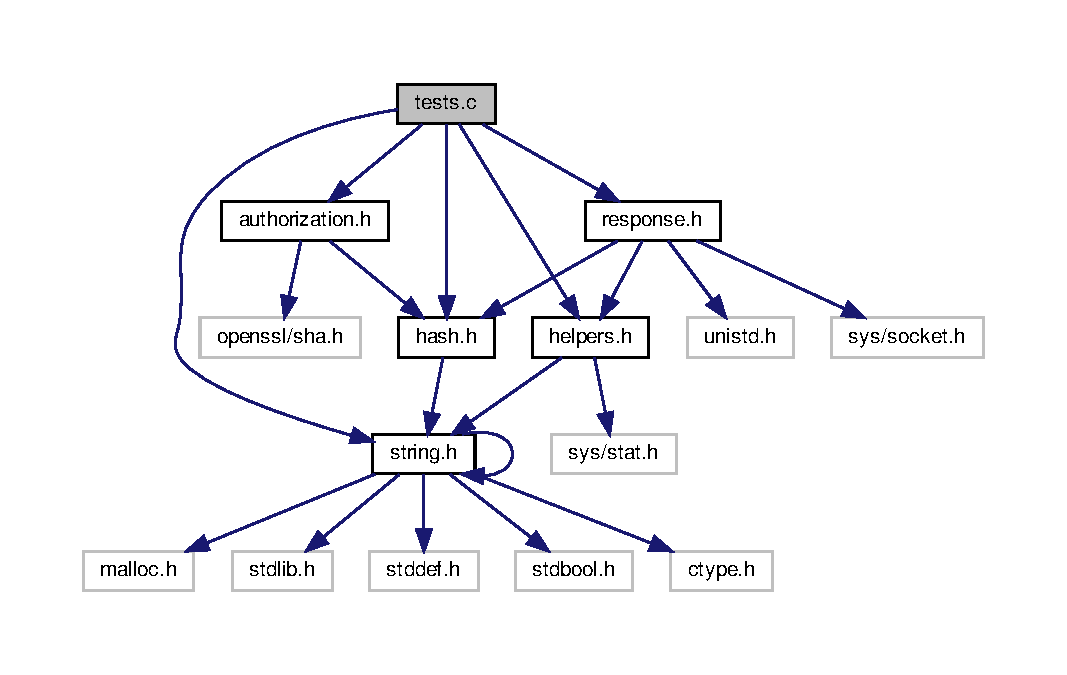
\includegraphics[width=350pt]{tests_8c__incl}
\end{center}
\end{figure}
\subsection*{Functions}
\begin{DoxyCompactItemize}
\item 
void \hyperlink{tests_8c_a581269e90c9435a4cfc31825611ea885}{test\+\_\+hashlist} ()
\item 
void \hyperlink{tests_8c_a4b66981bd9463537eb00d60ea5820b08}{test\+\_\+response\+\_\+build} ()
\item 
void \hyperlink{tests_8c_abc040770b7b1bbb572ba582249354967}{test\+\_\+string\+\_\+split} ()
\item 
void \hyperlink{tests_8c_a7c997dccd2cdd7a55060e20c1616b962}{test\+\_\+get\+\_\+ctype} ()
\item 
void \hyperlink{tests_8c_a346703f5f9907490bb8a4e487ffe7ca2}{test\+\_\+string\+\_\+insert} ()
\item 
void \hyperlink{tests_8c_a917c589685303406fdb43b72267ccc95}{test\+\_\+string\+\_\+split\+\_\+string} ()
\item 
void \hyperlink{tests_8c_a60e79ecc7405286def5e215eb6ca52ed}{test\+\_\+read\+\_\+pw\+\_\+list} ()
\item 
void \hyperlink{tests_8c_a0d076bf6583701c375c0b488d9827d5f}{test\+\_\+str\+\_\+free} ()
\end{DoxyCompactItemize}


\subsection{Function Documentation}
\mbox{\Hypertarget{tests_8c_a7c997dccd2cdd7a55060e20c1616b962}\label{tests_8c_a7c997dccd2cdd7a55060e20c1616b962}} 
\index{tests.\+c@{tests.\+c}!test\+\_\+get\+\_\+ctype@{test\+\_\+get\+\_\+ctype}}
\index{test\+\_\+get\+\_\+ctype@{test\+\_\+get\+\_\+ctype}!tests.\+c@{tests.\+c}}
\subsubsection{\texorpdfstring{test\+\_\+get\+\_\+ctype()}{test\_get\_ctype()}}
{\footnotesize\ttfamily void test\+\_\+get\+\_\+ctype (\begin{DoxyParamCaption}{ }\end{DoxyParamCaption})}

\mbox{\Hypertarget{tests_8c_a581269e90c9435a4cfc31825611ea885}\label{tests_8c_a581269e90c9435a4cfc31825611ea885}} 
\index{tests.\+c@{tests.\+c}!test\+\_\+hashlist@{test\+\_\+hashlist}}
\index{test\+\_\+hashlist@{test\+\_\+hashlist}!tests.\+c@{tests.\+c}}
\subsubsection{\texorpdfstring{test\+\_\+hashlist()}{test\_hashlist()}}
{\footnotesize\ttfamily void test\+\_\+hashlist (\begin{DoxyParamCaption}{ }\end{DoxyParamCaption})}

\mbox{\Hypertarget{tests_8c_a60e79ecc7405286def5e215eb6ca52ed}\label{tests_8c_a60e79ecc7405286def5e215eb6ca52ed}} 
\index{tests.\+c@{tests.\+c}!test\+\_\+read\+\_\+pw\+\_\+list@{test\+\_\+read\+\_\+pw\+\_\+list}}
\index{test\+\_\+read\+\_\+pw\+\_\+list@{test\+\_\+read\+\_\+pw\+\_\+list}!tests.\+c@{tests.\+c}}
\subsubsection{\texorpdfstring{test\+\_\+read\+\_\+pw\+\_\+list()}{test\_read\_pw\_list()}}
{\footnotesize\ttfamily void test\+\_\+read\+\_\+pw\+\_\+list (\begin{DoxyParamCaption}{ }\end{DoxyParamCaption})}

\mbox{\Hypertarget{tests_8c_a4b66981bd9463537eb00d60ea5820b08}\label{tests_8c_a4b66981bd9463537eb00d60ea5820b08}} 
\index{tests.\+c@{tests.\+c}!test\+\_\+response\+\_\+build@{test\+\_\+response\+\_\+build}}
\index{test\+\_\+response\+\_\+build@{test\+\_\+response\+\_\+build}!tests.\+c@{tests.\+c}}
\subsubsection{\texorpdfstring{test\+\_\+response\+\_\+build()}{test\_response\_build()}}
{\footnotesize\ttfamily void test\+\_\+response\+\_\+build (\begin{DoxyParamCaption}{ }\end{DoxyParamCaption})}

\mbox{\Hypertarget{tests_8c_a0d076bf6583701c375c0b488d9827d5f}\label{tests_8c_a0d076bf6583701c375c0b488d9827d5f}} 
\index{tests.\+c@{tests.\+c}!test\+\_\+str\+\_\+free@{test\+\_\+str\+\_\+free}}
\index{test\+\_\+str\+\_\+free@{test\+\_\+str\+\_\+free}!tests.\+c@{tests.\+c}}
\subsubsection{\texorpdfstring{test\+\_\+str\+\_\+free()}{test\_str\_free()}}
{\footnotesize\ttfamily void test\+\_\+str\+\_\+free (\begin{DoxyParamCaption}{ }\end{DoxyParamCaption})}

\mbox{\Hypertarget{tests_8c_a346703f5f9907490bb8a4e487ffe7ca2}\label{tests_8c_a346703f5f9907490bb8a4e487ffe7ca2}} 
\index{tests.\+c@{tests.\+c}!test\+\_\+string\+\_\+insert@{test\+\_\+string\+\_\+insert}}
\index{test\+\_\+string\+\_\+insert@{test\+\_\+string\+\_\+insert}!tests.\+c@{tests.\+c}}
\subsubsection{\texorpdfstring{test\+\_\+string\+\_\+insert()}{test\_string\_insert()}}
{\footnotesize\ttfamily void test\+\_\+string\+\_\+insert (\begin{DoxyParamCaption}{ }\end{DoxyParamCaption})}

\mbox{\Hypertarget{tests_8c_abc040770b7b1bbb572ba582249354967}\label{tests_8c_abc040770b7b1bbb572ba582249354967}} 
\index{tests.\+c@{tests.\+c}!test\+\_\+string\+\_\+split@{test\+\_\+string\+\_\+split}}
\index{test\+\_\+string\+\_\+split@{test\+\_\+string\+\_\+split}!tests.\+c@{tests.\+c}}
\subsubsection{\texorpdfstring{test\+\_\+string\+\_\+split()}{test\_string\_split()}}
{\footnotesize\ttfamily void test\+\_\+string\+\_\+split (\begin{DoxyParamCaption}{ }\end{DoxyParamCaption})}

\mbox{\Hypertarget{tests_8c_a917c589685303406fdb43b72267ccc95}\label{tests_8c_a917c589685303406fdb43b72267ccc95}} 
\index{tests.\+c@{tests.\+c}!test\+\_\+string\+\_\+split\+\_\+string@{test\+\_\+string\+\_\+split\+\_\+string}}
\index{test\+\_\+string\+\_\+split\+\_\+string@{test\+\_\+string\+\_\+split\+\_\+string}!tests.\+c@{tests.\+c}}
\subsubsection{\texorpdfstring{test\+\_\+string\+\_\+split\+\_\+string()}{test\_string\_split\_string()}}
{\footnotesize\ttfamily void test\+\_\+string\+\_\+split\+\_\+string (\begin{DoxyParamCaption}{ }\end{DoxyParamCaption})}


\hypertarget{tests_8h}{}\section{tests.\+h File Reference}
\label{tests_8h}\index{tests.\+h@{tests.\+h}}
{\ttfamily \#include \char`\"{}string.\+h\char`\"{}}\newline
{\ttfamily \#include \char`\"{}helpers.\+h\char`\"{}}\newline
{\ttfamily \#include \char`\"{}hash.\+h\char`\"{}}\newline
{\ttfamily \#include \char`\"{}response.\+h\char`\"{}}\newline
Include dependency graph for tests.\+h\+:
\nopagebreak
\begin{figure}[H]
\begin{center}
\leavevmode
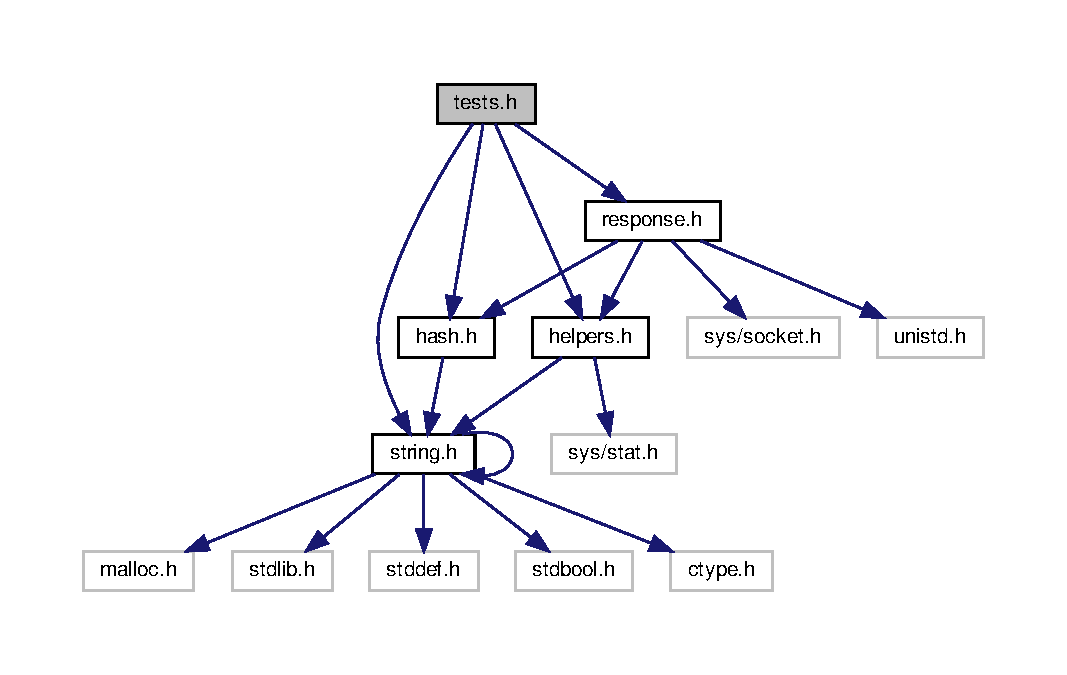
\includegraphics[width=350pt]{tests_8h__incl}
\end{center}
\end{figure}
This graph shows which files directly or indirectly include this file\+:
\nopagebreak
\begin{figure}[H]
\begin{center}
\leavevmode
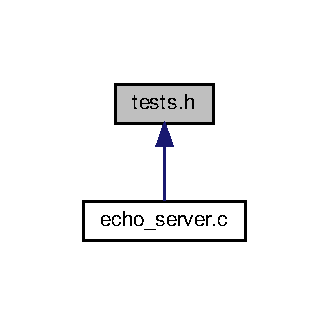
\includegraphics[width=158pt]{tests_8h__dep__incl}
\end{center}
\end{figure}
\subsection*{Functions}
\begin{DoxyCompactItemize}
\item 
void \hyperlink{tests_8h_a581269e90c9435a4cfc31825611ea885}{test\+\_\+hashlist} ()
\item 
void \hyperlink{tests_8h_a4b66981bd9463537eb00d60ea5820b08}{test\+\_\+response\+\_\+build} ()
\item 
void \hyperlink{tests_8h_abc040770b7b1bbb572ba582249354967}{test\+\_\+string\+\_\+split} ()
\item 
void \hyperlink{tests_8h_a7c997dccd2cdd7a55060e20c1616b962}{test\+\_\+get\+\_\+ctype} ()
\item 
void \hyperlink{tests_8h_a346703f5f9907490bb8a4e487ffe7ca2}{test\+\_\+string\+\_\+insert} ()
\item 
void \hyperlink{tests_8h_a917c589685303406fdb43b72267ccc95}{test\+\_\+string\+\_\+split\+\_\+string} ()
\item 
void \hyperlink{tests_8h_a60e79ecc7405286def5e215eb6ca52ed}{test\+\_\+read\+\_\+pw\+\_\+list} ()
\item 
void \hyperlink{tests_8h_a0d076bf6583701c375c0b488d9827d5f}{test\+\_\+str\+\_\+free} ()
\end{DoxyCompactItemize}


\subsection{Function Documentation}
\mbox{\Hypertarget{tests_8h_a7c997dccd2cdd7a55060e20c1616b962}\label{tests_8h_a7c997dccd2cdd7a55060e20c1616b962}} 
\index{tests.\+h@{tests.\+h}!test\+\_\+get\+\_\+ctype@{test\+\_\+get\+\_\+ctype}}
\index{test\+\_\+get\+\_\+ctype@{test\+\_\+get\+\_\+ctype}!tests.\+h@{tests.\+h}}
\subsubsection{\texorpdfstring{test\+\_\+get\+\_\+ctype()}{test\_get\_ctype()}}
{\footnotesize\ttfamily void test\+\_\+get\+\_\+ctype (\begin{DoxyParamCaption}{ }\end{DoxyParamCaption})}

\mbox{\Hypertarget{tests_8h_a581269e90c9435a4cfc31825611ea885}\label{tests_8h_a581269e90c9435a4cfc31825611ea885}} 
\index{tests.\+h@{tests.\+h}!test\+\_\+hashlist@{test\+\_\+hashlist}}
\index{test\+\_\+hashlist@{test\+\_\+hashlist}!tests.\+h@{tests.\+h}}
\subsubsection{\texorpdfstring{test\+\_\+hashlist()}{test\_hashlist()}}
{\footnotesize\ttfamily void test\+\_\+hashlist (\begin{DoxyParamCaption}{ }\end{DoxyParamCaption})}

\mbox{\Hypertarget{tests_8h_a60e79ecc7405286def5e215eb6ca52ed}\label{tests_8h_a60e79ecc7405286def5e215eb6ca52ed}} 
\index{tests.\+h@{tests.\+h}!test\+\_\+read\+\_\+pw\+\_\+list@{test\+\_\+read\+\_\+pw\+\_\+list}}
\index{test\+\_\+read\+\_\+pw\+\_\+list@{test\+\_\+read\+\_\+pw\+\_\+list}!tests.\+h@{tests.\+h}}
\subsubsection{\texorpdfstring{test\+\_\+read\+\_\+pw\+\_\+list()}{test\_read\_pw\_list()}}
{\footnotesize\ttfamily void test\+\_\+read\+\_\+pw\+\_\+list (\begin{DoxyParamCaption}{ }\end{DoxyParamCaption})}

\mbox{\Hypertarget{tests_8h_a4b66981bd9463537eb00d60ea5820b08}\label{tests_8h_a4b66981bd9463537eb00d60ea5820b08}} 
\index{tests.\+h@{tests.\+h}!test\+\_\+response\+\_\+build@{test\+\_\+response\+\_\+build}}
\index{test\+\_\+response\+\_\+build@{test\+\_\+response\+\_\+build}!tests.\+h@{tests.\+h}}
\subsubsection{\texorpdfstring{test\+\_\+response\+\_\+build()}{test\_response\_build()}}
{\footnotesize\ttfamily void test\+\_\+response\+\_\+build (\begin{DoxyParamCaption}{ }\end{DoxyParamCaption})}

\mbox{\Hypertarget{tests_8h_a0d076bf6583701c375c0b488d9827d5f}\label{tests_8h_a0d076bf6583701c375c0b488d9827d5f}} 
\index{tests.\+h@{tests.\+h}!test\+\_\+str\+\_\+free@{test\+\_\+str\+\_\+free}}
\index{test\+\_\+str\+\_\+free@{test\+\_\+str\+\_\+free}!tests.\+h@{tests.\+h}}
\subsubsection{\texorpdfstring{test\+\_\+str\+\_\+free()}{test\_str\_free()}}
{\footnotesize\ttfamily void test\+\_\+str\+\_\+free (\begin{DoxyParamCaption}{ }\end{DoxyParamCaption})}

\mbox{\Hypertarget{tests_8h_a346703f5f9907490bb8a4e487ffe7ca2}\label{tests_8h_a346703f5f9907490bb8a4e487ffe7ca2}} 
\index{tests.\+h@{tests.\+h}!test\+\_\+string\+\_\+insert@{test\+\_\+string\+\_\+insert}}
\index{test\+\_\+string\+\_\+insert@{test\+\_\+string\+\_\+insert}!tests.\+h@{tests.\+h}}
\subsubsection{\texorpdfstring{test\+\_\+string\+\_\+insert()}{test\_string\_insert()}}
{\footnotesize\ttfamily void test\+\_\+string\+\_\+insert (\begin{DoxyParamCaption}{ }\end{DoxyParamCaption})}

\mbox{\Hypertarget{tests_8h_abc040770b7b1bbb572ba582249354967}\label{tests_8h_abc040770b7b1bbb572ba582249354967}} 
\index{tests.\+h@{tests.\+h}!test\+\_\+string\+\_\+split@{test\+\_\+string\+\_\+split}}
\index{test\+\_\+string\+\_\+split@{test\+\_\+string\+\_\+split}!tests.\+h@{tests.\+h}}
\subsubsection{\texorpdfstring{test\+\_\+string\+\_\+split()}{test\_string\_split()}}
{\footnotesize\ttfamily void test\+\_\+string\+\_\+split (\begin{DoxyParamCaption}{ }\end{DoxyParamCaption})}

\mbox{\Hypertarget{tests_8h_a917c589685303406fdb43b72267ccc95}\label{tests_8h_a917c589685303406fdb43b72267ccc95}} 
\index{tests.\+h@{tests.\+h}!test\+\_\+string\+\_\+split\+\_\+string@{test\+\_\+string\+\_\+split\+\_\+string}}
\index{test\+\_\+string\+\_\+split\+\_\+string@{test\+\_\+string\+\_\+split\+\_\+string}!tests.\+h@{tests.\+h}}
\subsubsection{\texorpdfstring{test\+\_\+string\+\_\+split\+\_\+string()}{test\_string\_split\_string()}}
{\footnotesize\ttfamily void test\+\_\+string\+\_\+split\+\_\+string (\begin{DoxyParamCaption}{ }\end{DoxyParamCaption})}


%--- End generated contents ---

% Index
\backmatter
\newpage
\phantomsection
\clearemptydoublepage
\addcontentsline{toc}{chapter}{Index}
\printindex

\end{document}
